% Options for packages loaded elsewhere
\PassOptionsToPackage{unicode}{hyperref}
\PassOptionsToPackage{hyphens}{url}
\documentclass[
]{article}
\usepackage{xcolor}
\usepackage{amsmath,amssymb}
\setcounter{secnumdepth}{5}
\usepackage{iftex}
\ifPDFTeX
  \usepackage[T1]{fontenc}
  \usepackage[utf8]{inputenc}
  \usepackage{textcomp} % provide euro and other symbols
\else % if luatex or xetex
  \usepackage{unicode-math} % this also loads fontspec
  \defaultfontfeatures{Scale=MatchLowercase}
  \defaultfontfeatures[\rmfamily]{Ligatures=TeX,Scale=1}
\fi
% \usepackage{lmodern}
\ifPDFTeX\else
  % xetex/luatex font selection
\fi
% Use upquote if available, for straight quotes in verbatim environments
\IfFileExists{upquote.sty}{\usepackage{upquote}}{}
\IfFileExists{microtype.sty}{% use microtype if available
  \usepackage[]{microtype}
  \UseMicrotypeSet[protrusion]{basicmath} % disable protrusion for tt fonts
}{}
\makeatletter
\@ifundefined{KOMAClassName}{% if non-KOMA class
  \IfFileExists{parskip.sty}{%
    \usepackage{parskip}
  }{% else
    \setlength{\parindent}{0pt}
    \setlength{\parskip}{6pt plus 2pt minus 1pt}}
}{% if KOMA class
  \KOMAoptions{parskip=half}}
\makeatother
\usepackage{color}
\usepackage{fancyvrb}
\newcommand{\VerbBar}{|}
\newcommand{\VERB}{\Verb[commandchars=\\\{\}]}
\DefineVerbatimEnvironment{Highlighting}{Verbatim}{commandchars=\\\{\}}
% Add ',fontsize=\small' for more characters per line
\newenvironment{Shaded}{}{}
\newcommand{\AlertTok}[1]{\textcolor[rgb]{1.00,0.00,0.00}{\textbf{#1}}}
\newcommand{\AnnotationTok}[1]{\textcolor[rgb]{0.38,0.63,0.69}{\textbf{\textit{#1}}}}
\newcommand{\AttributeTok}[1]{\textcolor[rgb]{0.49,0.56,0.16}{#1}}
\newcommand{\BaseNTok}[1]{\textcolor[rgb]{0.25,0.63,0.44}{#1}}
\newcommand{\BuiltInTok}[1]{\textcolor[rgb]{0.00,0.50,0.00}{#1}}
\newcommand{\CharTok}[1]{\textcolor[rgb]{0.25,0.44,0.63}{#1}}
\newcommand{\CommentTok}[1]{\textcolor[rgb]{0.38,0.63,0.69}{\textit{#1}}}
\newcommand{\CommentVarTok}[1]{\textcolor[rgb]{0.38,0.63,0.69}{\textbf{\textit{#1}}}}
\newcommand{\ConstantTok}[1]{\textcolor[rgb]{0.53,0.00,0.00}{#1}}
\newcommand{\ControlFlowTok}[1]{\textcolor[rgb]{0.00,0.44,0.13}{\textbf{#1}}}
\newcommand{\DataTypeTok}[1]{\textcolor[rgb]{0.56,0.13,0.00}{#1}}
\newcommand{\DecValTok}[1]{\textcolor[rgb]{0.25,0.63,0.44}{#1}}
\newcommand{\DocumentationTok}[1]{\textcolor[rgb]{0.73,0.13,0.13}{\textit{#1}}}
\newcommand{\ErrorTok}[1]{\textcolor[rgb]{1.00,0.00,0.00}{\textbf{#1}}}
\newcommand{\ExtensionTok}[1]{#1}
\newcommand{\FloatTok}[1]{\textcolor[rgb]{0.25,0.63,0.44}{#1}}
\newcommand{\FunctionTok}[1]{\textcolor[rgb]{0.02,0.16,0.49}{#1}}
\newcommand{\ImportTok}[1]{\textcolor[rgb]{0.00,0.50,0.00}{\textbf{#1}}}
\newcommand{\InformationTok}[1]{\textcolor[rgb]{0.38,0.63,0.69}{\textbf{\textit{#1}}}}
\newcommand{\KeywordTok}[1]{\textcolor[rgb]{0.00,0.44,0.13}{\textbf{#1}}}
\newcommand{\NormalTok}[1]{#1}
\newcommand{\OperatorTok}[1]{\textcolor[rgb]{0.40,0.40,0.40}{#1}}
\newcommand{\OtherTok}[1]{\textcolor[rgb]{0.00,0.44,0.13}{#1}}
\newcommand{\PreprocessorTok}[1]{\textcolor[rgb]{0.74,0.48,0.00}{#1}}
\newcommand{\RegionMarkerTok}[1]{#1}
\newcommand{\SpecialCharTok}[1]{\textcolor[rgb]{0.25,0.44,0.63}{#1}}
\newcommand{\SpecialStringTok}[1]{\textcolor[rgb]{0.73,0.40,0.53}{#1}}
\newcommand{\StringTok}[1]{\textcolor[rgb]{0.25,0.44,0.63}{#1}}
\newcommand{\VariableTok}[1]{\textcolor[rgb]{0.10,0.09,0.49}{#1}}
\newcommand{\VerbatimStringTok}[1]{\textcolor[rgb]{0.25,0.44,0.63}{#1}}
\newcommand{\WarningTok}[1]{\textcolor[rgb]{0.38,0.63,0.69}{\textbf{\textit{#1}}}}
\usepackage{longtable,booktabs,array}
\newcounter{none} % for unnumbered tables
\usepackage{calc} % for calculating minipage widths
% Correct order of tables after \paragraph or \subparagraph
\usepackage{etoolbox}
\makeatletter
\patchcmd\longtable{\par}{\if@noskipsec\mbox{}\fi\par}{}{}
\makeatother
% Allow footnotes in longtable head/foot
\IfFileExists{footnotehyper.sty}{\usepackage{footnotehyper}}{\usepackage{footnote}}
\makesavenoteenv{longtable}
\usepackage{graphicx}
\makeatletter
\newsavebox\pandoc@box
\newcommand*\pandocbounded[1]{% scales image to fit in text height/width
  \sbox\pandoc@box{#1}%
  \Gscale@div\@tempa{\textheight}{\dimexpr\ht\pandoc@box+\dp\pandoc@box\relax}%
  \Gscale@div\@tempb{\linewidth}{\wd\pandoc@box}%
  \ifdim\@tempb\p@<\@tempa\p@\let\@tempa\@tempb\fi% select the smaller of both
  \ifdim\@tempa\p@<\p@\scalebox{\@tempa}{\usebox\pandoc@box}%
  \else\usebox{\pandoc@box}%
  \fi%
}
% Set default figure placement to htbp
\def\fps@figure{htbp}
\makeatother
\setlength{\emergencystretch}{3em} % prevent overfull lines
\providecommand{\tightlist}{%
  \setlength{\itemsep}{0pt}\setlength{\parskip}{0pt}}
\usepackage[]{natbib}
\bibliographystyle{plainnat}
\usepackage{bookmark}
\IfFileExists{xurl.sty}{\usepackage{xurl}}{} % add URL line breaks if available
\urlstyle{same}
\hypersetup{
  pdftitle={Notation and Terminology},
  hidelinks,
  pdfcreator={LaTeX via pandoc}}

\title{Notation and Terminology}
\author{}
\date{}

\title{A Cognitive Case for Diagrams\\\normalsize Category-Theoretic Approaches to Linguistic Case Systems, Cognitive Modeling, and AI Communication}
\author{Daniel Ari Friedman\\\footnotesize{Active Inference Institute}\\\footnotesize{\texttt{daniel@activeinference.institute}}\\\footnotesize{\href{https://orcid.org/0000-0001-6232-9096}{ORCID: 0000-0001-6232-9096}}}
\date{\today}

% Core mathematics
\usepackage{amsmath}
\usepackage{amssymb}
\usepackage{amsfonts}
\usepackage{amsthm}

% Equation numbering by section
\numberwithin{equation}{section}

% Category theory diagrams
\usepackage{tikz-cd}

% Document layout — tighter margins for review drafts
\usepackage[margin=1in]{geometry}
\usepackage{float}
\usepackage{graphicx}

% Tables
\usepackage{booktabs}
\usepackage{longtable}
\usepackage{array}
\usepackage{caption}

% Typography and formatting
\usepackage{microtype}
\usepackage{xcolor}

% Start new main sections on a new page
\usepackage{titlesec}
\newcommand{\sectionbreak}{\clearpage}

% Cross-references and citations — all links red, auto-refs
% NOTE: hyperref is loaded by Pandoc; use \hypersetup to configure it
\hypersetup{colorlinks=true,linkcolor=red,citecolor=red,urlcolor=red}
\usepackage[capitalise,noabbrev]{cleveref}
\usepackage{natbib}

\makeatletter
\AtBeginDocument{\immediate\write\@auxout{\string\bibdata{references}}}
\makeatother
\begin{document}
\maketitle
\thispagestyle{empty}
\tableofcontents
\newpage

\section{Abstract}\label{abstract}

This review unifies four converging research programmes---case systems
in theoretical linguistics, categorial grammar and its
string-diagrammatic semantics, enriched and topos-theoretic category
theory, and active inference as a process theory of cognition---into a
single coherent framework centred on the \emph{cognitive case diagram}.
The formal core treats case systems as categories (objects = case roles,
morphisms = grammatical relations), cross-linguistic alignment types as
functors between case categories, and sentences as compact-closed string
diagrams in the DisCoCat (Distributional Compositional Categorical)
framework. By demonstrating that DisCoCat constitutes the algebraic
formalization of the distributional programme that modern large language
models implement empirically---from static word embeddings through
contextual transformers---we bridge the two traditions of meaning
(formal and distributional) within a unified categorical architecture.
These diagrams serve simultaneously as mathematical proofs, cognitive
representations, and the structural core of generative models under
active inference: understanding a sentence reduces to constructing the
case diagram that minimizes variational free energy. We extend this
framework through Distributional Active Inference, which models full
distributions over case diagrams rather than point estimates, connecting
distributional semantics to distributional reinforcement learning via
enriched-categorical push-forward measures. Graded proto-role structure
is captured via \([0,1]\)-enriched categories with categorical magnitude
as a complexity measure, and inter-theoretic translation is formalized
through Morita-equivalent classifying toposes. Implementation within the
CEREBRUM (Case-Enabled Reasoning Engine with Bayesian Representations
for Unified Models) architecture demonstrates practical viability. The
analysis suggests that the mathematics of case alignment is not merely
an abstraction of human grammar, but the formal geometry of relational
meaning itself---the architecture through which cognitive systems
organize experience into who-does-what-to-whom.

\newpage

\section{Introduction}\label{sec:introduction}

\subsection{The Problem of Case Assignment in Cognitive
Scenarios}\label{the-problem-of-case-assignment-in-cognitive-scenarios}

Every natural language encodes relational structure---\emph{who does
what to whom, with what, where, and why}---through some form of case
system. In morphologically rich languages such as Finnish, Latin, or
Sanskrit, this encoding is overt: distinct suffixes mark the agent,
patient, instrument, and location of an event. In languages like
Mandarin or English, the same relational skeleton is expressed through
word order, adpositions, or construction-level patterns. Despite the
surface variation, the underlying computational problem is universal: a
cognitive agent must assign \emph{structured roles} to the participants
of every scenario it encounters, predicts, or plans.

This universality suggests that case is not merely a morphosyntactic
accident but a reflection of deep cognitive architecture---a hypothesis
that traces back to Fillmore's \citeyearpar{fillmore1968case} ``Case for
Case,'' which posited a universal inventory of \emph{deep cases} (Agent,
Patient, Instrument, Locative, etc.) underlying all surface-level
grammatical relations. Fillmore's intuition was prescient: subsequent
typological work by Polinsky and Preminger
\citeyearpar{polinsky2015case}, Blake
\citeyearpar{blake2001grammatical}, and Haspelmath
\citeyearpar{haspelmath2009universality} has confirmed that while
languages vary enormously in how they package case, the space of
variation is itself structured---it can be organized into a small number
of \emph{alignment types} (nominative--accusative, ergative--absolutive,
active--stative, tripartite, fluid-S) related by systematic
transformations.

This review highlights how \textbf{category theory} provides the natural
mathematical language for formalizing this structure, and how
\textbf{commutative diagrams} function not merely as convenient notation
for category-theoretic reasoning but as \emph{cognitively privileged
representations} that provide inferential advantages unavailable to
purely sentential encodings.

\subsection{Why Diagrams? The Cognitive Science of Diagrammatic
Reasoning}\label{why-diagrams-the-cognitive-science-of-diagrammatic-reasoning}

The cognitive science of diagrammatic reasoning provides a strong
empirical foundation for this claim. Larkin and Simon
\citeyearpar{larkin1987diagram} demonstrated that diagrams can be
computationally superior to sentential representations: their
two-dimensional spatial structure enables efficient search, grouping,
and direct perceptual recognition of relationships that would require
explicit inference steps in a text-based format. Shimojima
\citeyearpar{shimojima1996reasoning} refined this insight with the
concept of \emph{free ride inferences}---conclusions that emerge
automatically from the spatial properties of a diagram without any
syntactic manipulation.

In the context of case theory, commutative diagrams offer precisely
these advantages. A commutative triangle expressing that morphism
\(g \circ f\) equals morphism \(h\) simultaneously encodes:

\begin{enumerate}
\def\labelenumi{\arabic{enumi}.}
\tightlist
\item
  The compositional structure of the relation (two steps factor through
  an intermediate case role)
\item
  The \emph{commutativity constraint} (the direct and indirect routes
  yield the same result)
\item
  The full relational context (all three objects and all paths between
  them are visible at once)
\end{enumerate}

This is exactly the kind of information that is difficult to extract
from a linear notation but jumps out from a diagram.
\autoref{fig:case-minimal} illustrates this with a minimal three-case
category where the composition of ``acts\_on'' and ``applied\_to''
factors through the instrument role. As Giardino
\citeyearpar{giardino2017diagrammatic} emphasizes, mathematical diagrams
engage a hybrid mode of reasoning that combines perceptual pattern
recognition with background theoretical knowledge---a mode that aligns
naturally with the predictive processing architecture of active
inference \citep{friston2017active}.

\begin{figure}
\centering
\pandocbounded{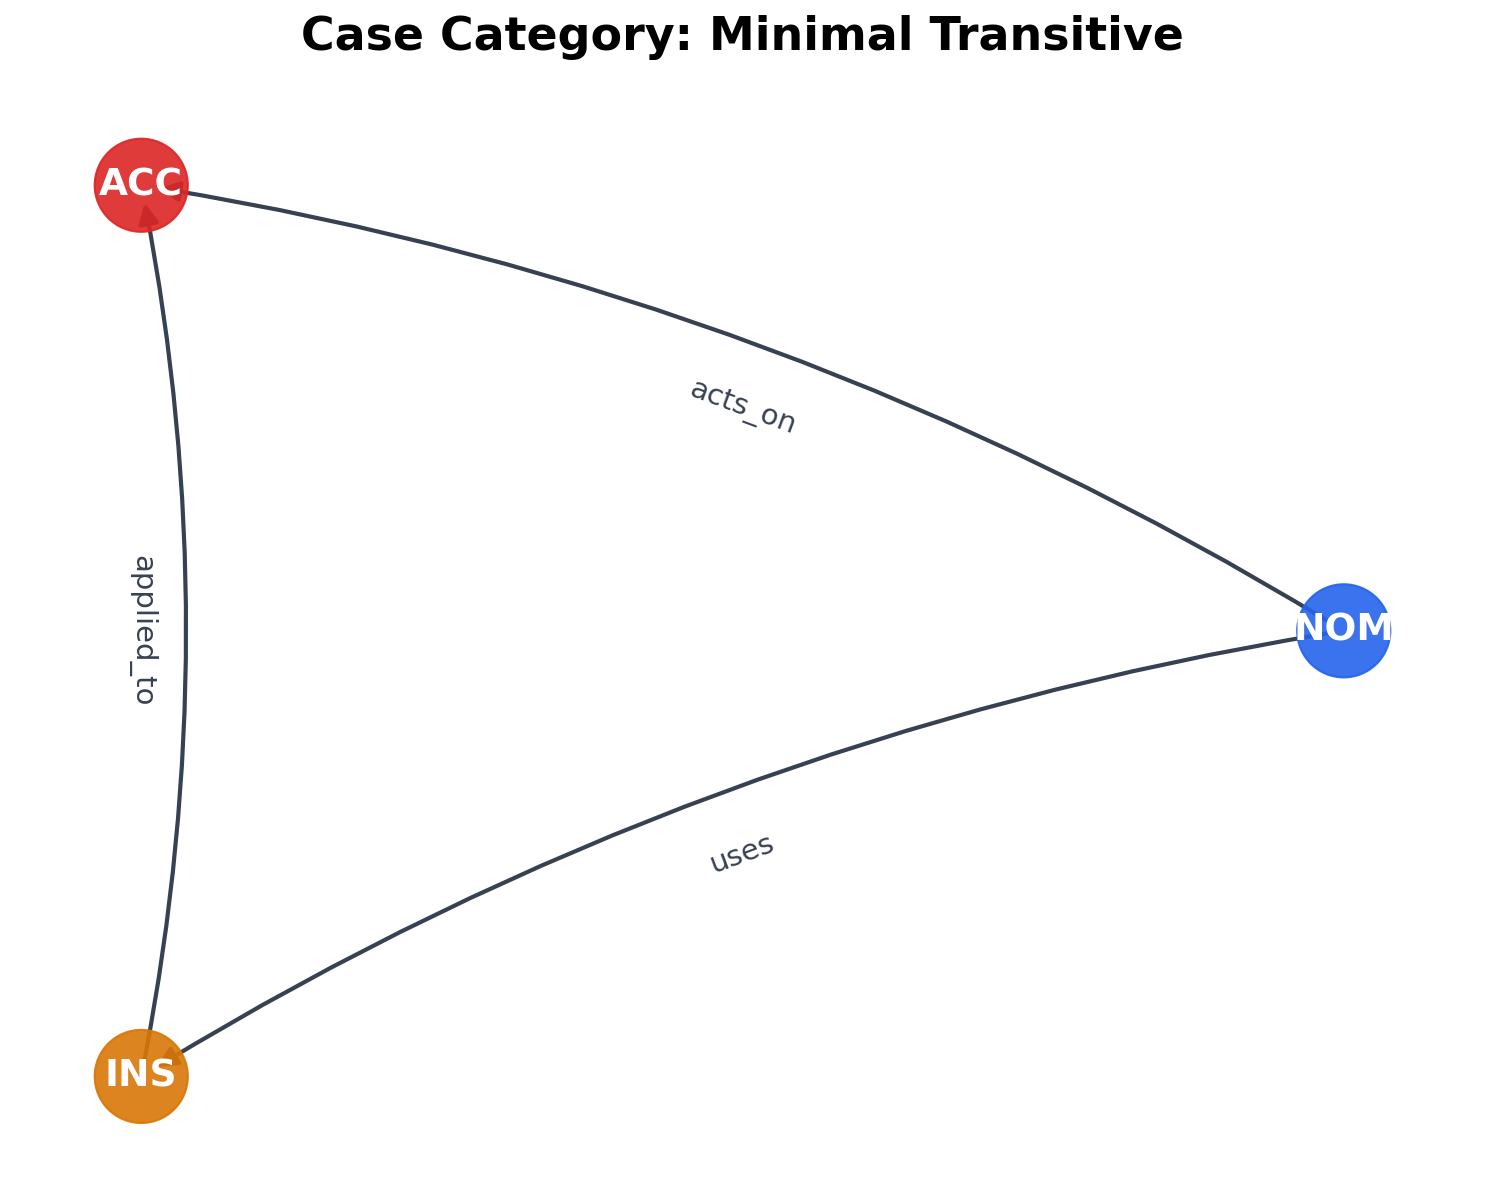
\includegraphics[keepaspectratio,alt={A minimal case category with three objects---Agent (NOM), Patient (ACC), and Instrument (INS)---and three morphisms: `acts\_on' (NOM to ACC), `applied\_to' (INS to ACC), and the composite `acts\_via' (NOM to INS to ACC). The commutative triangle makes the factorization through the instrument role visually immediate, illustrating how two-dimensional layout provides a free-ride inference that linear notation obscures.}]{../figures/case_category_minimal.png}}
\caption{A minimal case category with three objects---Agent (NOM),
Patient (ACC), and Instrument (INS)---and three morphisms: `acts\_on'
(NOM to ACC), `applied\_to' (INS to ACC), and the composite `acts\_via'
(NOM to INS to ACC). The commutative triangle makes the factorization
through the instrument role visually immediate, illustrating how
two-dimensional layout provides a free-ride inference that linear
notation obscures.}\label{fig:case-minimal}
\end{figure}

\subsection{Five Converging Research
Pillars}\label{five-converging-research-pillars}

The present synthesis draws on five research traditions, each
contributing an essential formal ingredient:

\subsubsection{Pillar 1: Case Systems, Alignment Typology, and
Grammatical
Relations}\label{pillar-1-case-systems-alignment-typology-and-grammatical-relations}

The empirical foundation comes from linguistic typology. We formalize
the case inventory and alignment systems catalogued by Polinsky and
Preminger \citeyearpar{polinsky2015case}, Claassen
\citeyearpar{claassen2025alignment}, and Wu \citeyearpar{wu2024amis} as
categories with case roles as objects and grammatical relations as
morphisms. Dowty's \citeyearpar{dowty1991thematic} proto-role
theory---which decomposes thematic roles into clusters of entailments
rather than discrete atoms---motivates our use of enriched (weighted)
morphisms.

\subsubsection{Pillar 2: Categorial and Type-Theoretic
Grammar}\label{pillar-2-categorial-and-type-theoretic-grammar}

Lambek's \citeyearpar{lambek1958mathematics} syntactic calculus
reformulates grammatical combination as algebraic cancellation in a
pregroup, yielding derivations that can be visualized as Joyal and
Street's \citeyearpar{joyalstreet1991geometry} string diagrams. Song
\citeyearpar{song2022act} extends this with monadic semantics for root
syntax, showing that category-theoretic structure reaches down to the
sublexical level.

\subsubsection{Pillar 3: Categorical Compositional Distributional
Semantics
(DisCoCat)}\label{pillar-3-categorical-compositional-distributional-semantics-discocat}

Coecke, Sadrzadeh, and Clark's \citeyearpar{coecke2010mathematical}
DisCoCat framework composes distributional word meanings according to
syntactic structure using monoidal categories and string diagrams. This
framework bridges the two great traditions of linguistic
meaning---formal (truth-conditional, compositional) and distributional
(context-dependent, statistical)---by using the algebra of compact
closed categories to compose vector representations according to
type-logical derivations. The resulting categorical semantics provides
the \emph{algebraic formalization} of the distributional programme that
modern large language models (from Word2Vec \citep{mikolov2013efficient}
through transformer architectures
\citep{vaswani2017attention, devlin2019bert}) implement empirically,
making it possible to analyse both symbolic and neural approaches to
language within a single mathematical framework. Recent extensions
include DisCoCirc \citep{defelice2020discourse, defelice2022discocirc}
for discourse-level coherence and the lambeq library
\citep{lorenz2023lambeq} for quantum NLP, which implements the full
categorical pipeline on quantum hardware.

\subsubsection{Pillar 4: Enriched Category Theory and Distributional
Measures}\label{pillar-4-enriched-category-theory-and-distributional-measures}

Bradley et al.'s \citeyearpar{fritz2021enriched} enrichment over
\([0,1]\) equips hom-sets with distributional proximity measures.
Bradley's
\citetext{\citeyear{bradley2020entropy}; \citeyear{bradley2024ipam}}
work on topological operads and categorical magnitude provides
information-theoretic invariants that quantify the ``effective size'' of
a linguistic category---a measure that captures how much distributional
information the category encodes.

\subsubsection{Pillar 5: Topos-Theoretic Bridges and Inter-Theoretic
Transfer}\label{pillar-5-topos-theoretic-bridges-and-inter-theoretic-transfer}

Caramello's
\citetext{\citeyear{caramello2016bridges}; \citeyear{caramello2021five}; \citeyear{caramello2023syntactic}}
bridge technique uses classifying toposes as transfer points between
mathematical theories, enabling results proved in one formalization of
case to port automatically to another. Phillips
\citeyearpar{phillips2024lot} strengthens this by showing that the
Language of Thought admits universal constructions in a topos, grounding
the systematicity of case assignment in the deepest structures of
categorical logic.

\subsection{Unifying Integration: Active Inference and the CEREBRUM
Architecture}\label{unifying-integration-active-inference-and-the-cerebrum-architecture}

The unifying framework is \textbf{active inference}
\citep{friston2017active}, which casts cognition as approximate Bayesian
inference under a generative model. Case-marked commutative diagrams
serve as the structural core of such generative models: each diagram
specifies a pattern of expected relational dependencies, and the agent's
task in understanding (or producing) a sentence is to minimize surprise
relative to this diagrammatic prior. The \textbf{CEREBRUM} architecture
\citep{friedman2024cerebrum}---Case-Enabled Reasoning Engine with
Bayesian Representations for Unified Modeling---provides a computational
instantiation of this framework, with case roles as functional
specializations of model components in an active inference cycle.

This integration is not merely metaphorical. The situation semantics of
Barwise and Perry \citeyearpar{barwise1983situations} already
conceptualized meaning as structured \emph{situations} with typed
constituents---an ontology that maps naturally onto the objects and
morphisms of our case categories. Active inference adds dynamics: the
agent actively samples evidence to confirm or update its case
assignments, using diagrammatic structure to guide exploration.

\subsection{Paper Outline and Chapter
Overview}\label{paper-outline-and-chapter-overview}

The remainder of the paper is organized as follows.
\autoref{sec:case-systems} reviews case systems and alignment typology.
\autoref{sec:categorial-grammar} develops the categorial grammar
foundations. \autoref{sec:categorical-semantics} presents DisCoCat and
its extensions. \autoref{sec:enriched-categories} introduces enriched
categories. \autoref{sec:topos-theory} develops the topos-theoretic
bridges. \autoref{sec:cognitive-integration} integrates everything
within active inference and CEREBRUM. \autoref{sec:ai-implications}
develops implications for synthetic and artificial intelligence.
\autoref{sec:conclusion} concludes with future directions.

\newpage

\section{Case Systems, Grammatical Relations, and Alignment
Typology}\label{sec:case-systems}

\subsection{Historical Foundations: From Pāṇini to Jakobson, Fillmore,
and
Mel'čuk}\label{historical-foundations-from-pux101ux1e47ini-to-jakobson-fillmore-and-melux10duk}

The formal study of grammatical case begins with the Sanskrit grammarian
Pāṇini (c.~4th-5th century BCE), whose \emph{Aṣṭādhyāyī} formalized the
\emph{Kāraka} theory --- a semantic system of deep roles (e.g., agent,
patient) linking nouns to verbs in Sanskrit grammar. Etymologically
meaning ``that which brings about'' an action, the Kāraka system
expresses world knowledge through rigorous mappings from deep semantic
relations to phonological representations via case endings. As later
structuralists noted, ``Semantics and phonetics have been the basis of
all linguistic analysis in the Sanskritic tradition\ldots{} providing
steps for semantic interpretation through carefully crafted
morpho-syntactic procedures''
\citetext{\citeyear{jha2021sanskrit}; \citeyear{kak1987paninian}}.

This profound insight---that a finite set of relational roles underlies
the infinite variety of sentences---was resurrected in modern
linguistics by Charles Fillmore's seminal ``The Case for Case'' (1968),
which explicitly acknowledged its Pāṇinian inheritance while proposing
\emph{deep cases} (Agentive, Objective, Dative) as universal semantic
primitives \citeyearpar{fillmore1968case}. In parallel, structuralist
formalisms pioneered by Roman Jakobson in \emph{Morphologic Inquiry into
Slavic Declension} (1958) and Louis Hjelmslev in \emph{La catégorie des
cas} (1935) treated case not merely as semantic markers, but as formal
systems of paradigmatic and syntagmatic oppositions --- treating cases
as bundles of structural features rather than isolated labels
\citetext{\citeyear{jakobson1958morphologic}; \citeyear{hjelmslev1935categorie}}.

Fillmore's deep cases were precursors to modern \emph{thematic role}
theory. Dowty \citeyearpar{dowty1991thematic} refined the approach by
decomposing thematic roles into clusters of sentential entailments,
yielding two \emph{proto-roles}: the Proto-Agent (characterized by
volitional involvement, sentience, causation, movement) and the
Proto-Patient (characterized by undergoing change of state, incremental
theme, causal affectedness, stationary relative to another participant).
This decomposition is significant for our categorical formalization
because it replaces a discrete role inventory with a \emph{graded}
structure---morphisms in our case category can carry weights reflecting
the degree to which a noun phrase satisfies proto-role entailments.

Between Pāṇini and Fillmore, the structuralist and functionalist
traditions of the early 20th century---particularly those rooted in
Russian and Slavic linguistics---laid essential groundwork. Roman
Jakobson's 1936 formalization of the Russian six-case system
(nominative, genitive, dative, accusative, instrumental, prepositional)
employed binary distinctive features (e.g., {[}±directional{]},
{[}±peripheral{]}), treating case oppositions analogously to
phonological oppositions and revealing that morphological paradigms
possess an internal algebraic structure. The Prague Linguistic Circle,
led by Nikolai Trubetzkoy and Sergej Karcevskij alongside Jakobson,
extended this functionalist analysis to Czech and other Slavic
languages, emphasizing \emph{markedness} hierarchies and the
communicative load of case distinctions---insights that anticipate the
weighted morphisms of our categorical framework. Louis Hjelmslev's
glossematics (1930s--1940s), though Danish in origin, resonated deeply
within Slavic formalism by positing case as a purely relational category
within a sign/content dichotomy, prefiguring Fillmore's abstractions
from surface morphology. Igor Mel'čuk's Meaning-Text Theory
(1970s--present) models Russian case assignment through deep syntactic
actants mapped to surface cases via dependency trees, providing a
computationally explicit formalization that bridges the gap between
Fillmore's semantic roles and contemporary distributional semantics.

\subsection{The Cross-Linguistic Typological
Landscape}\label{the-cross-linguistic-typological-landscape}

Contemporary typological work reveals that the world's languages realize
case systems according to a small number of \emph{alignment
types}---systematic patterns governing how the core arguments of
transitive and intransitive clauses are grouped
\citep{polinsky2015case, blake2001grammatical, haspelmath2009universality}.

\subsubsection{Core Argument Roles}\label{core-argument-roles}

The cross-linguistic comparison rests on three primitives:

{\def\LTcaptype{none} % do not increment counter
\begin{longtable}[]{@{}
  >{\centering\arraybackslash}p{(\linewidth - 4\tabcolsep) * \real{0.3571}}
  >{\raggedright\arraybackslash}p{(\linewidth - 4\tabcolsep) * \real{0.3571}}
  >{\raggedright\arraybackslash}p{(\linewidth - 4\tabcolsep) * \real{0.2857}}@{}}
\toprule\noalign{}
\begin{minipage}[b]{\linewidth}\centering
Symbol
\end{minipage} & \begin{minipage}[b]{\linewidth}\raggedright
Role
\end{minipage} & \begin{minipage}[b]{\linewidth}\raggedright
Definition
\end{minipage} \\
\midrule\noalign{}
\endhead
\bottomrule\noalign{}
\endlastfoot
\textbf{S} & Sole argument of intransitive & ``The child
\textbf{sleeps}'' \\
\textbf{A} & Agent-like argument of transitive & ``\textbf{The child}
broke the vase'' \\
\textbf{P} & Patient-like argument of transitive & ``The child broke
\textbf{the vase}'' \\
\end{longtable}
}

\subsubsection{Alignment Systems}\label{alignment-systems}

The key insight from typological research is that languages differ in
how they \emph{group} these three roles for purposes of case marking,
agreement, and other grammatical processes:

{\def\LTcaptype{none} % do not increment counter
\begin{longtable}[]{@{}
  >{\raggedright\arraybackslash}p{(\linewidth - 4\tabcolsep) * \real{0.3333}}
  >{\raggedright\arraybackslash}p{(\linewidth - 4\tabcolsep) * \real{0.3333}}
  >{\raggedright\arraybackslash}p{(\linewidth - 4\tabcolsep) * \real{0.3333}}@{}}
\toprule\noalign{}
\begin{minipage}[b]{\linewidth}\raggedright
Alignment
\end{minipage} & \begin{minipage}[b]{\linewidth}\raggedright
Grouping
\end{minipage} & \begin{minipage}[b]{\linewidth}\raggedright
Exemplar Languages
\end{minipage} \\
\midrule\noalign{}
\endhead
\bottomrule\noalign{}
\endlastfoot
\textbf{Nominative--Accusative} & S = A \(\neq\) P & English, Latin,
Finnish, Russian \\
\textbf{Ergative--Absolutive} & S = P \(\neq\) A & Basque, Dyirbal,
Georgian (partly) \\
\textbf{Active--Stative} & S splits by agentivity & Lakhota, Guaraní,
Eastern Pomo \\
\textbf{Tripartite} & S \(\neq\) A \(\neq\) P & Nez Perce, some
Australian languages \\
\textbf{Fluid-S} & S marking varies by context & Bats (NE Caucasian),
Acehnese \\
\end{longtable}
}

Claassen \citeyearpar{claassen2025alignment} provides a comprehensive
survey of the explanatory frameworks proposed for alignment diversity,
arguing that no single factor (processing efficiency, disambiguation,
discourse pragmatics) suffices---a conclusion that motivates our
multi-dimensional categorical formalization. Wu \citeyearpar{wu2024amis}
offers a detailed case study of Amis (Austronesian), demonstrating how
verb classification, case marking, and grammatical relations interact in
a language that defies simple alignment classification.

\subsubsection{Extended Case Inventories and the CEREBRUM
Framework}\label{extended-case-inventories-and-the-cerebrum-framework}

Beyond the three core arguments, languages distinguish a rich inventory
of oblique cases. Our formalization follows the CEREBRUM framework
\citep{friedman2024cerebrum} in adopting eight fundamental cases:

{\def\LTcaptype{none} % do not increment counter
\begin{longtable}[]{@{}
  >{\raggedright\arraybackslash}p{(\linewidth - 6\tabcolsep) * \real{0.2353}}
  >{\centering\arraybackslash}p{(\linewidth - 6\tabcolsep) * \real{0.2941}}
  >{\raggedright\arraybackslash}p{(\linewidth - 6\tabcolsep) * \real{0.2353}}
  >{\raggedright\arraybackslash}p{(\linewidth - 6\tabcolsep) * \real{0.2353}}@{}}
\toprule\noalign{}
\begin{minipage}[b]{\linewidth}\raggedright
Case
\end{minipage} & \begin{minipage}[b]{\linewidth}\centering
Abbreviation
\end{minipage} & \begin{minipage}[b]{\linewidth}\raggedright
Semantic Core
\end{minipage} & \begin{minipage}[b]{\linewidth}\raggedright
Syntactic Prototype
\end{minipage} \\
\midrule\noalign{}
\endhead
\bottomrule\noalign{}
\endlastfoot
Nominative & NOM & Agent / experiencer & Intransitive subject,
transitive agent \\
Accusative & ACC & Patient / theme & Direct object, incremental theme \\
Genitive & GEN & Possessor / source & Possessive modifier, partitive \\
Dative & DAT & Recipient / goal & Indirect object, beneficiary \\
Instrumental & INS & Instrument / means & Adverbial of means \\
Locative & LOC & Location / context & Spatial/temporal ground \\
Ablative & ABL & Origin / cause & Source of motion, causal adjunct \\
Vocative & VOC & Addressee & Direct address \\
\end{longtable}
}

\subsection{Categorical Formalization of Case
Systems}\label{categorical-formalization-of-case-systems}

\subsubsection{Case Categories as Directed
Graphs}\label{case-categories-as-directed-graphs}

We define a \textbf{case category} \(\mathcal{C}\) as a small category
where:

\begin{itemize}
\tightlist
\item
  \textbf{Objects} are case roles (NOM, ACC, GEN, DAT, INS, LOC, ABL,
  VOC)
\item
  \textbf{Morphisms} are grammatical relations between roles (e.g.,
  ``transitive action'': NOM → ACC)
\item
  \textbf{Identity morphisms} represent the reflexive relation of each
  case role to itself
\item
  \textbf{Composition} models the transitivity of grammatical
  dependencies
\end{itemize}

This formalization is implemented in our \texttt{CaseCategory} class,
which uses a directed graph (via NetworkX) as the underlying
representation. Each object carries its role enum and optional
morphosyntactic features; each morphism carries a relation label and an
enriched weight \(w \in [0,1]\). \autoref{fig:case-standard} shows the
full eight-case standard category.

\begin{figure}
\centering
\pandocbounded{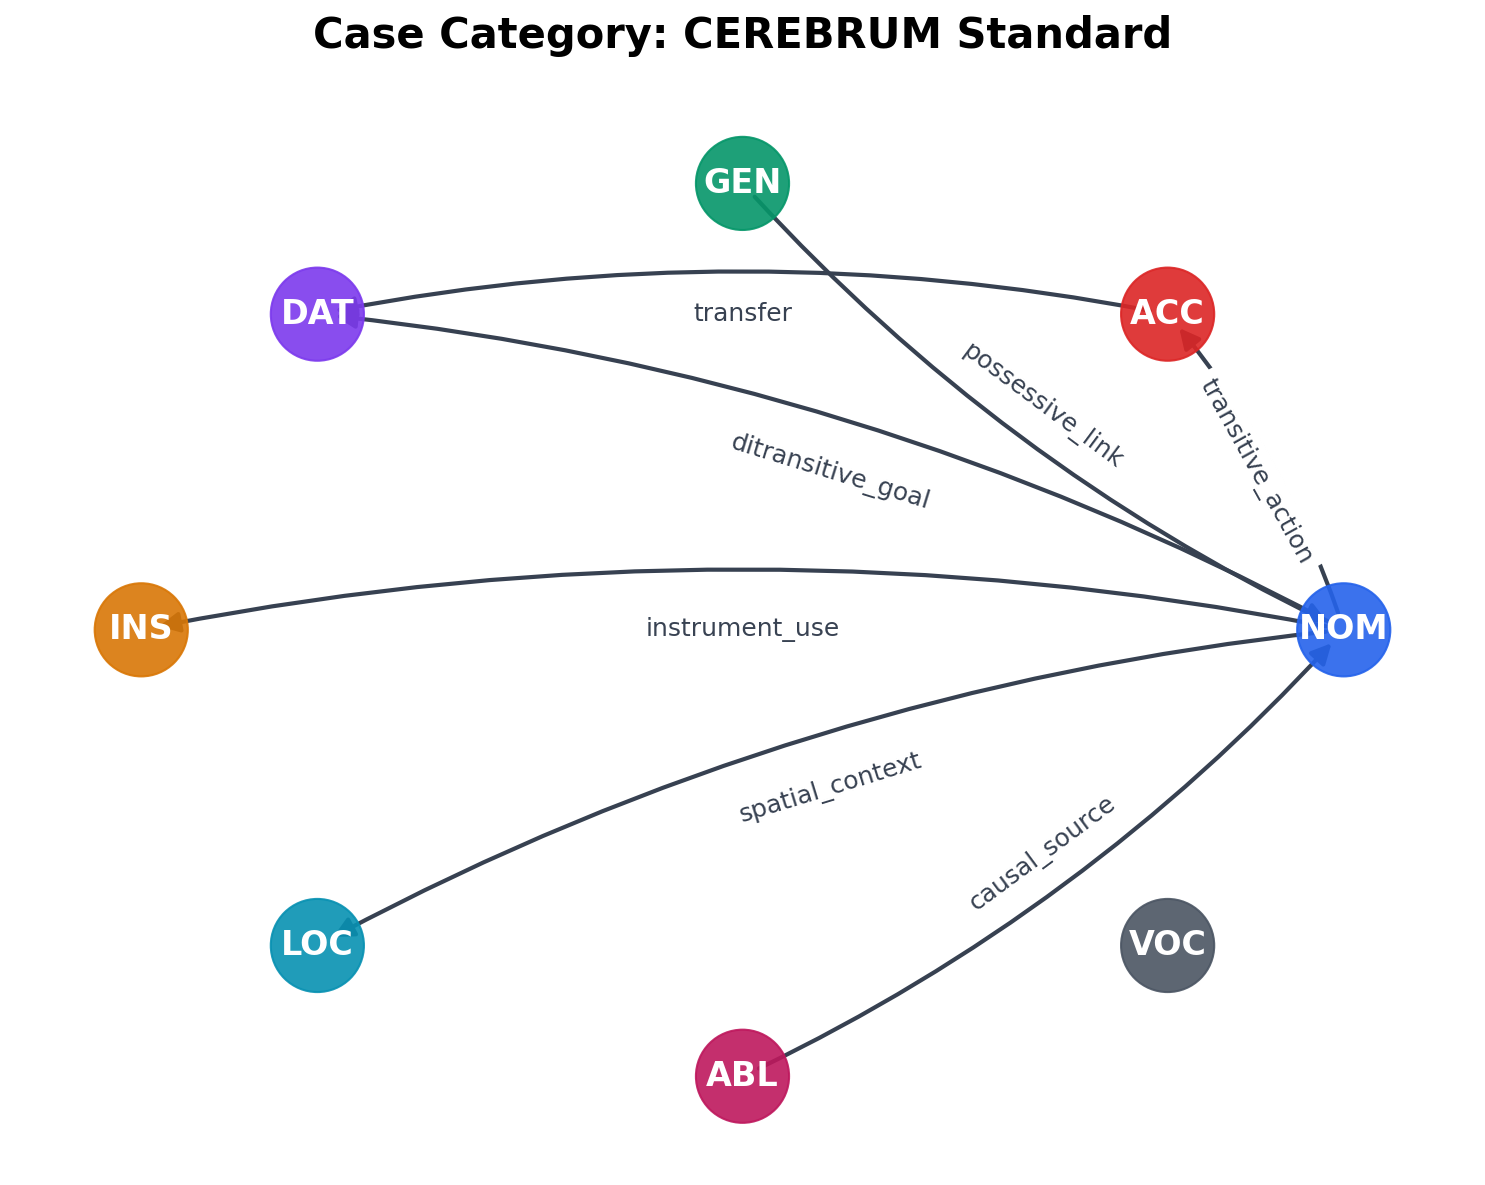
\includegraphics[keepaspectratio,alt={The standard linguistic case category with eight case roles (NOM, ACC, GEN, DAT, INS, LOC, ABL, VOC) and directed morphisms representing grammatical relations between them. Edge labels encode relation types (e.g., transitive action, possession, spatial grounding), and edge weights in the interval zero to one reflect proto-role satisfaction. Generated from the CaseCategory class.}]{../figures/case_category_standard.png}}
\caption{The standard linguistic case category with eight case roles
(NOM, ACC, GEN, DAT, INS, LOC, ABL, VOC) and directed morphisms
representing grammatical relations between them. Edge labels encode
relation types (e.g., transitive action, possession, spatial grounding),
and edge weights in the interval zero to one reflect proto-role
satisfaction. Generated from the CaseCategory
class.}\label{fig:case-standard}
\end{figure}

\subsubsection{Alignment Functors Between Case
Categories}\label{alignment-functors-between-case-categories}

An \textbf{alignment functor} \(F: \mathcal{U} \to \mathcal{L}\) maps a
universal (maximal) case category \(\mathcal{U}\) to a language-specific
category \(\mathcal{L}\) by collapsing objects that a particular
language treats as equivalent. For example, in an accusative language,
the functor merges S and A into a single NOM role while keeping P as a
distinct ACC role: \(F(\text{S}) = F(\text{A}) = \text{NOM}\),
\(F(\text{P}) = \text{ACC}\).

This functor is:

\begin{itemize}
\tightlist
\item
  \textbf{Surjective on objects}: every case in the target language is
  the image of some universal role
\item
  \textbf{Structure-preserving}: grammatical relations in
  \(\mathcal{U}\) map to grammatical relations in \(\mathcal{L}\)
\item
  \textbf{Non-identity when alignment differs}: the kernel of \(F\) (the
  set of objects mapped to the same target) characterizes the alignment
  type
\end{itemize}

The alignment functor provides a formal account of neutralization: two
semantically distinct roles (S vs.~A) receive the same morphological
treatment because the functor maps them to the same object.
\autoref{fig:alignment} shows three alignment systems rendered from our
\texttt{CaseCategory} implementation.

\begin{figure}
\centering
\pandocbounded{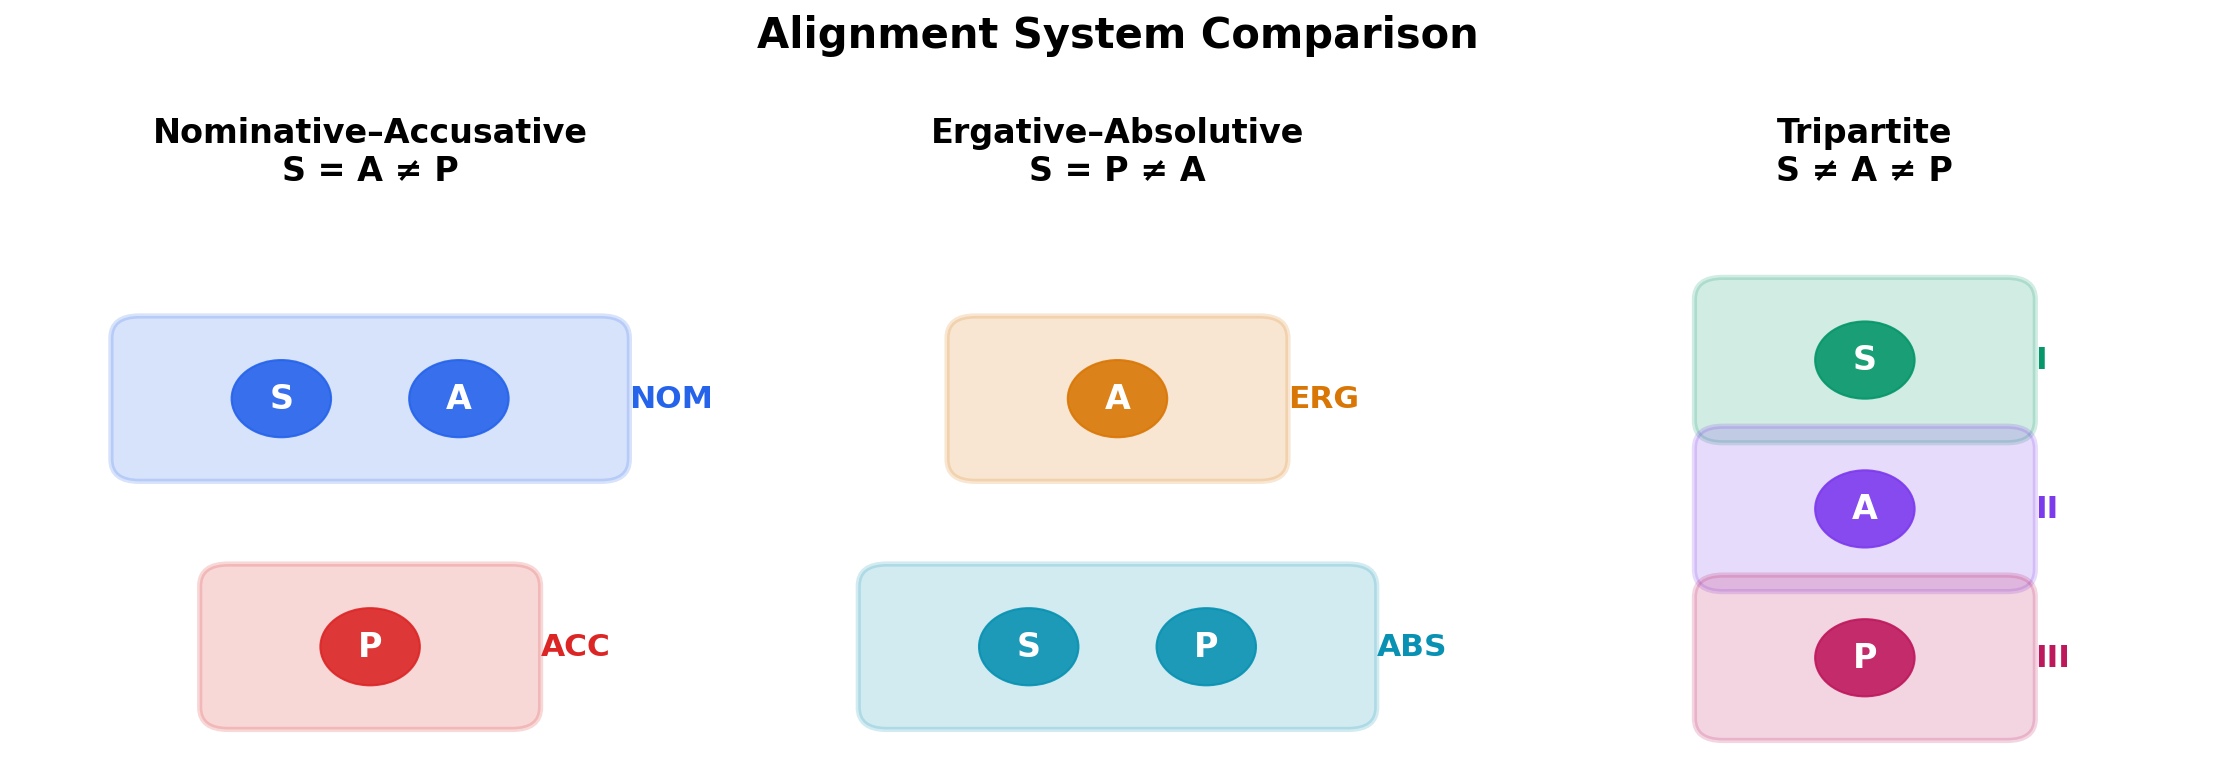
\includegraphics[keepaspectratio,alt={Side-by-side comparison of three alignment systems---Nominative-Accusative, Ergative-Absolutive, and Tripartite---showing how each alignment type groups the three core arguments (S, A, P) into distinct morphological categories. Color-coded nodes indicate case role identity; shared colors reveal the S=A or S=P neutralizations that define each alignment.}]{../figures/alignment_comparison.png}}
\caption{Side-by-side comparison of three alignment
systems---Nominative-Accusative, Ergative-Absolutive, and
Tripartite---showing how each alignment type groups the three core
arguments (S, A, P) into distinct morphological categories. Color-coded
nodes indicate case role identity; shared colors reveal the S=A or S=P
neutralizations that define each alignment.}\label{fig:alignment}
\end{figure}

\begin{figure}
\centering
\pandocbounded{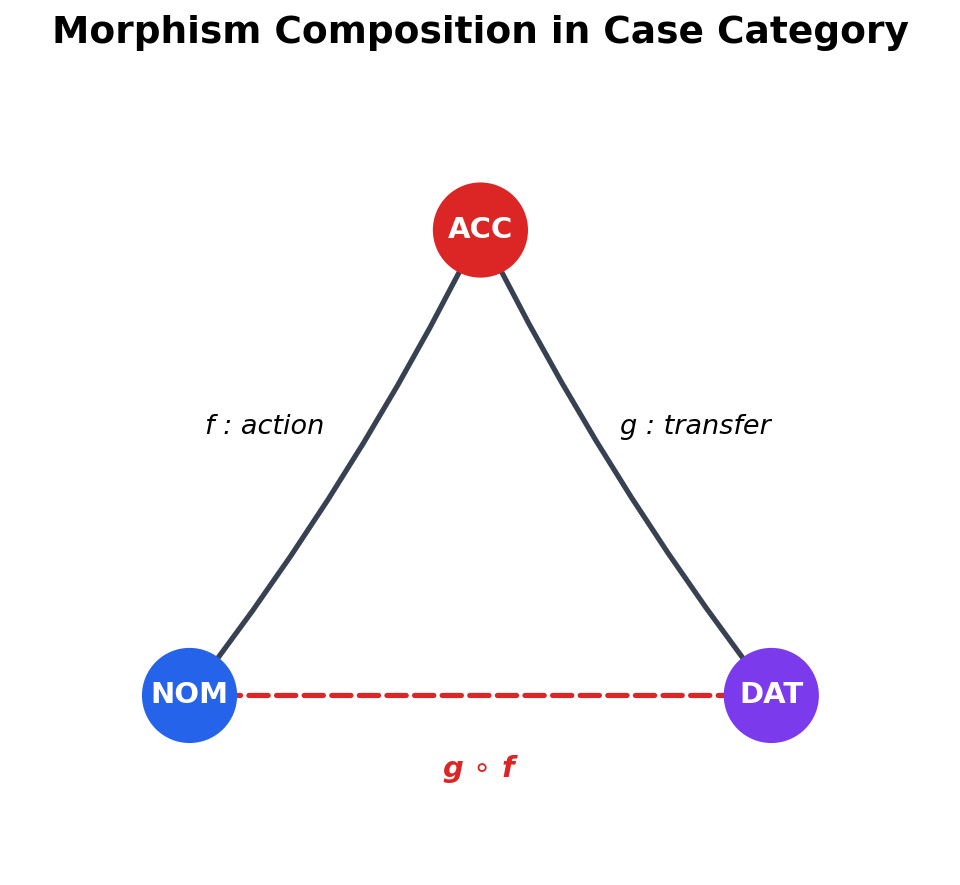
\includegraphics[keepaspectratio,alt={The categorical composition triangle: morphism f (transitive action, NOM to ACC) and morphism g (transfer, ACC to DAT) compose to yield g after f (NOM to DAT), illustrating how grammatical dependencies chain transitively through intermediate case roles. The commutativity of this triangle encodes that indirect object assignment factors through the direct object.}]{../figures/composition_triangle.png}}
\caption{The categorical composition triangle: morphism f (transitive
action, NOM to ACC) and morphism g (transfer, ACC to DAT) compose to
yield g after f (NOM to DAT), illustrating how grammatical dependencies
chain transitively through intermediate case roles. The commutativity of
this triangle encodes that indirect object assignment factors through
the direct object.}\label{fig:composition}
\end{figure}

\subsubsection{Enriched Morphisms, Proto-Roles, and Graded
Structure}\label{enriched-morphisms-proto-roles-and-graded-structure}

Following Dowty \citeyearpar{dowty1991thematic}, we equip morphisms with
weights in \([0,1]\) that encode the degree of proto-role satisfaction.
A morphism \(f: \text{NOM} \to \text{ACC}\) with weight \(w = 0.9\)
indicates a strong transitive action (clear agent acting on clear
patient), while \(w = 0.4\) might indicate an experiencer construction
(``The child fears the dark'') where the nominative argument only weakly
satisfies Proto-Agent entailments.

Composition of enriched morphisms multiplies weights:
\[w(g \circ f) = w(g) \cdot w(f) \tag{2.1}\]

This multiplicative composition reflects the intuition that grammatical
dependencies attenuate as they chain through intermediate roles.
\autoref{fig:composition} illustrates the categorical composition of two
morphisms through an intermediate case role. The resulting structure is
a category enriched over \(([0,1], \cdot, 1)\)---a connection we develop
fully in \autoref{sec:enriched-categories}.

\newpage

\section{Categorial Grammar, Pregroup Types, and String
Diagrams}\label{sec:categorial-grammar}

\subsection{From Phrase Structure Rules to Algebraic Type
Assignment}\label{from-phrase-structure-rules-to-algebraic-type-assignment}

Traditional generative grammar assigns sentence structure through
phrase-structure rules that recursively combine constituents into larger
units. Categorial grammar inverts this perspective: rather than
specifying construction rules, it assigns each lexical item a
\emph{type} that encodes its combinatory potential. A transitive verb
like ``chases'' is not described as ``a word that takes a subject NP and
an object NP to form a VP'' but rather as having the type
\((n \backslash s) / n\)---an entity that seeks a noun to its right (the
object) and a noun to its left (the subject) in order to produce a
sentence.

\subsection{Lambek's Residuated Syntactic
Calculus}\label{lambeks-residuated-syntactic-calculus}

The algebraic foundations were laid by Lambek
\citeyearpar{lambek1958mathematics}, who introduced a \emph{residuated}
structure on syntactic types: two binary operations, the left residual
\(\backslash\) and the right residual \(/\) of the multiplicative
connective \(\otimes\) (concatenation). The key axiom is the residuation
law:

\[A \otimes B \leq C \quad \iff \quad A \leq C / B \quad \iff \quad B \leq A \backslash C \tag{3.1}\]

This law captures the fundamental duality of syntax: a verb of type
\((n \backslash s) / n\) \emph{consumes} noun arguments to
\emph{produce} a sentence. The resulting \textbf{Lambek calculus} is a
non-commutative intuitionistic linear logic---non-commutative because
word order matters, and linear because each resource (word) is used
exactly once.

\subsubsection{Pregroup Grammars and Compact Closed
Structure}\label{pregroup-grammars-and-compact-closed-structure}

Lambek \citeyearpar{lambek2004fine} later simplified the framework to
\textbf{pregroup grammars}, where each type \(a\) has a left adjoint
\(a^l\) and a right adjoint \(a^r\) satisfying:

\[a^l \cdot a \leq 1 \leq a \cdot a^l \qquad a \cdot a^r \leq 1 \leq a^r \cdot a \tag{3.2}\]

This formal structuralism was revolutionized by Coecke, Sadrzadeh, and
Clark's introduction of the \textbf{DisCoCat} (Distributional
Compositional Categorical) model in 2010
\citeyearpar{coecke2010mathematical}. DisCoCat unifies categorial
grammar with distributional semantics by defining strong monoidal
functors from pregroup grammars to vector spaces. As Duneau (2021)
summarizes, ``The distributional compositional approach to modelling
meaning\ldots{} allows the meaning of a sentence to be computed as a
function of both the distributional meaning of the words involved, as
well as its grammatical form'' \citeyearpar{duneau2021parsing}. By
demonstrating that pregroups and finite-dimensional vector spaces are
both rigid monoidal categories, DisCoCat enables sentence meanings to be
computed linearly from constituent word meanings.

Grammaticality reduces to checking whether a sequence of types reduces
to the sentence type \(s\) via these \emph{contraction}
(\(a^l \cdot a \to 1\)) and \emph{expansion} (\(1 \to a \cdot a^l\))
steps. This reformulation is crucial for the DisCoCat framework
(\autoref{sec:categorical-semantics}) because pregroups form
\textbf{compact closed categories}, which have a well-developed
diagrammatic calculus.

\subsection{String Diagrams for Syntactic
Derivation}\label{string-diagrams-for-syntactic-derivation}

The pivotal connection between categorial grammar and visualization
comes from Joyal and Street \citeyearpar{joyalstreet1991geometry}, who
proved that morphisms in monoidal categories can be faithfully
represented as \emph{string diagrams}---planar graphs where:

\begin{itemize}
\tightlist
\item
  \textbf{Wires} represent types (objects of the category)
\item
  \textbf{Boxes} represent words or operations (morphisms)
\item
  \textbf{Vertical composition} represents sequential application
\item
  \textbf{Horizontal juxtaposition} represents the tensor product
  (concatenation)
\item
  \textbf{Cups and caps} represent the contraction/expansion of a
  pregroup
\end{itemize}

\autoref{fig:string-diagram} shows a DisCoCat-style string diagram for
the sentence ``Alice chases Bob,'' generated by our visualization
pipeline. The noun wires connect to the verb's input slots, and the
sentence wire emerges from the verb's output---the entire derivation
from word types to sentence type is visible at a glance.

\begin{figure}
\centering
\pandocbounded{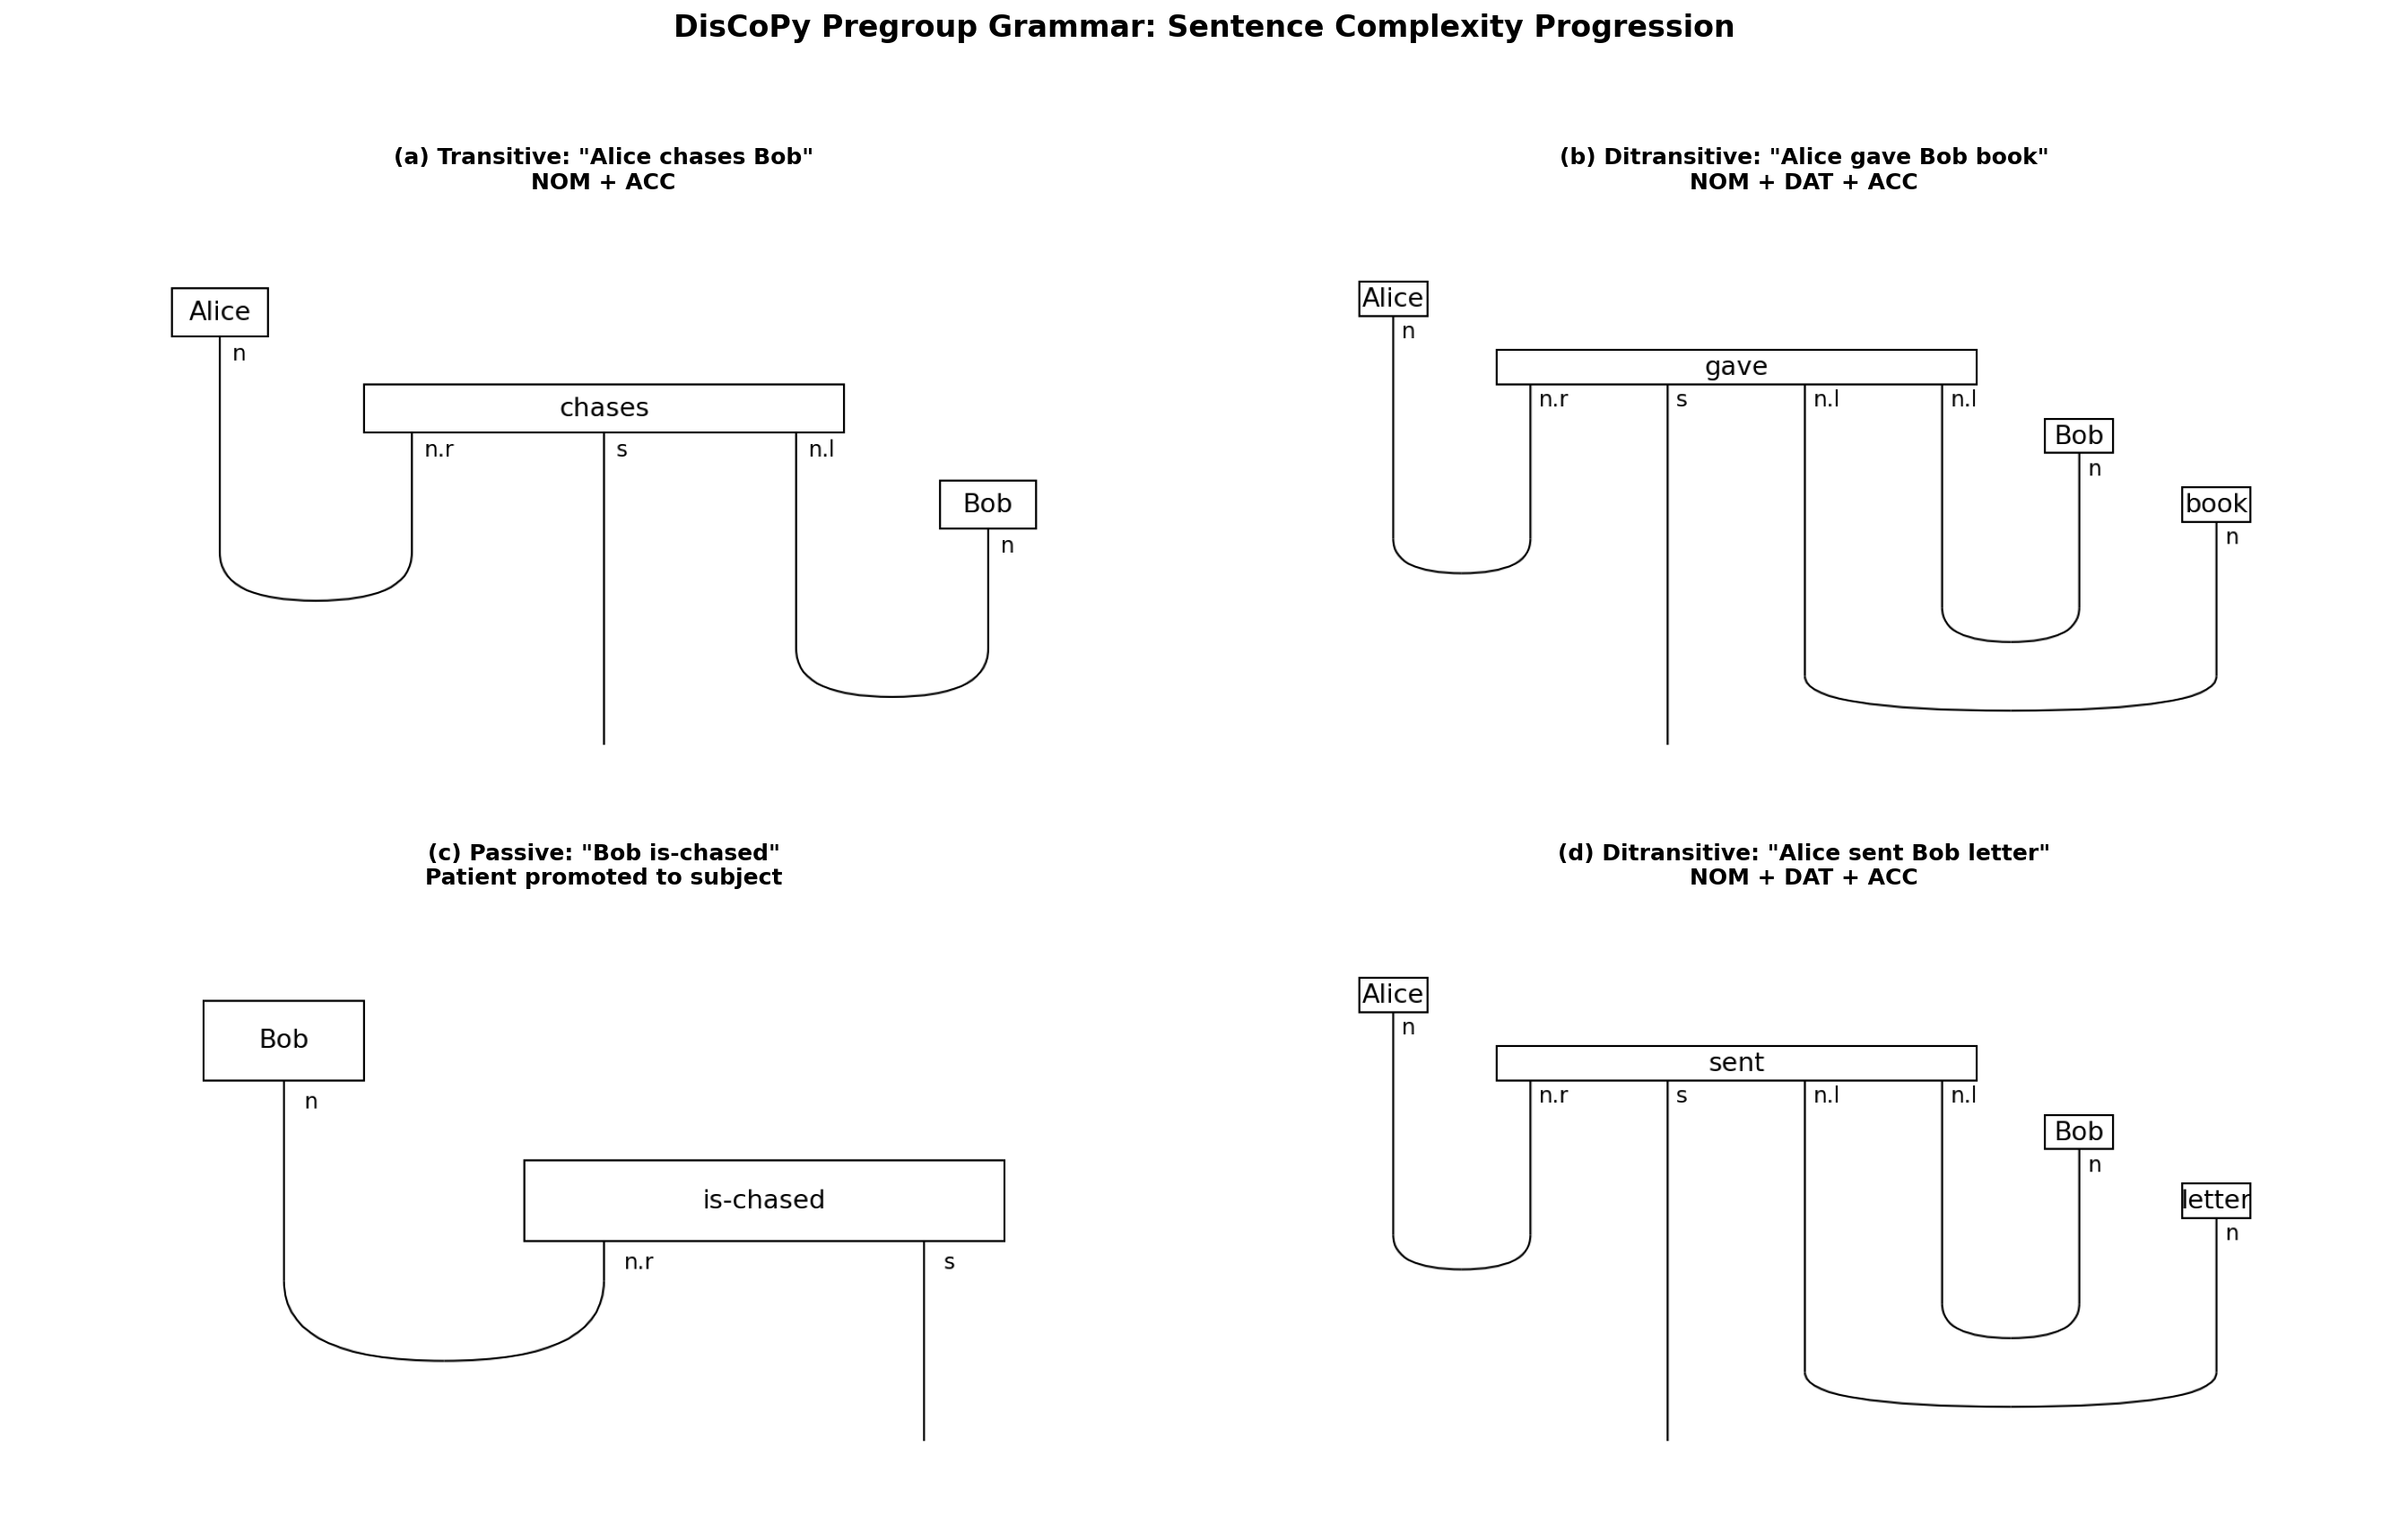
\includegraphics[keepaspectratio,alt={A 2×2 grid of DisCoPy pregroup grammar derivations showing increasing sentence complexity. Panel (a): transitive ``Alice chases Bob'' (NOM+ACC) with two cups contracting noun types into the verb. Panel (b): ditransitive ``Alice gave Bob book'' (NOM+DAT+ACC) with three cups and cascading contractions. Panel (c): passive ``Bob is-chased'' showing patient promotion to subject position via a reduced pregroup type. Panel (d): ditransitive variant ``Alice sent Bob letter'' demonstrating the same NOM+DAT+ACC pattern with different lexical items, confirming structural regularity across verbs.}]{../figures/discopy_sentence_progression.png}}
\caption{A 2×2 grid of DisCoPy pregroup grammar derivations showing
increasing sentence complexity. Panel (a): transitive ``Alice chases
Bob'' (NOM+ACC) with two cups contracting noun types into the verb.
Panel (b): ditransitive ``Alice gave Bob book'' (NOM+DAT+ACC) with three
cups and cascading contractions. Panel (c): passive ``Bob is-chased''
showing patient promotion to subject position via a reduced pregroup
type. Panel (d): ditransitive variant ``Alice sent Bob letter''
demonstrating the same NOM+DAT+ACC pattern with different lexical items,
confirming structural regularity across
verbs.}\label{fig:string-diagram}
\end{figure}

\begin{figure}
\centering
\pandocbounded{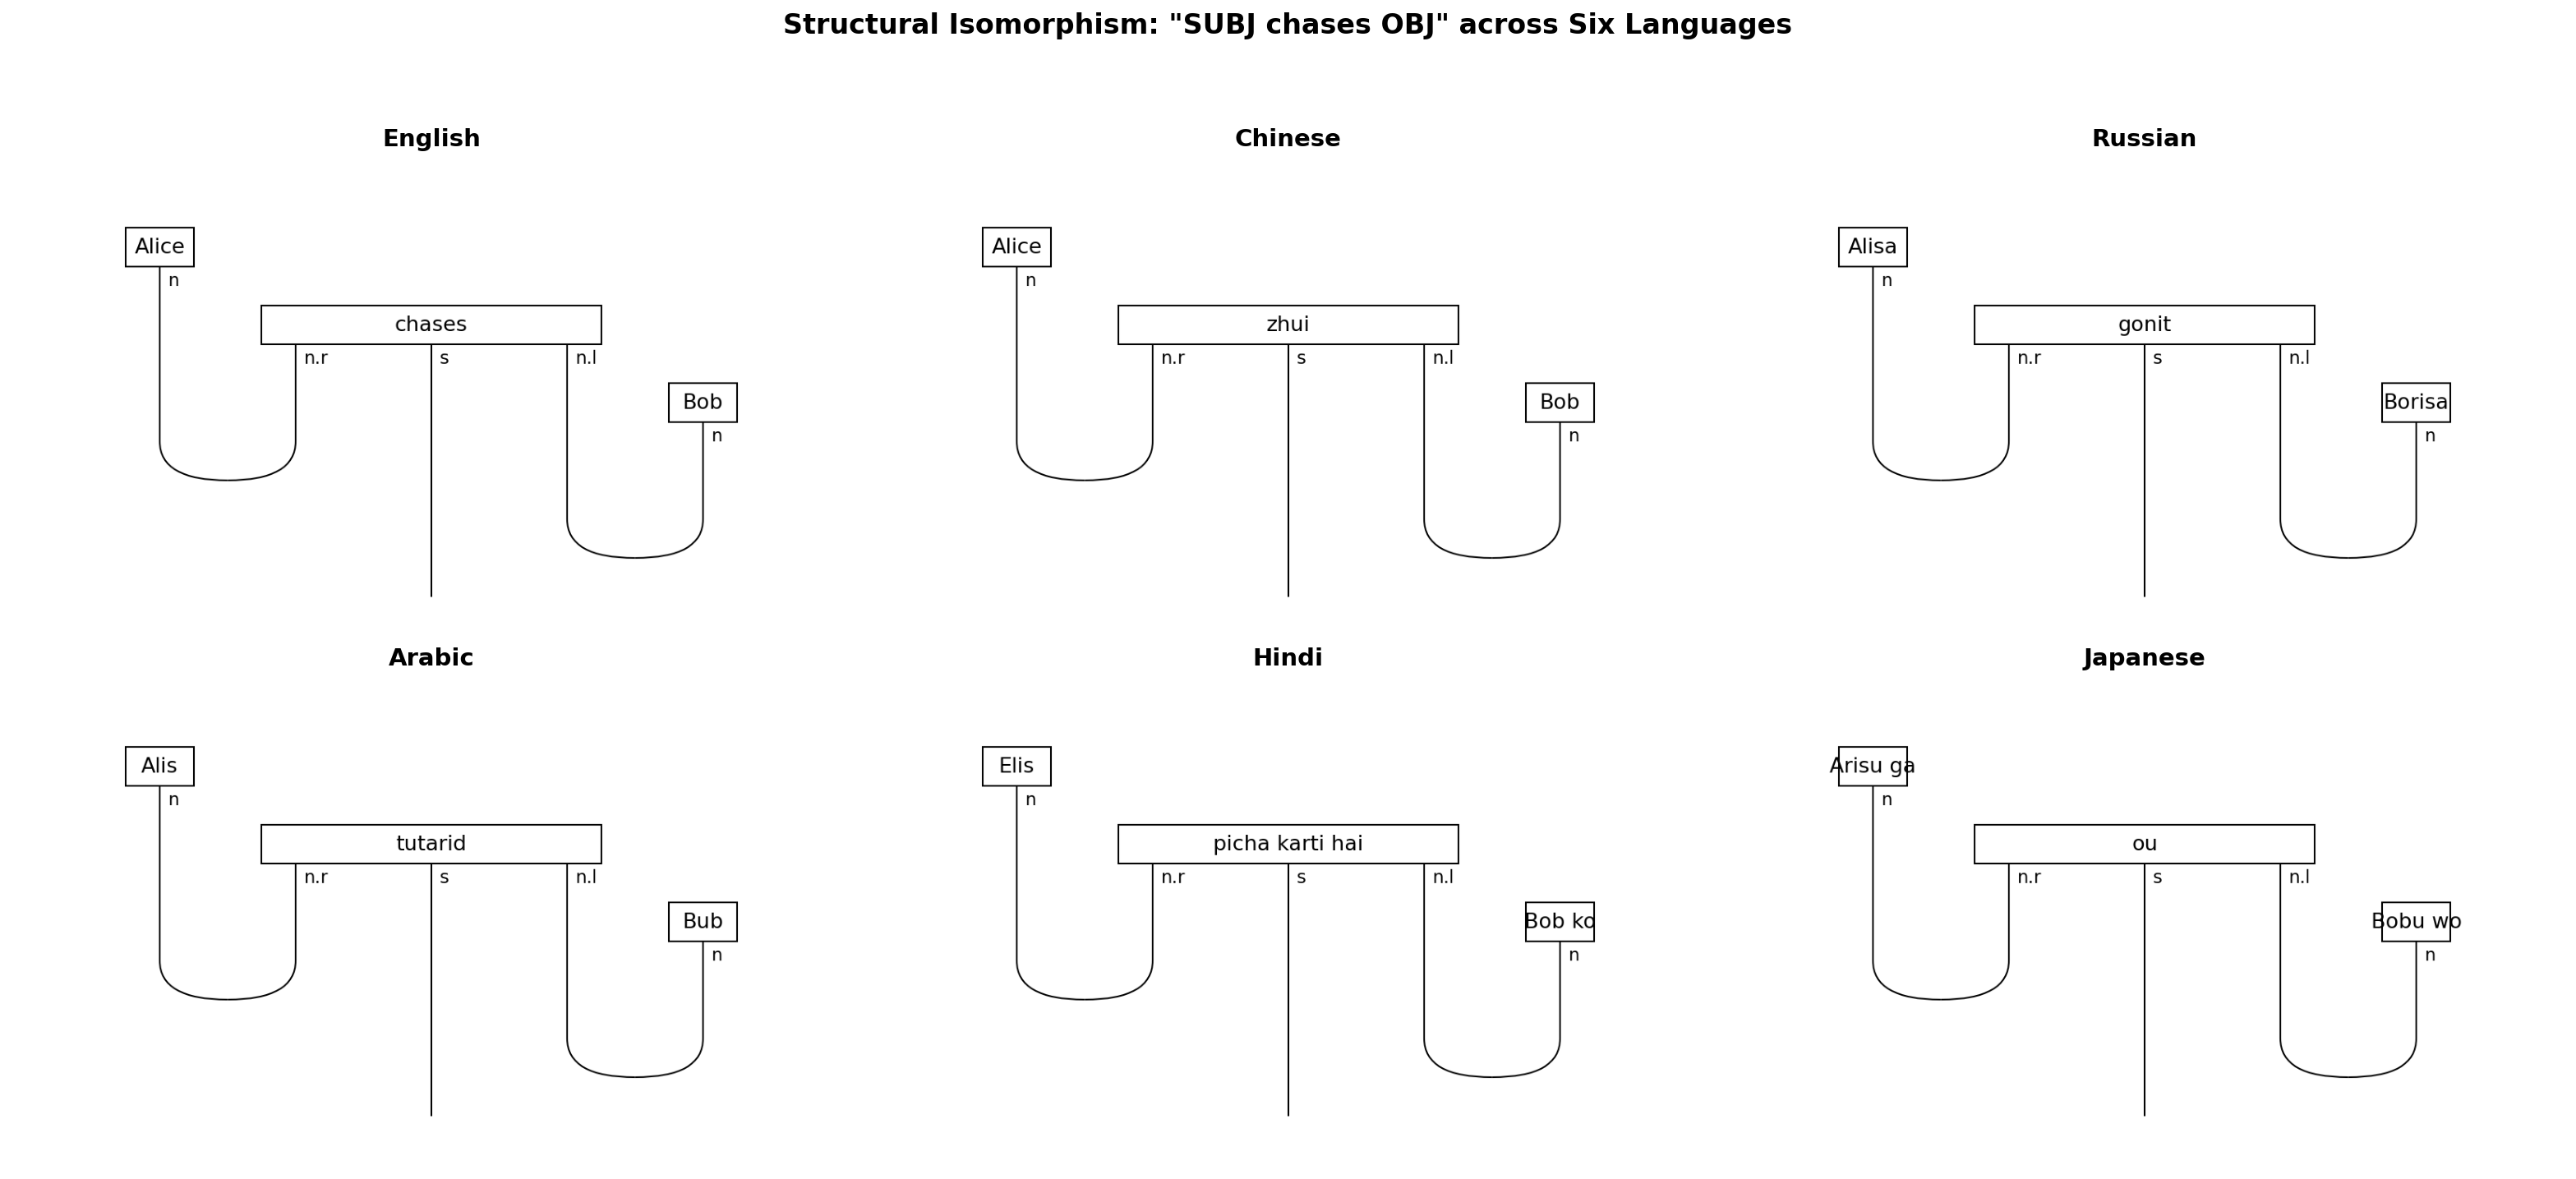
\includegraphics[keepaspectratio,alt={Structural isomorphism of pregroup grammar derivations across six languages: English, Chinese, Russian, Arabic, Hindi, and Japanese. Each panel shows the same transitive sentence (``SUBJ chases OBJ'') rendered as a DisCoPy string diagram with identical type-logical structure --- n ⊗ (n\^{}r ⊗ s ⊗ n\^{}l) ⊗ n → s --- demonstrating that the categorical type reduction is language-invariant despite surface-level morphosyntactic differences.}]{../figures/discopy_multilingual.png}}
\caption{Structural isomorphism of pregroup grammar derivations across
six languages: English, Chinese, Russian, Arabic, Hindi, and Japanese.
Each panel shows the same transitive sentence (``SUBJ chases OBJ'')
rendered as a DisCoPy string diagram with identical type-logical
structure --- n ⊗ (n\^{}r ⊗ s ⊗ n\^{}l) ⊗ n → s --- demonstrating that
the categorical type reduction is language-invariant despite
surface-level morphosyntactic
differences.}\label{fig:multilingual-isomorphism}
\end{figure}

The \emph{soundness and completeness} of string-diagrammatic reasoning
(Joyal--Street theorem) guarantees that any conclusion drawn from the
diagram is algebraically valid.

This visual transparency is precisely the ``free ride'' phenomenon
identified by Shimojima \citeyearpar{shimojima1996reasoning}: the
diagram simultaneously represents the syntactic derivation, the argument
structure, and the compositional flow of meaning, without requiring
explicit inference steps to relate them.

\begin{figure}
\centering
\pandocbounded{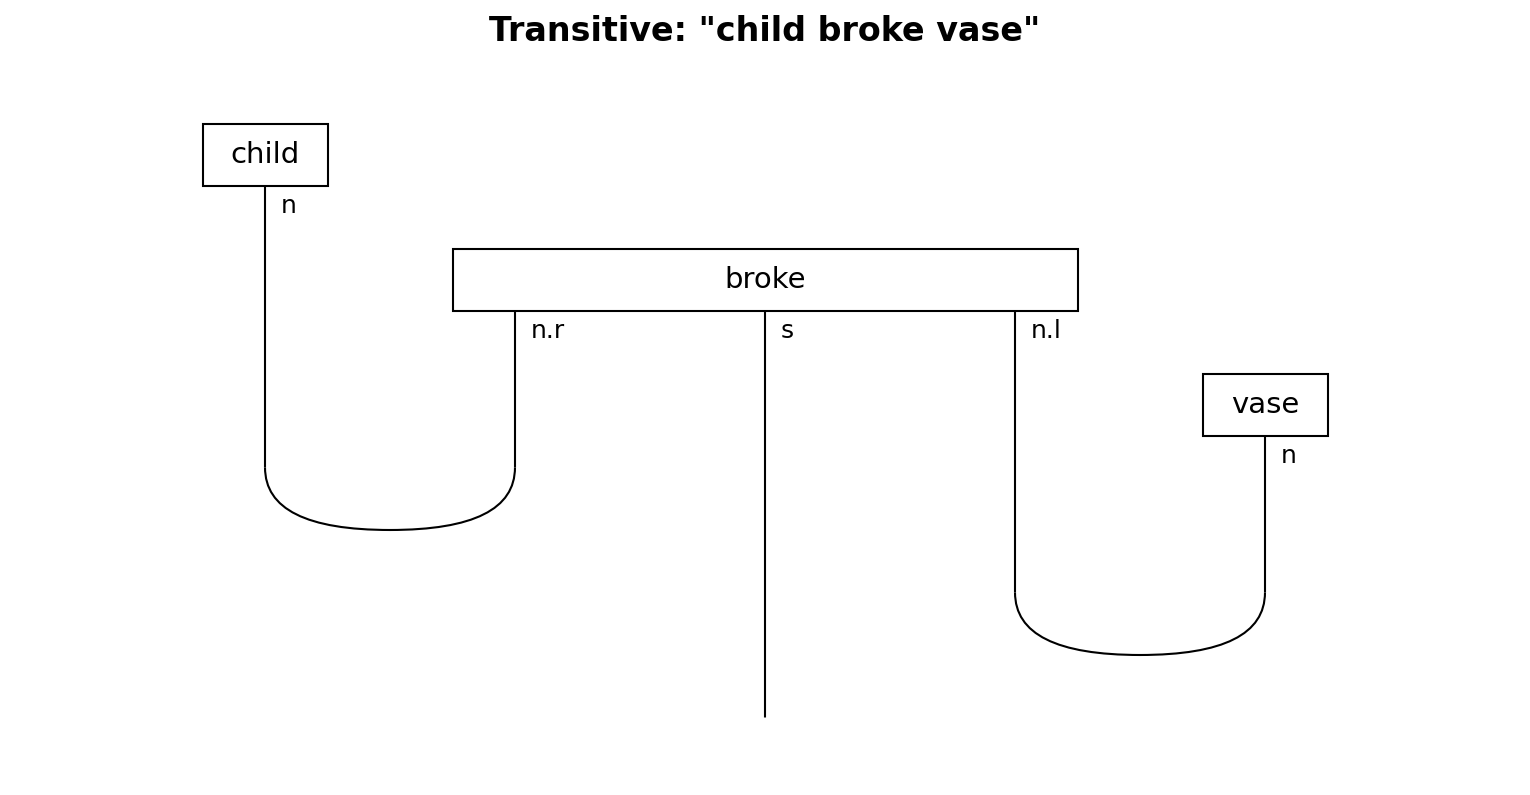
\includegraphics[keepaspectratio,alt={DisCoPy-rendered pregroup grammar diagram for the transitive sentence ``child broke vase,'' produced by the DisCoPy library's native drawing backend. The three Word boxes (child type n, broke type n.r @ s @ n.l, vase type n) are connected by Cup contractions---the leftward cup cancels n with n.r and the rightward cup cancels n.l with n---reducing the entire expression to the sentence type s. The diagrammatic structure makes the type-theoretic derivation immediately inspectable.}]{../figures/discopy_transitive.png}}
\caption{DisCoPy-rendered pregroup grammar diagram for the transitive
sentence ``child broke vase,'' produced by the DisCoPy library's native
drawing backend. The three Word boxes (child type n, broke type n.r @ s
@ n.l, vase type n) are connected by Cup contractions---the leftward cup
cancels n with n.r and the rightward cup cancels n.l with n---reducing
the entire expression to the sentence type s. The diagrammatic structure
makes the type-theoretic derivation immediately
inspectable.}\label{fig:discopy-transitive}
\end{figure}

\subsection{Case Marking in Type-Logical Categorial
Grammar}\label{case-marking-in-type-logical-categorial-grammar}

Case-marked noun phrases receive compound types that encode both their
grammatical role and their combinatory potential. In a
nominative--accusative language, we can assign:

{\def\LTcaptype{none} % do not increment counter
\begin{longtable}[]{@{}
  >{\raggedright\arraybackslash}p{(\linewidth - 4\tabcolsep) * \real{0.3333}}
  >{\raggedright\arraybackslash}p{(\linewidth - 4\tabcolsep) * \real{0.3333}}
  >{\raggedright\arraybackslash}p{(\linewidth - 4\tabcolsep) * \real{0.3333}}@{}}
\toprule\noalign{}
\begin{minipage}[b]{\linewidth}\raggedright
Expression
\end{minipage} & \begin{minipage}[b]{\linewidth}\raggedright
Type
\end{minipage} & \begin{minipage}[b]{\linewidth}\raggedright
Gloss
\end{minipage} \\
\midrule\noalign{}
\endhead
\bottomrule\noalign{}
\endlastfoot
``Alice'' (subject) & \(n_{\text{NOM}}\) & Noun, nominative-marked \\
``the ball'' (object) & \(n_{\text{ACC}}\) & Noun, accusative-marked \\
``kicks'' & \((n_{\text{NOM}} \backslash s) / n_{\text{ACC}}\) & Seeks
ACC right, NOM left \\
``to Bob'' (recipient) & \((s \backslash s) / n_{\text{DAT}}\) &
Modifies sentence via DAT argument \\
\end{longtable}
}

The subscripts refine the basic noun type \(n\) with case features,
ensuring that ``kicks'' selects a nominative subject and an accusative
object. Mismatch in case features blocks the derivation, modeling
ungrammaticality.

\subsection{The Curry--Howard Correspondence and Proof-Theoretic
Semantics}\label{the-curryhoward-correspondence-and-proof-theoretic-semantics}

A deep structural parallel underlies the Lambek calculus: derivations of
syntactic types correspond to proofs in intuitionistic logic (via the
Curry--Howard isomorphism), and therefore to programs in a typed lambda
calculus. Specifically:

{\def\LTcaptype{none} % do not increment counter
\begin{longtable}[]{@{}
  >{\raggedright\arraybackslash}p{(\linewidth - 4\tabcolsep) * \real{0.3333}}
  >{\raggedright\arraybackslash}p{(\linewidth - 4\tabcolsep) * \real{0.3333}}
  >{\raggedright\arraybackslash}p{(\linewidth - 4\tabcolsep) * \real{0.3333}}@{}}
\toprule\noalign{}
\begin{minipage}[b]{\linewidth}\raggedright
Syntactic Domain
\end{minipage} & \begin{minipage}[b]{\linewidth}\raggedright
Logical Domain
\end{minipage} & \begin{minipage}[b]{\linewidth}\raggedright
Computational Domain
\end{minipage} \\
\midrule\noalign{}
\endhead
\bottomrule\noalign{}
\endlastfoot
Types \((A / B, A \backslash B)\) & Propositions & Types \\
Derivations & Proofs & Programs (\(\lambda)\text{-terms}) \\
Cut elimination & Proof normalization & \(\beta)-reduction \\
Commutativity of cuts & Confluence of rewriting & Church--Rosser
property \\
\end{longtable}
}

This correspondence has two important consequences for our framework:

\begin{enumerate}
\def\labelenumi{\arabic{enumi}.}
\item
  \textbf{Semantic compositionality follows from syntactic
  well-formedness}: a well-typed derivation automatically yields a
  well-formed meaning representation (the \(\lambda)\text{-term}
  extracted from the proof).
\item
  \textbf{Case assignment is type inference}: determining the case of a
  noun phrase in context is equivalent to inferring the type of a
  variable in a \(\lambda)\text{-expression}---a computational problem
  with well-understood algorithms.
\end{enumerate}

\subsection{Monadic Semantics for Sublexical Root
Syntax}\label{monadic-semantics-for-sublexical-root-syntax}

Song \citetext{\citeyear{song2022act}; \citeyear{song2022blog}} extends
the categorial framework with a \textbf{monadic semantics} for root
syntax, modeling the sublexical decomposition of verb roots using monads
in a syntactic category. This approach captures the intuition that a
verb like ``break'' has internal compositional structure---a causative
layer and a result-state layer---that interacts with case assignment.
The monad encapsulates the complexity of root meaning within a single
categorical construction, allowing the type-logical grammar to handle
both lexical and syntactic composition uniformly.

The monadic approach connects naturally to graded type theory: Asudeh
and Giorgolo \citeyearpar{asudeh2020graded} develop a monadic semantics
for evidentiality that uses graded effects to track the epistemic status
of propositions---a pattern that extends to case, where the ``grade'' of
a morphism could encode the strength of a semantic role assignment.

\subsection{Passivization as Algebraic Type
Permutation}\label{passivization-as-algebraic-type-permutation}

One of the most revealing case-theoretic operations is
\textbf{passivization}, which transforms an active transitive clause
into a passive construction by promoting the patient to subject position
and (optionally) demoting the agent to an oblique role. In our
categorical framework, passivization is not an ad hoc syntactic
transformation but a precise \emph{type permutation}---a swap of the
noun types feeding into the verb's pregroup derivation.

In a pregroup grammar, the active transitive ``Alice chases Bob'' has
the type reduction:

\[n_{\text{NOM}} \cdot (n^r \cdot s \cdot n^l) \cdot n_{\text{ACC}} \to s \tag{3.3}\]

Passivization permutes the noun arguments, yielding ``Bob is chased by
Alice'' with the swapped type assignment:

\[n_{\text{ACC}} \cdot (n^r \cdot s \cdot n^l) \cdot n_{\text{NOM}} \to s \tag{3.4}\]

Crucially, DisCoPy's \texttt{Swap} primitive makes this permutation
explicit and algebraically precise: the swap operation
\(\sigma_{n,n}: n \otimes n \to n \otimes n\) permutes the two noun
wires without violating the monoidal structure. The resulting diagram
differs from the active version precisely in the crossing of the noun
wires---making the voice alternation \emph{visible} as a topological
feature of the string diagram.

This diagrammatic transparency exemplifies Shimojima's
\citeyearpar{shimojima1996reasoning} free-ride inference: by inspecting
the diagram, one can immediately see that passivization preserves the
verb's inherent argument structure while rearranging the surface
realization---a fact that requires multiple inference steps to establish
in a linear notation.

\begin{figure}
\centering
\pandocbounded{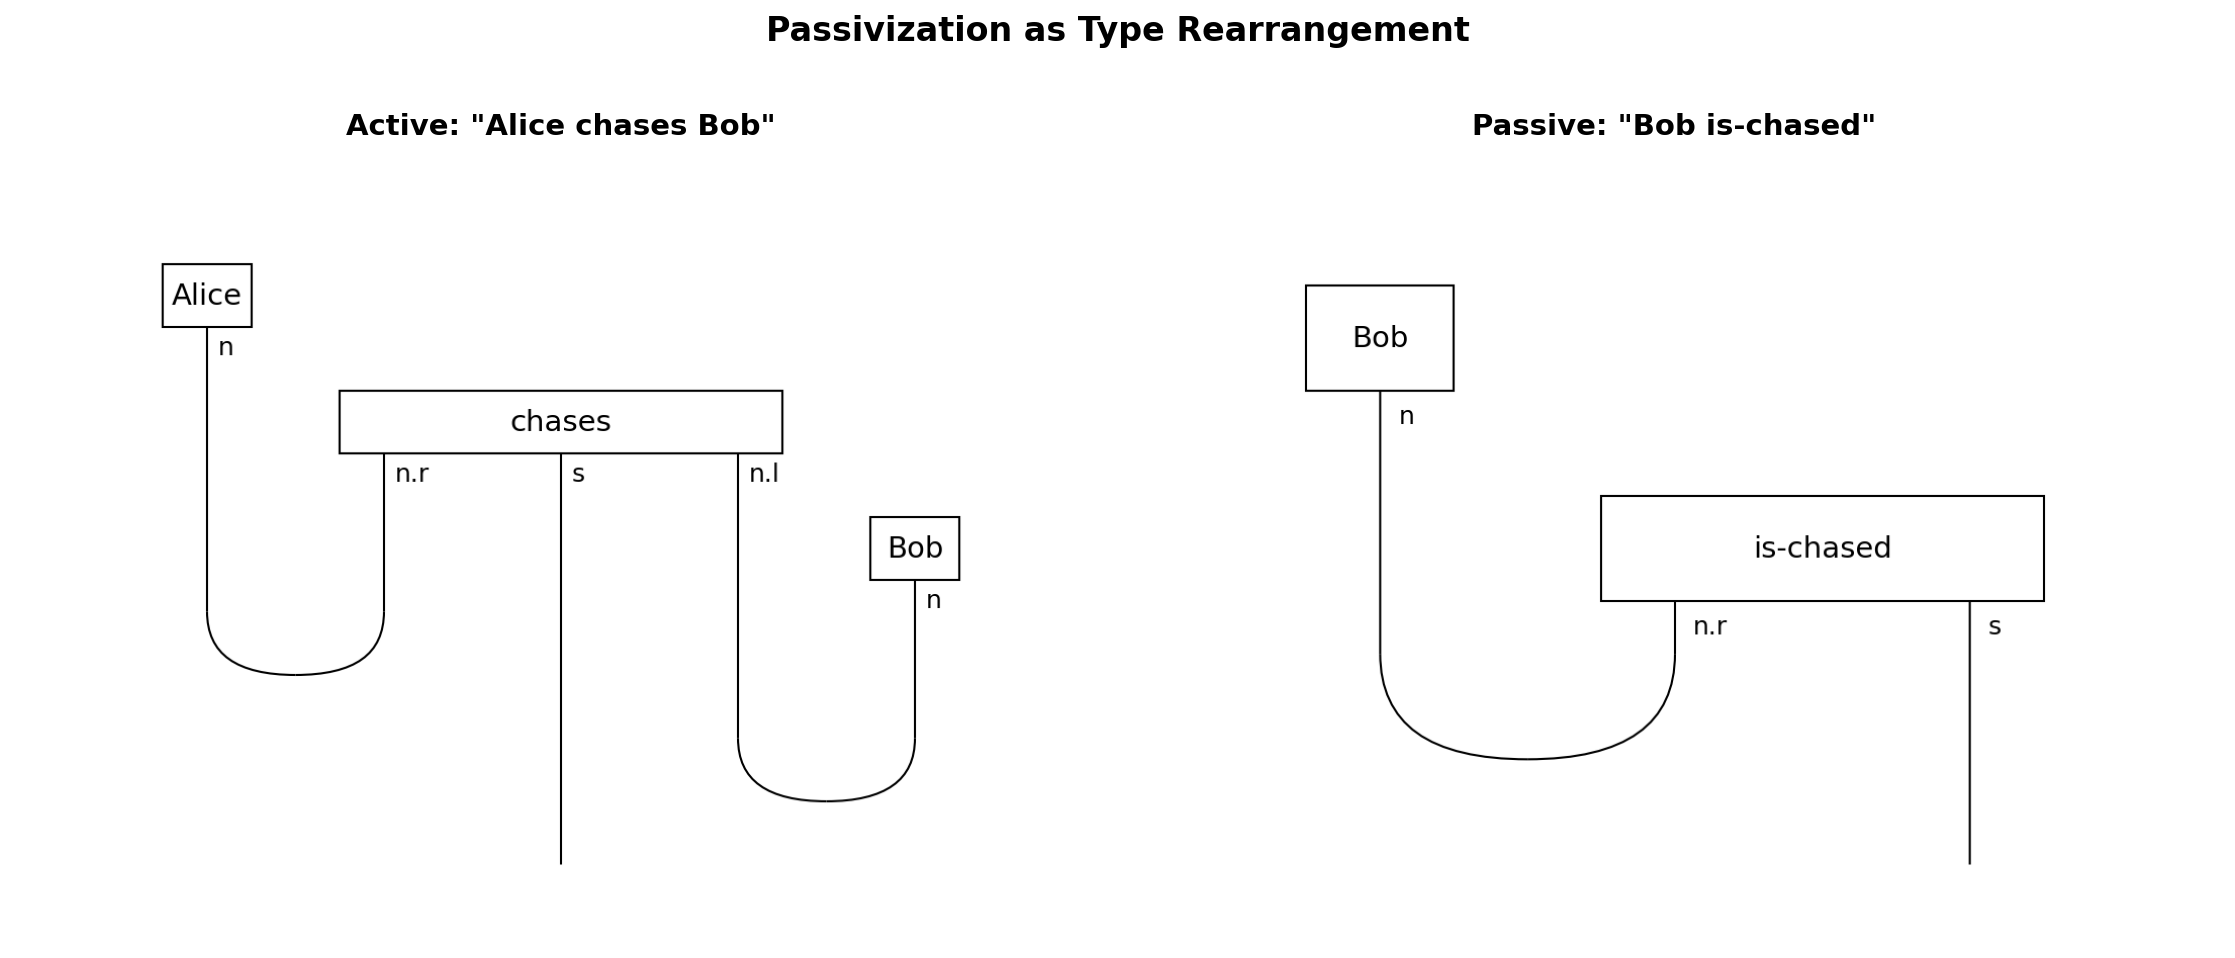
\includegraphics[keepaspectratio,alt={Passivization modeled as a type permutation: the active transitive sentence ``Alice chases Bob'' (left panel) and its passive counterpart ``Bob is-chased'' (right panel), both rendered by DisCoPy. In the active diagram, nom-type Alice feeds the verb's n.r slot while acc-type Bob feeds n.l; in the passive, the patient Bob is promoted to subject (n) position while the verb's type reduces to n.r @ s. The structural difference between voice alternations is visible as a topological change in the wire connectivity.}]{../figures/discopy_passive.png}}
\caption{Passivization modeled as a type permutation: the active
transitive sentence ``Alice chases Bob'' (left panel) and its passive
counterpart ``Bob is-chased'' (right panel), both rendered by DisCoPy.
In the active diagram, nom-type Alice feeds the verb's n.r slot while
acc-type Bob feeds n.l; in the passive, the patient Bob is promoted to
subject (n) position while the verb's type reduces to n.r @ s. The
structural difference between voice alternations is visible as a
topological change in the wire connectivity.}\label{fig:discopy-passive}
\end{figure}

\newpage

\section{Categorical Compositional Distributional Semantics
(DisCoCat)}\label{sec:categorical-semantics}

\subsection{Two Traditions of Meaning: Formal and
Distributional}\label{two-traditions-of-meaning-formal-and-distributional}

The study of linguistic meaning has long been divided between two
traditions with complementary strengths and weaknesses:

\begin{enumerate}
\def\labelenumi{\arabic{enumi}.}
\item
  \textbf{Formal semantics}, following Montague
  \citeyearpar{montague1973proper}, assigns meaning compositionally: the
  meaning of a complex expression is a function of the meanings of its
  parts and the way they are syntactically combined. This tradition
  excels at capturing logical structure (quantification, negation,
  modality) but struggles with lexical meaning---it typically treats
  content words as unanalyzed primitives.
\item
  \textbf{Distributional semantics} assigns meaning empirically: a
  word's meaning is characterized by its distribution across contexts,
  typically encoded as a vector in a high-dimensional space. The
  distributional hypothesis---``You shall know a word by the company it
  keeps'' \citep{firth1957papers}---traces to J.R. Firth's contextual
  theory of meaning and, independently, to Zellig Harris's
  \citeyearpar{harris1954distributional} algebraic analysis of
  distributional structure, which demonstrated that linguistic elements
  occurring in similar environments share semantic properties. This
  tradition captures graded similarity and analogy but lacks
  compositional structure---the meaning of ``dog bites man'' and ``man
  bites dog'' may receive identical vector representations.
\end{enumerate}

The tension between these two traditions is one of the deepest in the
science of language. Turney and Pantel's
\citeyearpar{turney2010frequency} comprehensive survey of vector space
models showed that distributional methods capture remarkably
fine-grained semantic distinctions---synonymy, antonymy, hypernymy,
analogy---but only at the word level. Baroni and Lenci
\citeyearpar{baroni2010distributional} developed a tensor-based
\emph{Distributional Memory} framework that partially addresses
compositionality by structuring co-occurrence data as a three-way tensor
over (word, relation, word) triples, but without a principled
type-logical backbone. Lenci \citeyearpar{lenci2018distributional}
surveys the modern landscape and identifies the central open problem:
how to reconcile the \emph{algebraic compositionality} of formal
semantics with the \emph{empirical grounding} of distributional models.

The \textbf{DisCoCat} (Distributional Compositional Categorical)
framework \citep{coecke2010mathematical} resolves this tension by using
category theory to compose distributional meanings according to
syntactic structure---achieving, for the first time, a framework that is
simultaneously \emph{compositional} (from categorial grammar),
\emph{distributional} (from corpus-derived vector spaces), and
\emph{algebraically principled} (from monoidal category theory).

\subsection{From Static Embeddings to Contextual Representations: LLMs
as Distributional
Models}\label{from-static-embeddings-to-contextual-representations-llms-as-distributional-models}

The distributional programme has undergone a dramatic computational
intensification in the era of large language models (LLMs). The
trajectory from classical co-occurrence matrices through static word
embeddings to contextual transformers can be understood as a progressive
\emph{enrichment} of the distributional hypothesis itself:

\begin{enumerate}
\def\labelenumi{\arabic{enumi}.}
\item
  \textbf{Static embeddings}: Mikolov et al.'s
  \citeyearpar{mikolov2013efficient} Word2Vec (skip-gram and CBOW
  architectures) demonstrated that prediction-based training on local
  context windows produces word vectors exhibiting striking algebraic
  regularity---the famous ``king \(-\) man \(+\) woman \(\approx\)
  queen'' analogy. Pennington et al.'s \citeyearpar{pennington2014glove}
  GloVe incorporated global co-occurrence statistics via log-bilinear
  regression, yielding vectors whose inner products approximate
  pointwise mutual information. Both models instantiate the
  distributional hypothesis in its classical Firthian form: meaning is
  determined by context of use, encoded as geometric position in a
  learned vector space.
\item
  \textbf{Contextual embeddings}: BERT \citep{devlin2019bert} and GPT
  \citep{radford2018improving} move beyond static type-level
  representations to \emph{token-level} contextualized embeddings, where
  the same word receives different vectors in different contexts. In the
  terms of the formal/distributional dichotomy, this is a critical
  advance: contextualized embeddings partially capture
  \emph{compositional} structure by conditioning word representations on
  their full sentential environment, resolving polysemy and
  constructional effects that static embeddings conflate.
\item
  \textbf{Transformer architecture}: The transformer
  \citep{vaswani2017attention} implements distributional composition
  through multi-head self-attention, where each attention head computes
  a weighted combination of input token representations. The attention
  weights \(\alpha_{ij} = \text{softmax}(Q_i K_j^T / \sqrt{d_k})\) are
  analogous to the enriched hom-values of
  \autoref{sec:enriched-categories}: they encode the \emph{degree of
  contextual relevance} between tokens \(i\) and \(j\) in a given
  representational subspace---a graded, learned distributional relation.
\end{enumerate}

The connection to our categorical framework is direct: \textbf{DisCoCat
is the algebraic formalization of what LLMs do empirically.} Where a
transformer computes sentence representations by attending to
syntactically and semantically relevant tokens through learned weight
matrices, DisCoCat composes word vectors through type-logical
derivations in a compact closed category. The functor
\(F: \mathbf{Preg} \to \mathbf{FVect}\) that defines DisCoCat is, in
this light, the \emph{principled version} of the composition that
attention mechanisms learn from data. This perspective is confirmed by
Gavranović's \citeyearpar{gavranovic2024thesis} categorical deep
learning programme, which shows that attention heads can be understood
as parameterized optics---categorical constructions that compose
functorially, just as DisCoCat derivations do.

For case theory specifically, the transformer analogy is illuminating:
each attention head in a transformer can be understood as learning a
particular \emph{relational role}---attending to subjects, objects,
modifiers, or other grammatical functions. This is precisely the role
that case marking plays in natural language: structuring
who-does-what-to-whom. The case-typed noun spaces of our enriched
DisCoCat model
(\(N_{\text{NOM}}, N_{\text{ACC}}, N_{\text{DAT}}, \ldots\)) correspond
to the role-specific representational subspaces that different attention
heads learn to inhabit.

\subsection{The DisCoCat Compositional
Framework}\label{the-discocat-compositional-framework}

\subsubsection{The Key Insight: Shared Compact Closed
Structure}\label{the-key-insight-shared-compact-closed-structure}

DisCoCat's central observation is that pregroup grammars and vector
spaces share a common abstract structure: both are \textbf{compact
closed categories}. This means there exists a \emph{meaning functor}:

\[F: \mathbf{Preg} \to \mathbf{FVect} \tag{4.1}\]

from the pregroup grammar category (where objects are types and
morphisms are grammatical reductions) to the category of
finite-dimensional vector spaces (where objects are vector spaces and
morphisms are linear maps).

Under this functor:

\begin{itemize}
\tightlist
\item
  Noun types \(n\) map to a vector space \(N\) (the noun space)
\item
  Sentence types \(s\) map to a vector space \(S\) (the sentence space)
\item
  A transitive verb of type \(n^r \cdot s \cdot n^l\) maps to a tensor
  in \(N \otimes S \otimes N\)
\item
  Pregroup contractions (cups/caps) map to the standard inner product
  and its dual
\end{itemize}

\subsubsection{Computing Compositional Sentence
Meaning}\label{computing-compositional-sentence-meaning}

The compositional meaning of a sentence is computed by tensoring the
word meanings and then contracting the result along the indices
determined by the syntactic derivation. For ``Alice chases Bob'':

\[\overrightarrow{\text{Alice chases Bob}} = (\overrightarrow{\text{Alice}} \otimes \overleftrightarrow{\text{chases}} \otimes \overrightarrow{\text{Bob}}) \circ (\varepsilon_N \otimes 1_S \otimes \varepsilon_N) \tag{4.2}\]

where \(\varepsilon_N: N \otimes N \to \mathbb{R}\) is the compact
closure map (inner product). This computation has a direct diagrammatic
representation as a string diagram---the same Joyal--Street
\citep{joyalstreet1991geometry} formalism that governs the syntax.

\subsubsection{Empirical Validation and
Disambiguation}\label{empirical-validation-and-disambiguation}

Grefenstette and Sadrzadeh \citeyearpar{grefenstette2015concrete}
demonstrated that DisCoCat models can outperform purely distributional
baselines on disambiguation and sentence similarity tasks. The key
advantage is that compositional structure resolves ambiguities that
bag-of-words models cannot: ``dog bites man'' and ``man bites dog''
receive different sentence vectors because the syntactic structure
assigns different roles to the nouns.

\begin{figure}
\centering
\pandocbounded{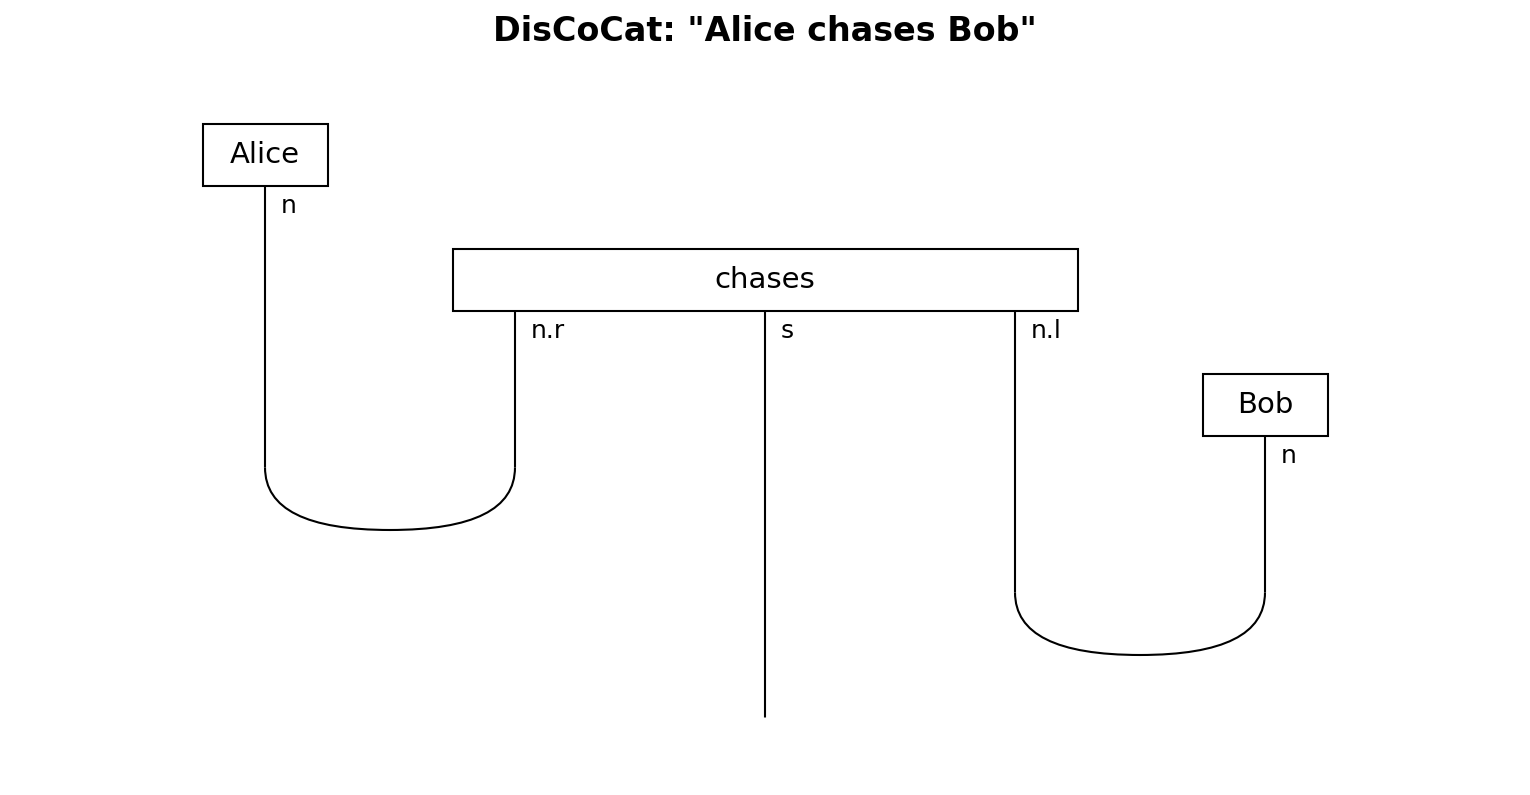
\includegraphics[keepaspectratio,alt={DisCoPy rendering of the DisCoCat sentence ``Alice chases Bob'' as a pregroup grammar string diagram, produced using the DisCoPy library's native drawing backend. The three Word boxes (Alice type n, chases type n.r @ s @ n.l, Bob type n) are connected by Cup contractions that cancel adjoint type pairs, reducing the entire expression to the sentence type s. This demonstrates the monoidal structure of type contraction that underlies all DisCoCat computations.}]{../figures/discopy_discocat.png}}
\caption{DisCoPy rendering of the DisCoCat sentence ``Alice chases Bob''
as a pregroup grammar string diagram, produced using the DisCoPy
library's native drawing backend. The three Word boxes (Alice type n,
chases type n.r @ s @ n.l, Bob type n) are connected by Cup contractions
that cancel adjoint type pairs, reducing the entire expression to the
sentence type s. This demonstrates the monoidal structure of type
contraction that underlies all DisCoCat
computations.}\label{fig:discopy-discocat}
\end{figure}

\subsection{Case Enrichment in the DisCoCat
Framework}\label{case-enrichment-in-the-discocat-framework}

The present contribution lies in showing how case marking enriches the
DisCoCat framework with explicit role structure. In a case-marked
DisCoCat model:

\begin{enumerate}
\def\labelenumi{\arabic{enumi}.}
\item
  \textbf{Typed noun spaces}: Instead of a single noun space \(N\), we
  define case-specific spaces
  \(N_{\text{NOM}}, N_{\text{ACC}}, N_{\text{DAT}}, \ldots\) Morphisms
  between these spaces encode case-changing operations (passivization,
  dative shift, etc.).
\item
  \textbf{Case-constrained composition}: The meaning functor \(F\) maps
  case-typed pregroup derivations to tensor contractions that respect
  case constraints. A verb seeking a nominative subject and accusative
  object contracts only with vectors from the appropriate spaces.
\item
  \textbf{Alignment as functor}: Cross-linguistic alignment differences
  correspond to different meaning functors. An accusative-language
  functor maps S and A arguments to the same noun space
  \(N_{\text{NOM}}\); an ergative-language functor maps S and P to a
  shared \(N_{\text{ABS}}\).
\end{enumerate}

\begin{figure}
\centering
\pandocbounded{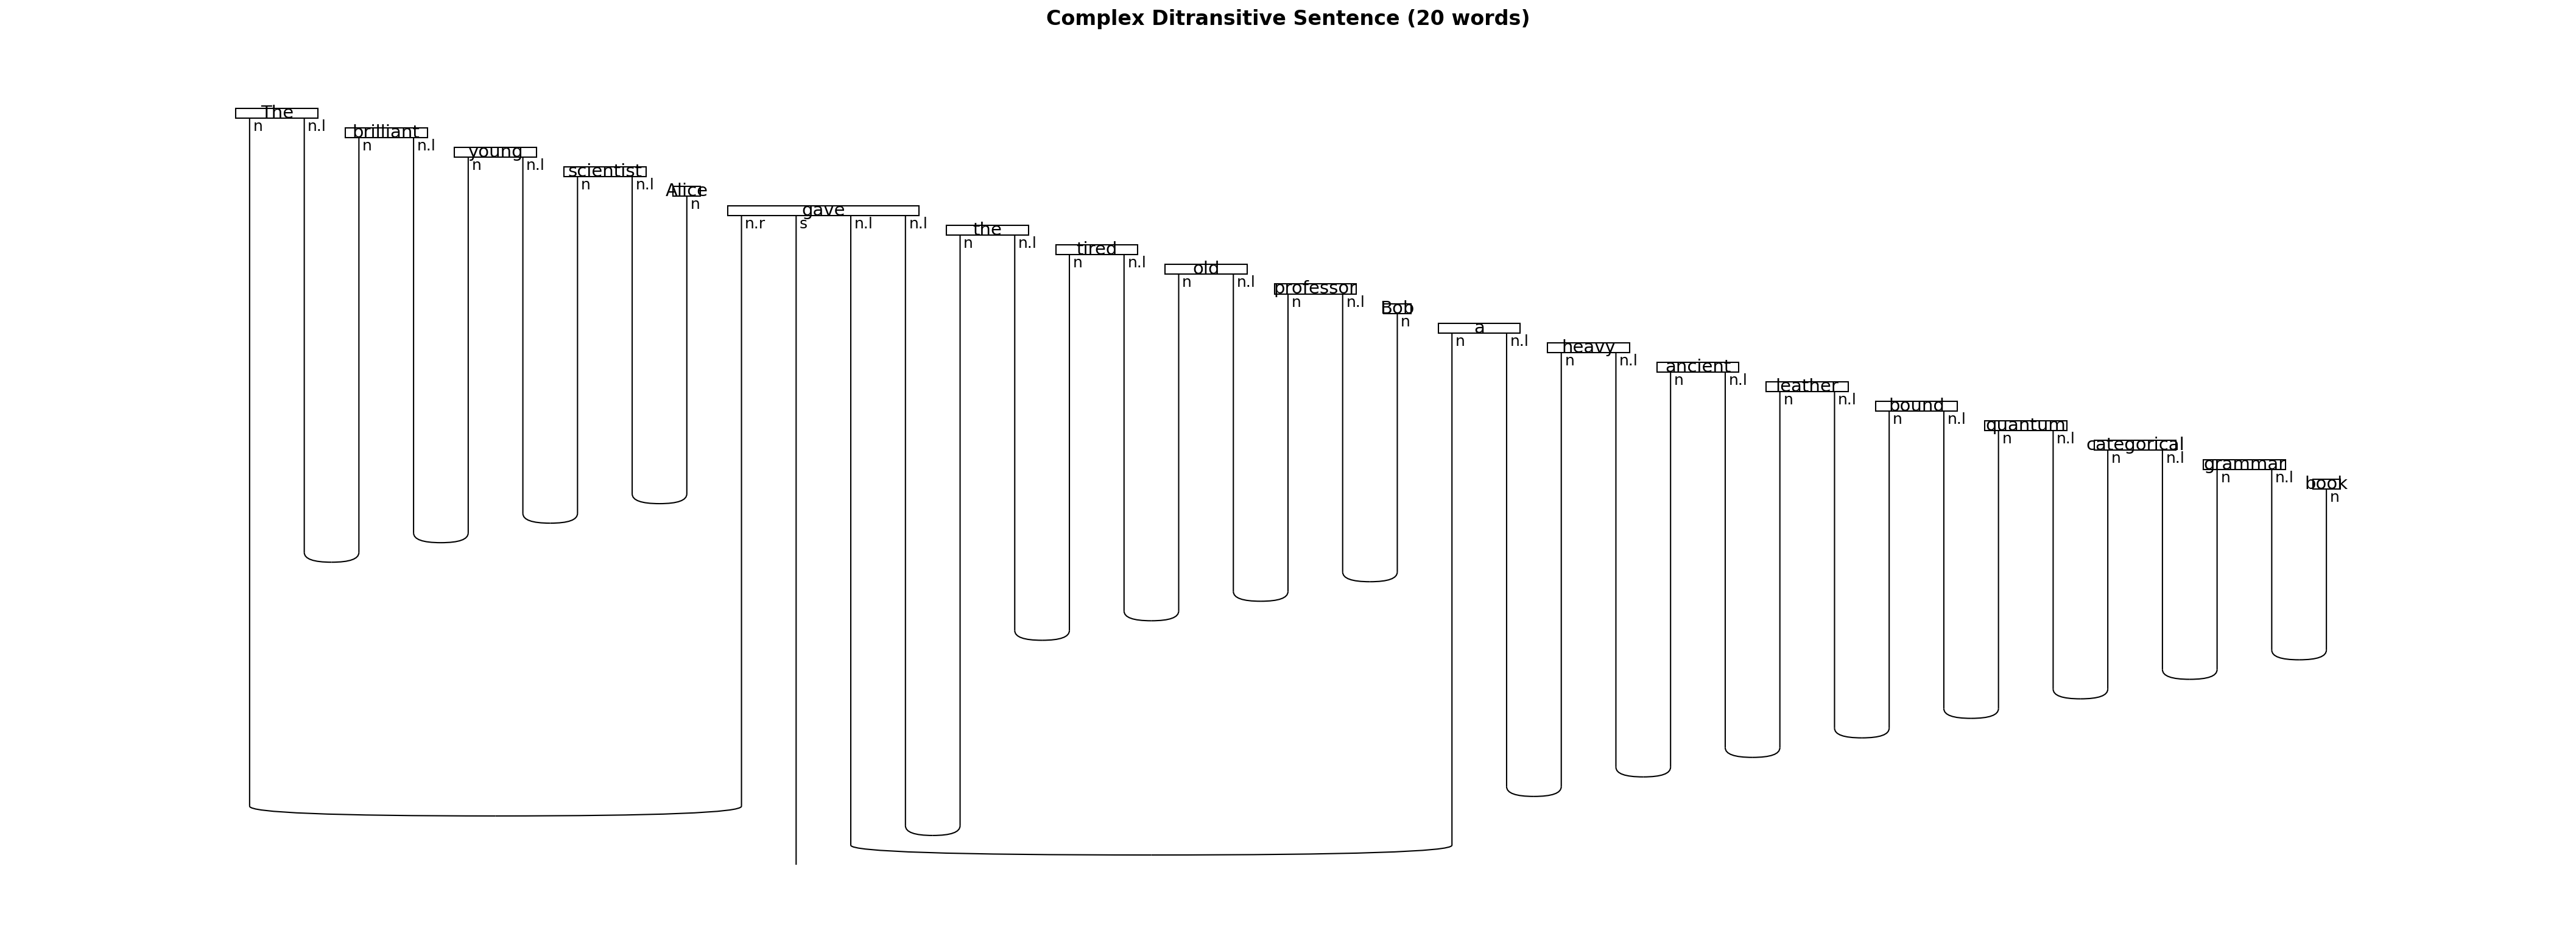
\includegraphics[keepaspectratio,alt={A massive 20-word DisCoPy pregroup grammar diagram for the complex ditransitive sentence ``The brilliant young scientist Alice gave the tired old professor Bob a heavy ancient leather bound quantum categorical grammar book.'' Generated entirely using DisCoPy's Python library, this tensor network demonstrates the combinatorial scalability of categorical compositional semantics. The diagram features three dense noun phrases (with 4, 4, and 8 chained adjective modifiers respectively), all reducing perfectly into the central verb's pregroup type n\^{}r \textbackslash otimes s \textbackslash otimes n\^{}l \textbackslash otimes n\^{}l. This single rigorous diagram maps 20 lexical items into a unified semantic type s, proving the empirical viability of string-diagrammatic grammar for complex natural language structures.}]{../figures/discopy_complex_sentence.png}}
\caption{A massive 20-word DisCoPy pregroup grammar diagram for the
complex ditransitive sentence ``The brilliant young scientist Alice gave
the tired old professor Bob a heavy ancient leather bound quantum
categorical grammar book.'' Generated entirely using DisCoPy's Python
library, this tensor network demonstrates the combinatorial scalability
of categorical compositional semantics. The diagram features three dense
noun phrases (with 4, 4, and 8 chained adjective modifiers
respectively), all reducing perfectly into the central verb's pregroup
type \(n^r \otimes s \otimes n^l \otimes n^l\). This single rigorous
diagram maps 20 lexical items into a unified semantic type \(s\),
proving the empirical viability of string-diagrammatic grammar for
complex natural language structures.}\label{fig:discopy-ditransitive}
\end{figure}

\subsection{The Compact Closure Axiom and Diagrammatic Complexity
Metrics}\label{the-compact-closure-axiom-and-diagrammatic-complexity-metrics}

\subsubsection{The Snake Equation (Zigzag
Identity)}\label{the-snake-equation-zigzag-identity}

The algebraic engine of DisCoCat is the \textbf{compact closure} of the
pregroup category: for every type \(n\), the adjunction maps
\(\eta_n: 1 \to n \otimes n^r\) (cap) and
\(\varepsilon_n: n^r \otimes n \to 1\) (cup) satisfy the \textbf{snake
equation} (also called the zigzag identity):

\[(\varepsilon_n \otimes 1_n) \circ (1_n \otimes \eta_n) = 1_n \tag{4.3}\]

In string-diagrammatic terms, a cup composed with a cap on adjacent
wires ``straightens out'' into an identity wire---a zigzag that cancels
into a straight line. This axiom is not merely a formal curiosity: it is
the \emph{engine} that makes pregroup type reductions work. Every
grammatical contraction (noun canceling with verb argument) is an
instance of the cup map \(\varepsilon\), and every expansion
(introducing an adjoint pair) is an instance of the cap map \(\eta).
The snake equation guarantees that these contractions and expansions are
well-behaved---they can be freely inserted and removed without changing
the meaning of the derivation.

The cognitive significance of the snake equation is that it provides a
\emph{visual proof} of coherence: an agent inspecting a string diagram
can verify that the derivation is well-formed by checking that all
zigzags cancel---a spatial operation that requires no algebraic
computation. This is precisely Shimojima's
\citeyearpar{shimojima1996reasoning} ``free ride'' in its purest form.

\begin{figure}
\centering
\pandocbounded{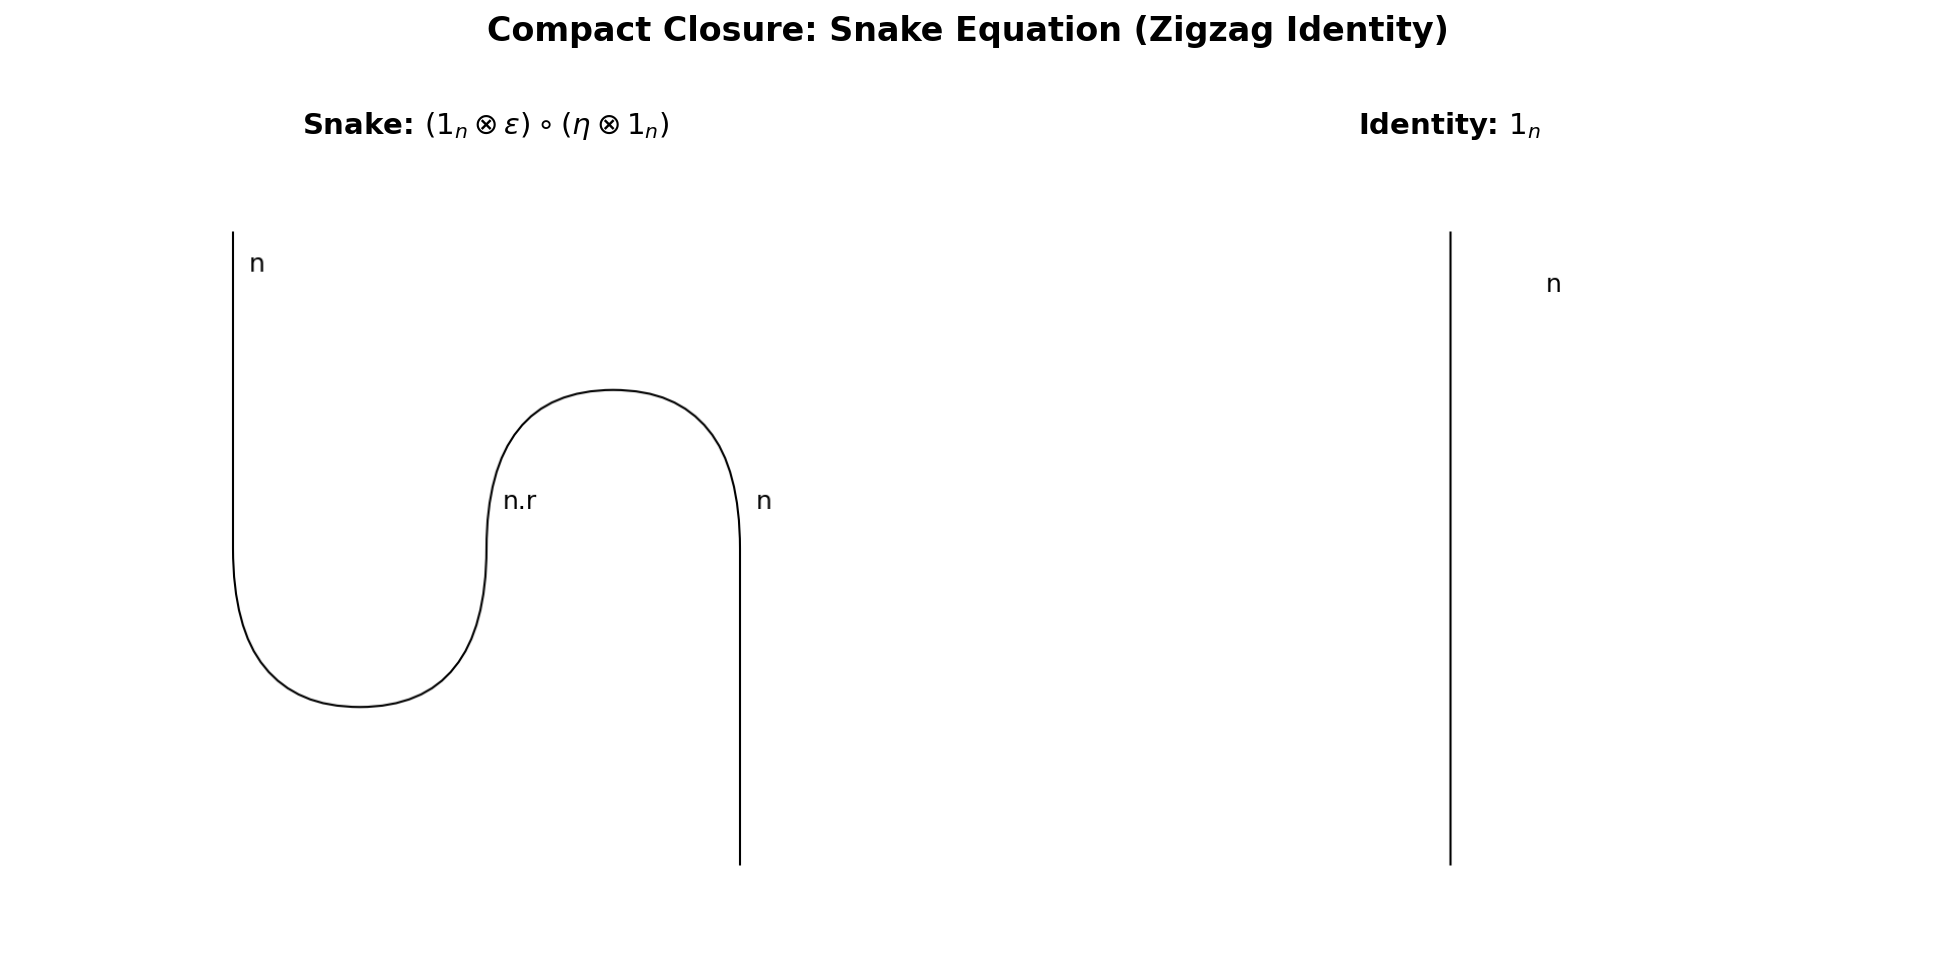
\includegraphics[keepaspectratio,alt={The snake equation (compact closure axiom) rendered by DisCoPy: the left panel shows the ``snake'' diagram where a Cup contraction (epsilon) composed with a Cap expansion (eta) on adjacent wires forms a zigzag; the right panel shows the identity wire it equals. This identity---that the zigzag straightens out---is the algebraic engine powering all pregroup type reductions and justifies the cancellation steps in every DisCoCat derivation.}]{../figures/discopy_snake.png}}
\caption{The snake equation (compact closure axiom) rendered by DisCoPy:
the left panel shows the ``snake'' diagram where a Cup contraction
(epsilon) composed with a Cap expansion (eta) on adjacent wires forms a
zigzag; the right panel shows the identity wire it equals. This
identity---that the zigzag straightens out---is the algebraic engine
powering all pregroup type reductions and justifies the cancellation
steps in every DisCoCat derivation.}\label{fig:discopy-snake}
\end{figure}

\subsubsection{Diagram Complexity Metrics: Normal Form and
Depth}\label{diagram-complexity-metrics-normal-form-and-depth}

The algebraic properties of pregroup diagrams support quantitative
analysis of derivational complexity. Two measures are particularly
informative:

\begin{enumerate}
\def\labelenumi{\arabic{enumi}.}
\item
  \textbf{Normal form}: A diagram is in \emph{normal form} if no further
  simplifications (zigzag cancellations, box reordering) are possible.
  The \texttt{normal\_form()} operation computes this canonical
  representative of the diagram's equivalence class.
\item
  \textbf{Depth}: The \emph{depth} of a diagram is the length of the
  longest path from input to output, counting boxes. Deeper diagrams
  encode more complex syntactic derivations---a ditransitive sentence
  like ``Alice gave Bob a book'' (depth 7) is structurally more complex
  than a simple intransitive ``Alice runs'' (depth 3).
\end{enumerate}

These metrics connect to the enriched framework of
\autoref{sec:enriched-categories}: the depth of a DisCoCat derivation
diagram can serve as a proxy for the syntactic complexity component of
the enriched hom-value, providing a principled bridge between the
type-logical and distributional perspectives on linguistic structure.

\subsection{Extensions: From Sentence Meaning to Discourse
Coherence}\label{extensions-from-sentence-meaning-to-discourse-coherence}

\subsubsection{DisCoCirc: Distributional Compositional
Circuits}\label{discocirc-distributional-compositional-circuits}

The original DisCoCat framework operates at the sentence level: each
sentence receives a vector meaning, but there is no mechanism for
tracking how meanings interact across sentences. De Felice and Coecke
\citeyearpar{defelice2020discourse} address this with \textbf{DisCoCirc}
(Distributional Compositional Circuits), which extends the categorical
framework to handle discourse-level semantic structure.

DisCoCirc introduces \emph{state wires} that persist across sentence
boundaries, encoding the evolving states of discourse entities
(characters, objects, topics). A sentence like ``Alice chased Bob. He
was terrified.'' is represented as a circuit where:

\begin{itemize}
\tightlist
\item
  Alice and Bob are wires that persist across both sentences
\item
  The pronoun ``He'' is resolved by connecting its wire to Bob's wire
\item
  The emotional state ``terrified'' updates the state information
  carried by Bob's wire
\end{itemize}

De Felice et al. \citeyearpar{defelice2022discocirc} further develop
this into a full-fledged circuit model that handles ambiguity,
coreference, and discourse coherence within the same categorical
formalism. A CCG-based pipeline for generating discourse circuits from
syntactic parse trees has recently demonstrated that DisCoCirc can scale
to real-world text, dynamically composing sentence-level diagrams along
shared entity wires via an iterative process of coreference resolution
and wire merging \citeyearpar{duneau2021parsing}. Complementary work on
\textbf{DiscoSG} (Discourse Scene Graphs) extends this approach to
multi-sentence image captions, parsing text into scene graphs that
capture cross-sentence coreference relations. \autoref{fig:discourse}
illustrates a multi-sentence discourse diagram where entity wires
persist across sentence boundaries. For case theory, DisCoCirc is
significant because it shows how case-marked argument structure
\emph{composes across discourse}: the nominative subject of one sentence
can become the accusative object of the next, and this transformation is
tracked as a morphism in the discourse category.

\begin{figure}
\centering
\pandocbounded{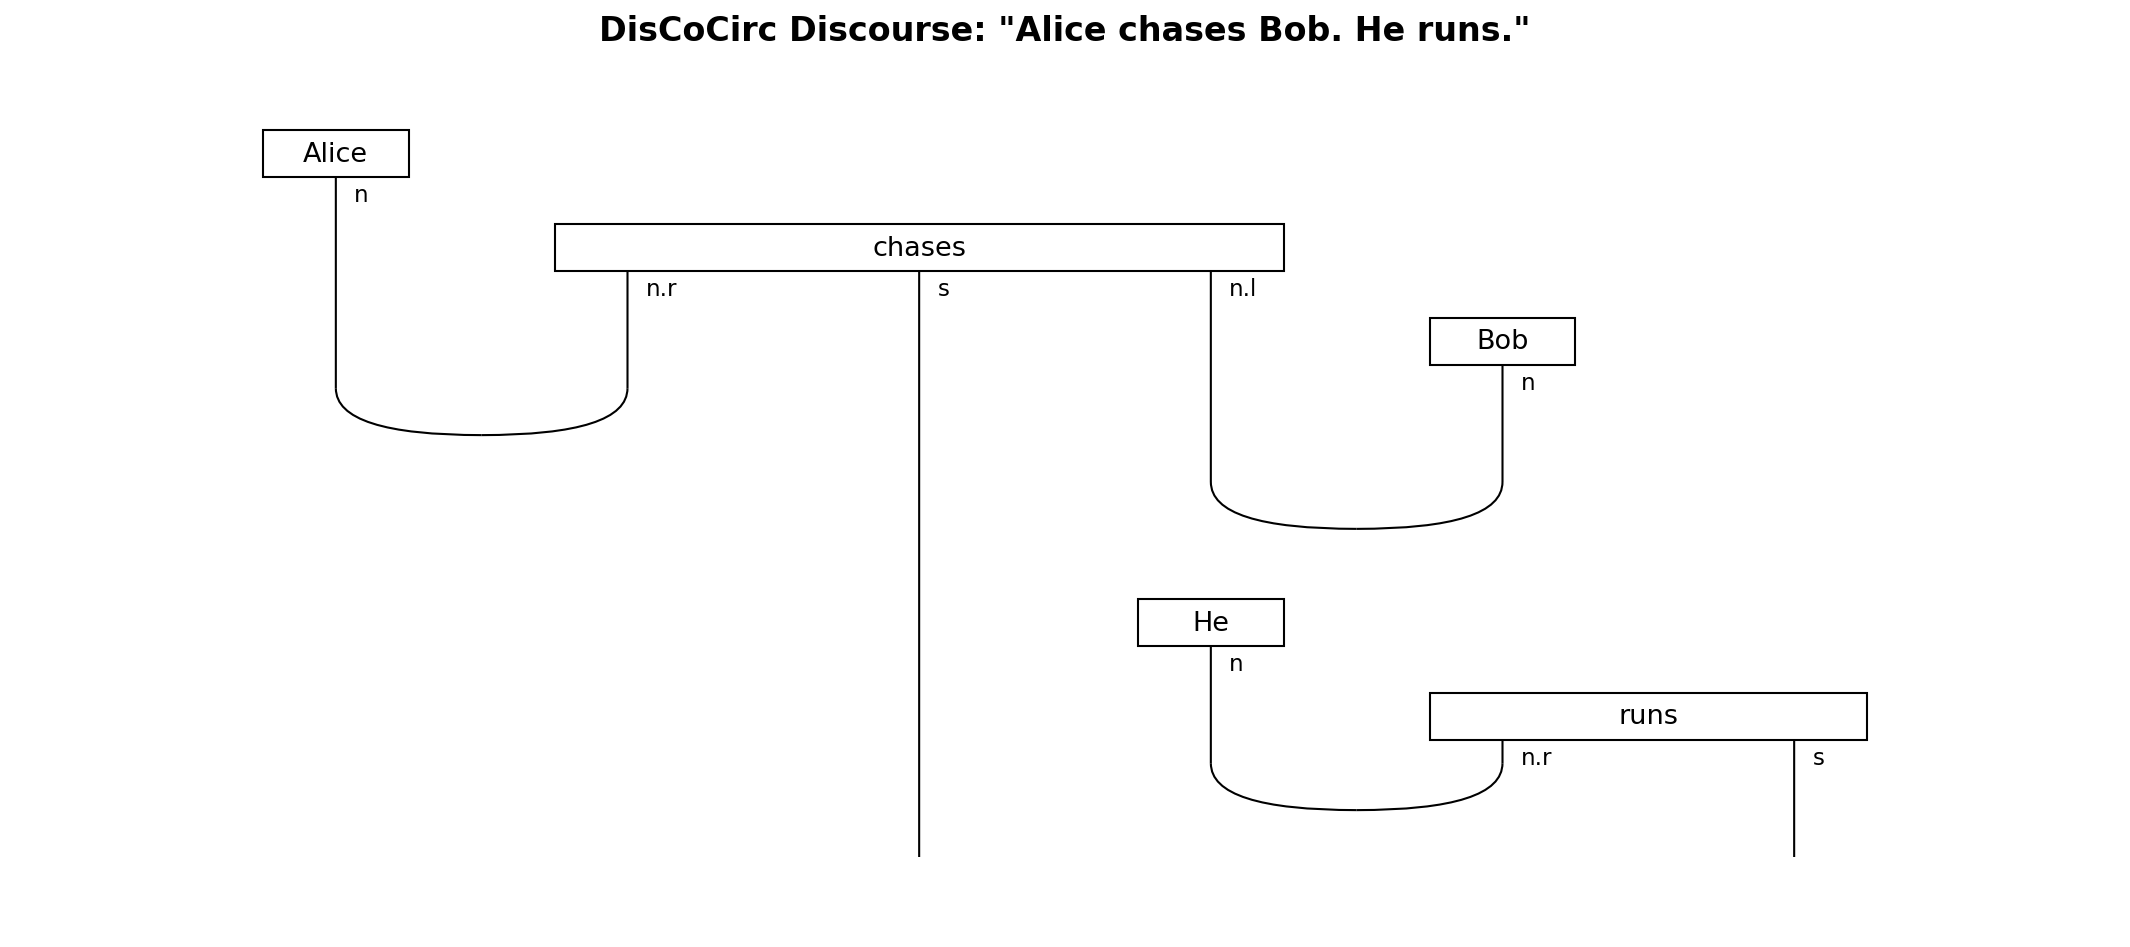
\includegraphics[keepaspectratio,alt={A DisCoCirc-style discourse diagram for the two-sentence discourse ``Alice chases Bob. Bob runs,'' generated using DisCoPy's pregroup grammar. Each sentence is rendered as a separate sub-diagram: Sentence 1 contracts Alice and Bob into the verb `chases' to produce sentence type s; Sentence 2 contracts Bob into `runs' to produce a second s. The full discourse is the tensor product s ⊗ s, encoding inter-sentential coherence through parallel compositional structure.}]{../figures/discopy_discocirc_discourse.png}}
\caption{A DisCoCirc-style discourse diagram for the two-sentence
discourse ``Alice chases Bob. Bob runs,'' generated using DisCoPy's
pregroup grammar. Each sentence is rendered as a separate sub-diagram:
Sentence 1 contracts Alice and Bob into the verb `chases' to produce
sentence type s; Sentence 2 contracts Bob into `runs' to produce a
second s. The full discourse is the tensor product s ⊗ s, encoding
inter-sentential coherence through parallel compositional
structure.}\label{fig:discourse}
\end{figure}

\subsubsection{Case Role Reversal Across Discourse
Boundaries}\label{case-role-reversal-across-discourse-boundaries}

The power of DisCoCirc for case theory becomes particularly vivid in
multi-sentence discourses where the \emph{same entity occupies different
case roles} across sentences. Consider the three-sentence discourse:

\begin{quote}
\emph{``Alice chases Bob. Bob fears Alice. She smiles.''}
\end{quote}

In this discourse, Alice undergoes a complete cycle of case role
reversals:

\begin{enumerate}
\def\labelenumi{\arabic{enumi}.}
\tightlist
\item
  \textbf{Sentence 1}: Alice is \(\text{NOM}\) (Proto-Agent, the one
  chasing) and Bob is \(\text{ACC}\) (Proto-Patient, the one chased).
\item
  \textbf{Sentence 2}: Bob is now \(\text{NOM}\) (the one fearing) and
  Alice is \(\text{ACC}\) (the one feared)---a role reversal where Alice
  moves from agent to patient.
\item
  \textbf{Sentence 3}: ``She'' resolves anaphorically to Alice, who
  returns to \(\text{NOM}\) as the agent of smiling.
\end{enumerate}

This NOM → ACC → NOM trajectory for Alice across three sentences is
precisely the kind of \emph{dynamic case assignment} that static
single-sentence analyses cannot capture. The categorical representation
as a triple tensor product \(s \otimes s \otimes s\)
(\autoref{fig:three-sentence-discourse}) encodes each sentence as an
independent pregroup derivation while preserving the entity identity
that links them. In a full DisCoCirc implementation, Alice's entity wire
would carry accumulated semantic state---the meaning of ``She'' in
sentence 3 inherits the enriched state of an Alice who has first chased
and then been feared, not merely the bare lexical entry for ``Alice.''

\begin{figure}
\centering
\pandocbounded{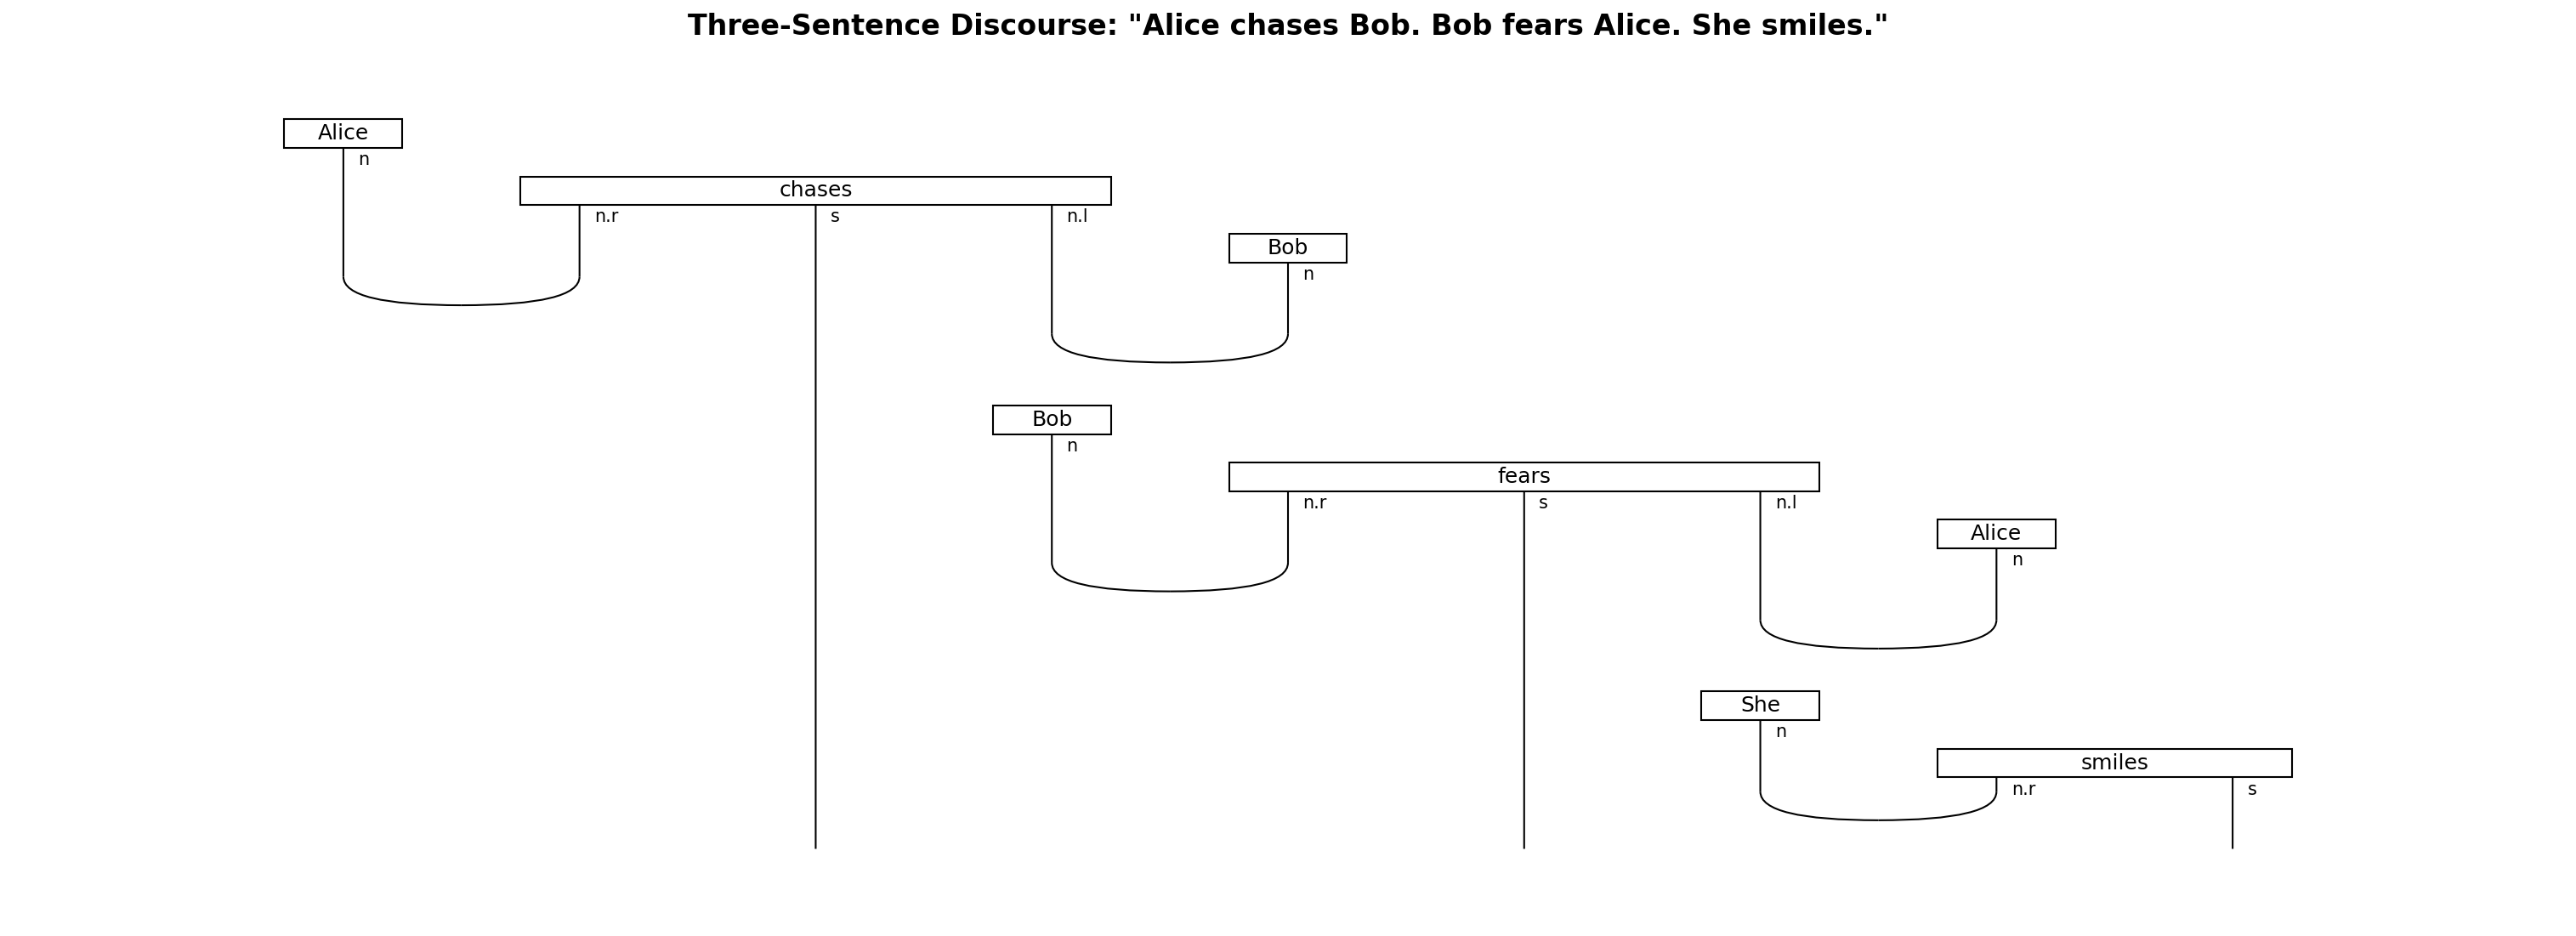
\includegraphics[keepaspectratio,alt={Three-sentence discourse diagram ``Alice chases Bob. Bob fears Alice. She smiles.'' rendered using DisCoPy's pregroup grammar. The diagram demonstrates case role reversal: Alice is NOM (agent) in sentence 1, ACC (patient) in sentence 2, and NOM again via the anaphoric pronoun ``She'' in sentence 3. Each sentence reduces independently to type s via cup contractions, and the full discourse is the triple tensor product s \textbackslash otimes s \textbackslash otimes s. This illustrates how DisCoCirc-style analyses track dynamic case assignment across discourse boundaries.}]{../figures/discopy_three_sentence_discourse.png}}
\caption{Three-sentence discourse diagram ``Alice chases Bob. Bob fears
Alice. She smiles.'' rendered using DisCoPy's pregroup grammar. The
diagram demonstrates case role reversal: Alice is NOM (agent) in
sentence 1, ACC (patient) in sentence 2, and NOM again via the anaphoric
pronoun ``She'' in sentence 3. Each sentence reduces independently to
type s via cup contractions, and the full discourse is the triple tensor
product \(s \otimes s \otimes s\). This illustrates how DisCoCirc-style
analyses track dynamic case assignment across discourse
boundaries.}\label{fig:three-sentence-discourse}
\end{figure}

\subsubsection{Quantum NLP and the lambeq
Pipeline}\label{quantum-nlp-and-the-lambeq-pipeline}

The categorical structure of DisCoCat maps naturally onto quantum
circuits: the tensor product structure of \(\mathbf{FVect}\) is
identical to the tensor product structure of \(\mathbf{Qubit}\), the
category of qubit systems. This observation underlies the \textbf{QNLP}
(Quantum Natural Language Processing) program
\citep{meichanetzidis2020qnlp}, which implements DisCoCat models as
parameterized quantum circuits.

The \textbf{lambeq} library \citep{lorenz2023lambeq} provides a
practical pipeline:

\begin{enumerate}
\def\labelenumi{\arabic{enumi}.}
\tightlist
\item
  Parse a sentence into a pregroup derivation
\item
  Convert the derivation into a string diagram
\item
  Translate the diagram into a parameterized quantum circuit (or a
  classical tensor network)
\item
  Train the parameters on NLP tasks (classification, similarity,
  question answering)
\end{enumerate}

Kartsaklis et al. \citeyearpar{kartsaklis2021functorial} demonstrate
that this pipeline achieves competitive performance on
question-answering tasks, confirming that the categorical structure
captures genuine linguistic regularities even when instantiated on noisy
near-term quantum hardware.

For our case-theoretic framework, QNLP offers a concrete computational
substrate: case categories could be implemented as quantum circuits
where case roles correspond to quantum registers and grammatical
relations correspond to parameterized gates. This connection between
linguistic case structure and quantum information processing---mediated
entirely by the shared categorical formalism---illustrates the power of
the diagrammatic approach.

\newpage

\section{Enriched Category Theory and Distributional Measures of
Language}\label{sec:enriched-categories}

\subsection{Beyond Discrete Categories: Quantitative
Grading}\label{beyond-discrete-categories-quantitative-grading}

The categories introduced in \autoref{sec:case-systems}---with case
roles as objects and grammatical relations as morphisms---capture the
\emph{qualitative} structure of case systems: which roles exist and how
they connect. But linguistic data is fundamentally \emph{quantitative}:
some grammatical relations are more probable than others, some role
assignments are stronger than others, and distributional similarity is a
matter of degree.

To accommodate this quantitative dimension, we move from ordinary
categories to \textbf{enriched categories}, where hom-sets are not just
sets of morphisms but carry additional algebraic structure. The
framework of Bradley et al. \citeyearpar{fritz2021enriched} provides the
key construction.

\subsection{\texorpdfstring{The \([0,1]\)-Enrichment of Case
Categories}{The {[}0,1{]}-Enrichment of Case Categories}}\label{the-01-enrichment-of-case-categories}

\subsubsection{Definition}\label{definition}

A category \(\mathcal{C}\) enriched over the unit interval
\(([0,1], \cdot, 1)\) assigns to every pair of objects \(A, B\) a
\emph{hom-value} \(\mathcal{C}(A, B) \in [0,1]\) satisfying:

\[\mathcal{C}(A, A) = 1 \quad \text{(Identity)} \tag{5.1}\]

\[\mathcal{C}(A, C) \geq \mathcal{C}(A, B) \cdot \mathcal{C}(B, C) \quad \text{(Composition)} \tag{5.2}\]

The identity axiom says that every expression is maximally related to
itself. The composition inequality says that distributional relatedness
composes sub-multiplicatively: if \(A\) is 80\% related to \(B\) and
\(B\) is 70\% related to \(C\), then \(A\) must be at least
\(0.8 \times 0.7 = 56\%\) related to \(C\).

\subsubsection{Interpreting Hom-Values in Linguistic
Context}\label{interpreting-hom-values-in-linguistic-context}

Bradley et al. \citeyearpar{fritz2021enriched} interpret hom-values as
\emph{conditional probabilities} in a distributional model:
\(\mathcal{C}(A, B) = P(\text{context} \mid A \text{ and } B \text{ co-occur})\).
In our case-theoretic application, we interpret them more broadly:

{\def\LTcaptype{none} % do not increment counter
\begin{longtable}[]{@{}
  >{\raggedright\arraybackslash}p{(\linewidth - 4\tabcolsep) * \real{0.3333}}
  >{\raggedright\arraybackslash}p{(\linewidth - 4\tabcolsep) * \real{0.3333}}
  >{\raggedright\arraybackslash}p{(\linewidth - 4\tabcolsep) * \real{0.3333}}@{}}
\toprule\noalign{}
\begin{minipage}[b]{\linewidth}\raggedright
Hom-value interpretation
\end{minipage} & \begin{minipage}[b]{\linewidth}\raggedright
Domain
\end{minipage} & \begin{minipage}[b]{\linewidth}\raggedright
Example
\end{minipage} \\
\midrule\noalign{}
\endhead
\bottomrule\noalign{}
\endlastfoot
Conditional probability & Corpus statistics & P(ACC role \mid{}
transitive verb context) \\
Proto-role strength & Semantic typology & Degree of Proto-Agent
satisfaction \\
Distributional similarity & Vector semantics & Cosine similarity of
case-role embeddings \\
Morphological predictability & Morpholexicology & Reliability of
case-marking paradigm \\
\end{longtable}
}

\subsubsection{Implementation via the EnrichedCategory
Class}\label{implementation-via-the-enrichedcategory-class}

Our \texttt{EnrichedCategory} class implements this structure directly:

\begin{Shaded}
\begin{Highlighting}[]
\NormalTok{cat }\OperatorTok{=}\NormalTok{ EnrichedCategory(name}\OperatorTok{=}\StringTok{"English Case Proximity"}\NormalTok{)}
\NormalTok{cat.add\_object(}\StringTok{"NOM"}\NormalTok{)}
\NormalTok{cat.add\_object(}\StringTok{"ACC"}\NormalTok{)}
\NormalTok{cat.add\_object(}\StringTok{"DAT"}\NormalTok{)}

\NormalTok{cat.set\_hom(}\StringTok{"NOM"}\NormalTok{, }\StringTok{"ACC"}\NormalTok{, }\FloatTok{0.85}\NormalTok{)  }\CommentTok{\# high: agent/patient often co{-}occur}
\NormalTok{cat.set\_hom(}\StringTok{"ACC"}\NormalTok{, }\StringTok{"DAT"}\NormalTok{, }\FloatTok{0.45}\NormalTok{)  }\CommentTok{\# moderate: object/recipient sometimes overlap}
\NormalTok{cat.set\_hom(}\StringTok{"NOM"}\NormalTok{, }\StringTok{"DAT"}\NormalTok{, }\FloatTok{0.30}\NormalTok{)  }\CommentTok{\# low: subject/recipient rarely merge}

\CommentTok{\# Verify composition inequality: 0.30 \textgreater{}= 0.85 * 0.45 = 0.3825?}
\CommentTok{\# This fails! English NOM{-}DAT is too distant relative to the chain.}
\ControlFlowTok{assert} \KeywordTok{not}\NormalTok{ cat.check\_composition\_inequality(}\StringTok{"NOM"}\NormalTok{, }\StringTok{"ACC"}\NormalTok{, }\StringTok{"DAT"}\NormalTok{)}
\end{Highlighting}
\end{Shaded}

The composition inequality violation here is linguistically meaningful:
it tells us that the NOM→ACC→DAT chain overestimates the direct NOM→DAT
relatedness, reflecting the typological fact that subject--recipient
identity (e.g., in benefactive constructions) is more restricted than
the product of agent--patient and patient--recipient proximities.
\autoref{fig:enriched-heatmap} shows the distributional relations
between case roles as a categorical relation graph.

\begin{figure}
\centering
\pandocbounded{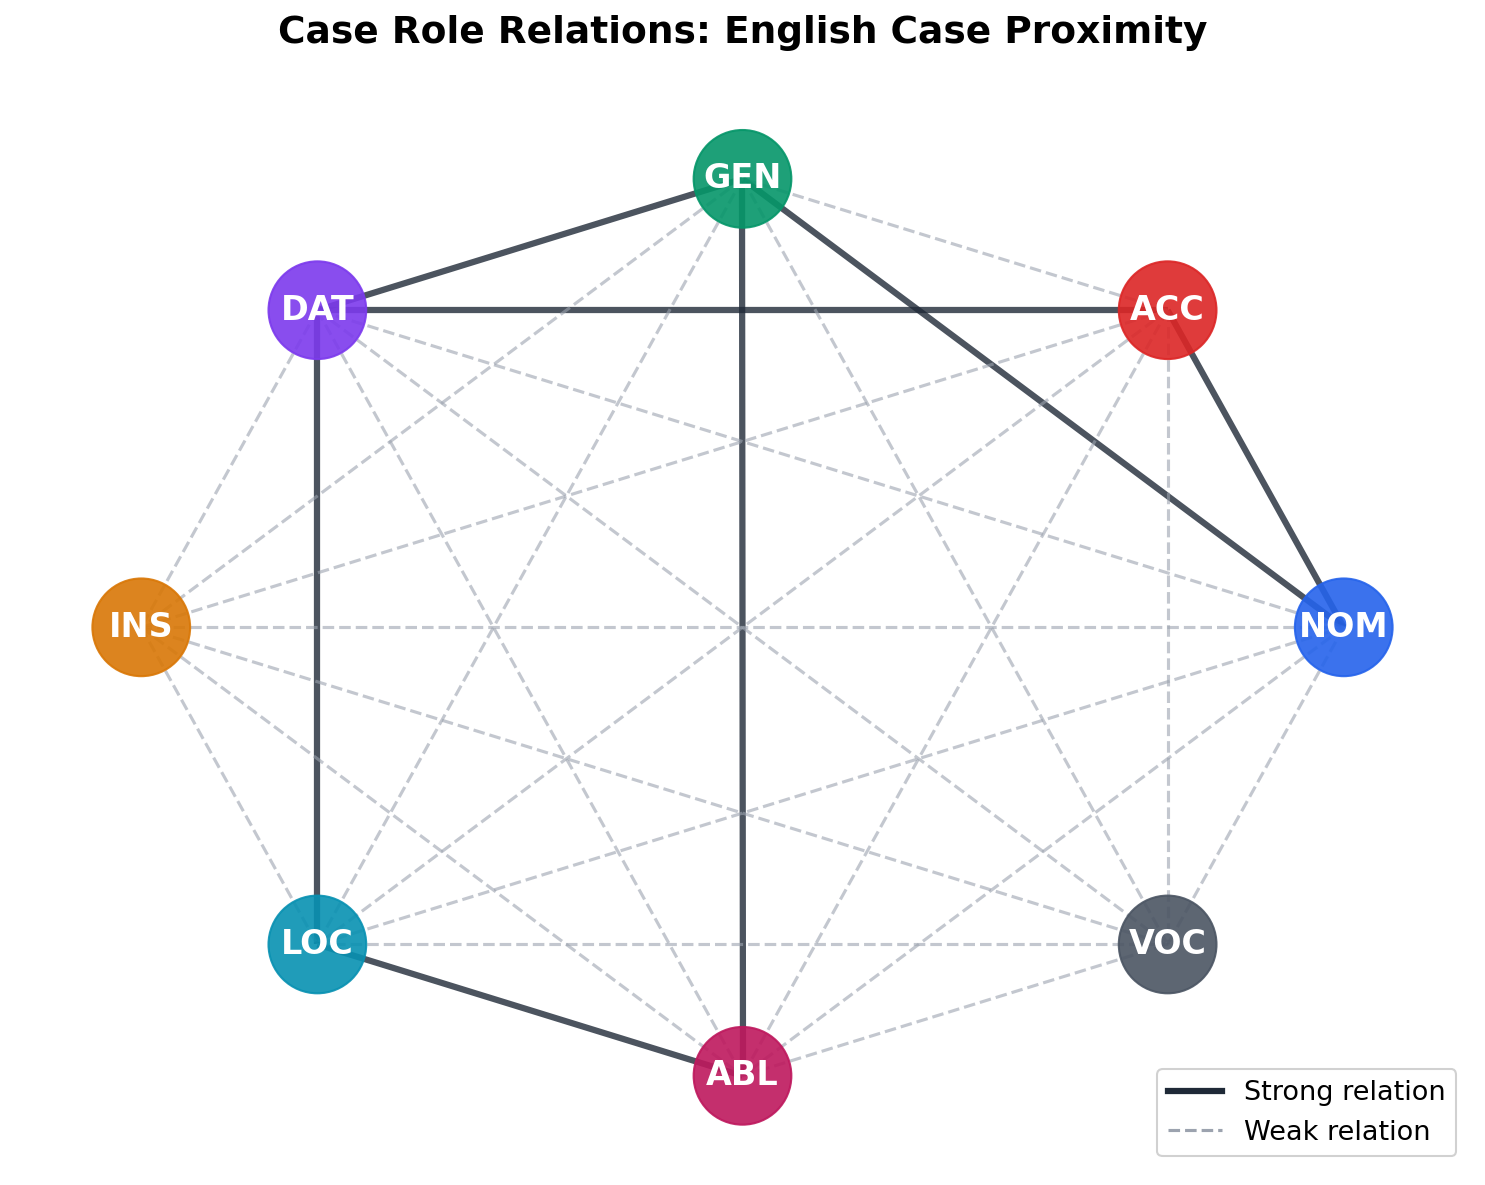
\includegraphics[keepaspectratio,alt={Case role distributional relation graph showing the network of pairwise relationships among all eight case roles (NOM, ACC, GEN, DAT, INS, LOC, ABL, VOC). Strong relations appear as solid edges (indicating frequent co-occurrence or high proto-role overlap), while weaker relations appear as dashed edges. The graph layout reveals clusters of semantically proximate roles (e.g., NOM - ACC, DAT - GEN) and the relative isolation of peripheral cases (VOC, ABL).}]{../figures/enriched_hom_matrix.png}}
\caption{Case role distributional relation graph showing the network of
pairwise relationships among all eight case roles (NOM, ACC, GEN, DAT,
INS, LOC, ABL, VOC). Strong relations appear as solid edges (indicating
frequent co-occurrence or high proto-role overlap), while weaker
relations appear as dashed edges. The graph layout reveals clusters of
semantically proximate roles (e.g., NOM - ACC, DAT - GEN) and the
relative isolation of peripheral cases (VOC,
ABL).}\label{fig:enriched-heatmap}
\end{figure}

\subsection{Categorical Magnitude as a Complexity
Invariant}\label{categorical-magnitude-as-a-complexity-invariant}

A key invariant of enriched categories is their \textbf{magnitude}---a
numerical quantity that captures the ``effective size'' of the category,
discounting for overlap between objects.

For an enriched category with \(n\) objects, let \(Z\) be the
\(n \times n\) matrix with \(Z_{ij} = \mathcal{C}(i, j)\). The magnitude
is:

\[|\mathcal{C}| = \sum_{i,j} (Z^{-1})_{ij} \tag{5.3}\]

when \(Z\) is invertible. Magnitude has deep connections to information
theory:

\begin{itemize}
\tightlist
\item
  For a \emph{discrete} category (no non-trivial relationships),
  \(|\mathcal{C}| = n\) (the number of objects)
\item
  For a highly connected category, \(|\mathcal{C}| < n\) (objects are
  ``redundant'')
\item
  Magnitude connects to the diversity measures studied in ecology
  (species diversity), graph theory (effective graph resistance), and
  information geometry (Fisher information)
\end{itemize}

Bradley \citeyearpar{bradley2020entropy} establishes a foundational link
between categorical magnitude and information entropy through
topological operad derivations. Her result shows that Shannon entropy
can be characterized as the unique derivation of a certain topological
operad---a categorical structure that also governs the composition of
enriched categories. This provides a deep theoretical justification for
using magnitude as a measure of linguistic complexity: the magnitude of
a case category quantifies how much ``information'' the case system
encodes about relational structure.

\subsection{Enriched Functors, Bradley's Language-as-Category Model, and
the LLM
Connection}\label{enriched-functors-bradleys-language-as-category-model-and-the-llm-connection}

Bradley's
\citetext{\citeyear{bradley2024ipam}; \citeyear{bradley2025tea}} broader
program treats natural language itself as an enriched category, where:

\begin{itemize}
\tightlist
\item
  \textbf{Objects} are expressions (words, phrases, sentences)
\item
  \textbf{Hom-values} encode distributional co-occurrence probabilities
\item
  \textbf{Composition} models transitivity of distributional relatedness
\end{itemize}

This ``language as enriched category'' perspective has profound
implications for case theory:

\begin{enumerate}
\def\labelenumi{\arabic{enumi}.}
\item
  \textbf{Case roles emerge from distributional structure}: Rather than
  being imposed a priori, case distinctions arise from clusters of high
  hom-values in the enriched language category. Nouns that frequently
  appear in agent contexts cluster together, forming the ``nominative''
  region of the category.
\item
  \textbf{Alignment types correspond to enriched structure}: Different
  languages partition the enriched category differently, and these
  partitions correspond to the alignment types (accusative, ergative,
  etc.) discussed in \autoref{sec:case-systems}.
\item
  \textbf{Language models are enriched functors}: A neural language
  model (such as a transformer) can be viewed as an enriched functor
  from the syntactic category to the semantic category, mapping
  type-logical derivations to distributional meaning representations
  while preserving the enriched structure.
\end{enumerate}

The deep connection to modern distributional semantics is this: the
static word embeddings of Word2Vec \citep{mikolov2013efficient} and
GloVe \citep{pennington2014glove} operationalize the enriched hom-values
as \emph{cosine similarities} in a learned vector
space---\(\mathcal{C}(A, B) = \cos(\vec{v}_A, \vec{v}_B)\)---while
contextualized embeddings from transformers
\citep{devlin2019bert, vaswani2017attention} compute \emph{dynamic}
hom-values that depend on the sentential context. In the
enriched-categorical framework, this transition from static to
contextualized embeddings corresponds to moving from a \emph{fixed}
enriched category (where hom-values are precomputed from corpus
statistics) to a \emph{parameterized} enriched category (where
hom-values are computed on-the-fly by attention mechanisms). Transformer
attention weights \(\alpha_{ij}\) are precisely such context-dependent
enriched hom-values: they encode how ``related'' token \(i\) is to token
\(j\) in a given representational layer, satisfying a softmax
normalization that parallels the probabilistic interpretation of Bradley
et al.'s \citeyearpar{fritz2021enriched} hom-values as conditional
probabilities.

\subsection{Connection to Lawvere's Metric Spaces and Generalized
Logic}\label{connection-to-lawveres-metric-spaces-and-generalized-logic}

The \([0,1]\)-enrichment connects to a deep tradition in categorical
algebra. Lawvere showed that metric spaces are categories enriched over
\(([0, \infty], +, 0)\): the hom-value is the distance between points,
the identity axiom says \(d(x, x) = 0\), and the composition inequality
is the triangle inequality \(d(x, z) \leq d(x, y) + d(y, z)\). Our
\([0,1]\)-enrichment is the multiplicative analogue: hom-values are
\emph{similarities} rather than distances, and the composition
inequality is sub-multiplicative rather than sub-additive.

This Lawvere-style perspective unifies our case categories with the
geometry of distributional semantics: case roles are points in a
``similarity space,'' and morphisms between them are paths weighted by
distributional proximity. The magnitude of this space then quantifies
the ``effective dimensionality'' of the case system---how many
independent relational distinctions the language makes.

\newpage

\section{Topos-Theoretic Bridges and Inter-Theoretic
Transfer}\label{sec:topos-theory}

\subsection{From Categories to Toposes: The Translation
Problem}\label{from-categories-to-toposes-the-translation-problem}

The preceding sections have shown how case systems, categorial grammars,
distributional semantics, and enriched categories each provide a
different ``window'' onto the same underlying linguistic phenomenon. But
how do we know that results proved in one framework transfer to another?
This is the problem of \emph{inter-theoretic translation}---and it is
precisely the problem that Caramello's
\citeyearpar{caramello2016bridges} topos-theoretic bridge technique was
designed to solve.

\subsection{Classifying Toposes and Morita
Equivalence}\label{classifying-toposes-and-morita-equivalence}

\subsubsection{What Is a Topos? Generalized Universes of
Sets}\label{what-is-a-topos-generalized-universes-of-sets}

A \textbf{topos} is a category that behaves like a generalized universe
of sets: it has products, exponentials, a subobject classifier (playing
the role of a ``truth-value object''), and enough structure to interpret
first-order logic internally. The category \textbf{Set} of ordinary sets
is a topos, but there are many others---presheaf categories, sheaf
categories over topological spaces, and the categories of models of
geometric theories.

\subsubsection{Classifying Toposes of Geometric
Theories}\label{classifying-toposes-of-geometric-theories}

Every \emph{geometric theory} \(\mathbb{T}\) (a theory axiomatized by
sequents involving only finite conjunctions, arbitrary disjunctions, and
existential quantification) has a \textbf{classifying topos}
\(\mathcal{E}_\mathbb{T}\)---a canonical topos whose models correspond
exactly to the geometric functors from \(\mathcal{E}_\mathbb{T}\) to
other toposes. The classifying topos encodes the theory's ``logical
shape'' independently of any particular model.

Caramello's key insight
\citetext{\citeyear{caramello2016bridges}; \citeyear{caramello2021five}}
is that different theories can share the same classifying topos up to
equivalence---an equivalence known as \textbf{Morita equivalence}. When
two theories \(\mathbb{T}_1\) and \(\mathbb{T}_2\) are Morita equivalent
(\(\mathcal{E}_{\mathbb{T}_1} \simeq \mathcal{E}_{\mathbb{T}_2}\)), any
property that can be expressed as an invariant of the classifying topos
transfers automatically between them.

\subsection{Bridge Theorems for the Four Case
Theories}\label{bridge-theorems-for-the-four-case-theories}

\subsubsection{Formalizing Case Theories as Geometric
Theories}\label{formalizing-case-theories-as-geometric-theories}

We formalize each case-theoretic framework as a geometric theory:

\begin{enumerate}
\def\labelenumi{\arabic{enumi}.}
\item
  \textbf{Typological case theory} \(\mathbb{T}_{\text{typ}}\): Objects
  are case roles, morphisms are grammatical relations, axioms specify
  alignment constraints (e.g., ``S = A'' in accusative alignment).
\item
  \textbf{Type-logical case theory} \(\mathbb{T}_{\text{log}}\): Objects
  are syntactic types, morphisms are Lambek calculus derivations, axioms
  specify well-formedness conditions (pregroup contractions).
\item
  \textbf{Distributional case theory} \(\mathbb{T}_{\text{dist}}\):
  Objects are vector spaces, morphisms are linear maps, axioms specify
  the composition law for distributional meaning (DisCoCat).
\item
  \textbf{Enriched case theory} \(\mathbb{T}_{\text{enr}}\): Objects are
  expressions, morphisms carry \([0,1]\)-valued weights, axioms specify
  the identity and composition inequalities.
\end{enumerate}

\subsubsection{The Bridge Theorem: Morita Equivalence
Chain}\label{the-bridge-theorem-morita-equivalence-chain}

The central claim is that these four theories are related by a chain of
Morita equivalences:

\[\mathcal{E}_{\mathbb{T}_{\text{typ}}} \leftarrow \mathcal{E}_{\mathbb{T}_{\text{bridge}}} \rightarrow \mathcal{E}_{\mathbb{T}_{\text{log}}} \leftarrow \mathcal{E}_{\mathbb{T}_{\text{bridge}'}} \rightarrow \mathcal{E}_{\mathbb{T}_{\text{dist}}} \tag{6.1}\]

where the intermediate toposes are constructed by finding geometric
theories that are simultaneously interpretable in both flanking
frameworks. The Morita equivalence ensures that:

\begin{itemize}
\tightlist
\item
  \textbf{Syntactic theorems port to semantics}: A commutativity result
  proved in the type-logical framework automatically yields a
  compositionality result in the distributional framework.
\item
  \textbf{Typological universals constrain distributional models}:
  Alignment types (accusative, ergative) impose structural constraints
  on the vector spaces used in DisCoCat.
\item
  \textbf{Enriched structure enriches all frameworks}: The
  \([0,1]\)-valued weights from the enriched theory can be pulled back
  to give probabilistic interpretations of typological, logical, and
  distributional constructions.
\end{itemize}

\autoref{fig:functor-alignment} visualizes the alignment functor between
the Accusative and Ergative category instantiations, showing how the
same eight case roles are connected by different morphism structures
under different alignment types.

\begin{figure}
\centering
\pandocbounded{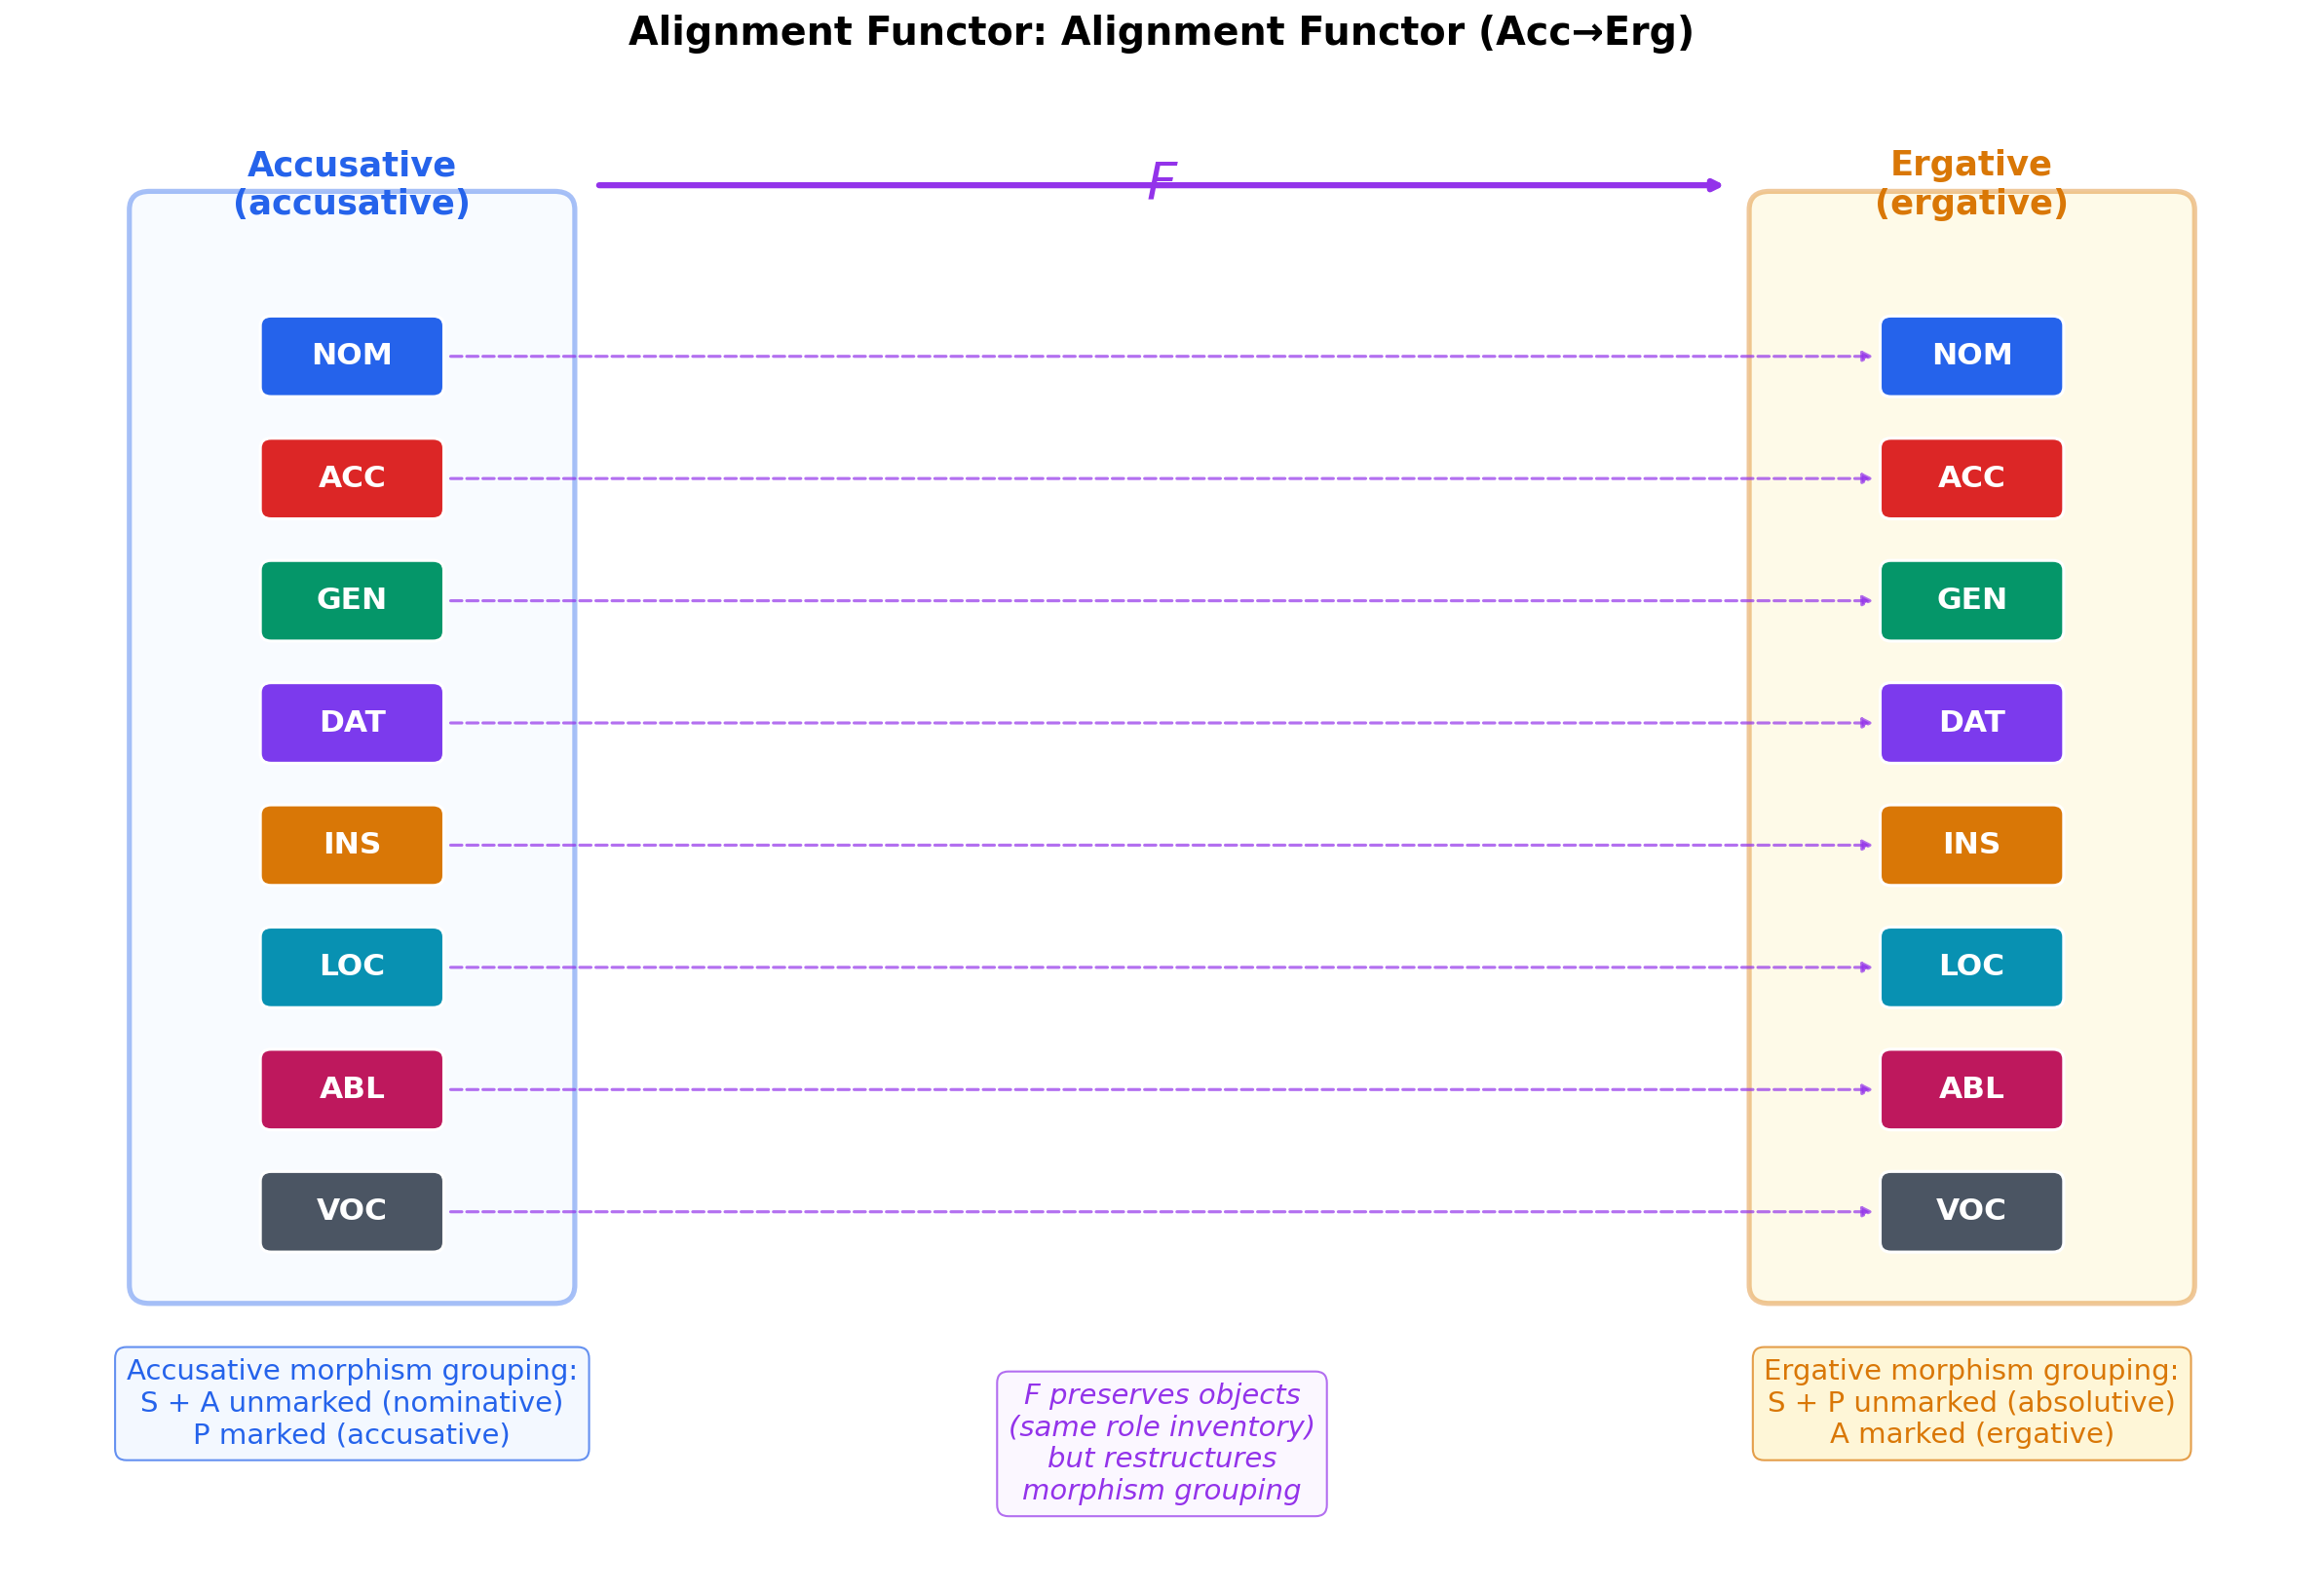
\includegraphics[keepaspectratio,alt={The alignment functor F mapping the Accusative case category (source, blue panel) to the Ergative case category (target, amber panel). Each of the eight case roles (NOM, ACC, GEN, DAT, INS, LOC, ABL, VOC) appears as a labeled node in both categories, with purple horizontal arrows showing the functor's object-level mapping F(role). Below each category, annotations indicate the distinctive morphism grouping: Accusative groups S+A vs.~P (subject and agent unmarked); Ergative groups S+P vs.~A (absolutive unmarked). An explanatory legend clarifies that the functor preserves role inventory but restructures the morphism pattern --- the formal content of the alignment-as-functor principle.}]{../figures/functor_alignment.png}}
\caption{The alignment functor F mapping the Accusative case category
(source, blue panel) to the Ergative case category (target, amber
panel). Each of the eight case roles (NOM, ACC, GEN, DAT, INS, LOC, ABL,
VOC) appears as a labeled node in both categories, with purple
horizontal arrows showing the functor's object-level mapping F(role).
Below each category, annotations indicate the distinctive morphism
grouping: Accusative groups S+A vs.~P (subject and agent unmarked);
Ergative groups S+P vs.~A (absolutive unmarked). An explanatory legend
clarifies that the functor preserves role inventory but restructures the
morphism pattern --- the formal content of the alignment-as-functor
principle.}\label{fig:functor-alignment}
\end{figure}

\subsection{Phillips and the Universal Language of
Thought}\label{phillips-and-the-universal-language-of-thought}

Phillips \citeyearpar{phillips2024lot} provides a striking application
of topos-theoretic methods to cognitive science. He shows that the
\textbf{Language of Thought} (LoT) hypothesis---the claim that cognition
operates over structured, combinatorial representations with
language-like properties---can be formalized categorically, and that the
resulting structure is \emph{universal} in the topos-theoretic sense.

Specifically, Phillips demonstrates that:

\begin{enumerate}
\def\labelenumi{\arabic{enumi}.}
\item
  LoT properties (discrete constituents, role-filler independence,
  systematicity) arise as \textbf{universal constructions} in a
  topos---categorical products, fiber bundles, and presheaves.
\item
  Every topos supports an internal first-order logic, explaining how
  LoT-like logical capacities can emerge in systems (biological or
  artificial) whose internal architecture forms a topos.
\item
  The ``shape'' of cognitive representations is fundamentally
  \textbf{topological}, captured by presheaves and fiber bundles rather
  than by point-set structures.
\end{enumerate}

For our framework, Phillips's result is significant because it provides
a topos-theoretic foundation for the claim that case structure is a
universal feature of cognitive architecture. If the Language of Thought
is topos-universal, and case categories are definable within any topos
(which they are, being small categories with first-order axioms), then
every cognitive system with LoT-like structure must be able to represent
case distinctions---a strong universality claim that goes beyond mere
typological observation.

\subsection{Syntactic Learning via Classifying
Toposes}\label{syntactic-learning-via-classifying-toposes}

Caramello \citeyearpar{caramello2023syntactic} extends the bridge
technique to a learning theory: she shows that classifying toposes can
be used to \emph{learn} the theory of a mathematical structure from
finite data (a finite set of models). The learning algorithm constructs
a classifying topos from the observed data and then extracts the axioms
of the underlying theory.

Applied to case systems, this suggests a principled approach to
\emph{grammatical induction}: given a corpus annotated with case labels,
one could construct the classifying topos of the implicit case theory
and read off its axioms---recovering the alignment type, the morphism
structure, and the enriched weights from data alone. This
topos-theoretic learning procedure would be provably correct (recovering
the true theory in the limit) and maximally general (not presupposing
any particular alignment type).

\subsection{Diagrammatic Implications of Inter-Theoretic
Transfer}\label{diagrammatic-implications-of-inter-theoretic-transfer}

The bridge technique has a natural diagrammatic interpretation. Morita
equivalence between theories is witnessed by \emph{functorial
translations}---diagrams in the 2-category of toposes that commute up to
natural isomorphism. These diagrams serve the same cognitive function as
the commutative diagrams of \autoref{sec:introduction}: they make the
transfer of structure visible, allowing a researcher to verify at a
glance that a result proved in one framework genuinely applies in
another.

Manders \citeyearpar{manders2008euclidean} observed that even in
classical mathematics, diagrams serve not merely as illustrations but as
\emph{inferential instruments} whose spatial properties encode
proof-relevant information. The topos-theoretic bridge diagrams extend
this observation to the meta-theoretical level: the commutative diagram
expressing Morita equivalence is itself a ``free ride'' inference,
automatically transferring any topos-invariant property from one theory
to another without requiring a case-by-case verification.

\newpage

\section{Cognitive Integration: Active Inference, CEREBRUM, and
Diagrammatic Reasoning}\label{sec:cognitive-integration}

\subsection{The Missing Layer: A Dynamic Process Theory of
Cognition}\label{the-missing-layer-a-dynamic-process-theory-of-cognition}

The preceding sections have developed a rich mathematical infrastructure
for analyzing case systems---categorical, type-logical, distributional,
enriched, and topos-theoretic. But these frameworks are \emph{static}:
they describe the structure of case without explaining how a cognitive
agent \emph{uses} that structure in real-time language understanding and
production. What is needed is a \emph{process theory} that explains how
case-marked relational structure is deployed in the dynamic, embodied,
context-sensitive activity of making sense of the world.

Active inference \citep{friston2017active} provides exactly this layer.

\subsection{Active Inference as a Process Theory of Language
Understanding}\label{active-inference-as-a-process-theory-of-language-understanding}

\subsubsection{The Free Energy Principle and Surprise
Minimization}\label{the-free-energy-principle-and-surprise-minimization}

Active inference is the process theory derived from the free energy
principle (FEP): every self-organizing system maintains itself by
minimizing the surprisal (negative log-probability) of its sensory
observations under a \emph{generative model} of its environment
\citeyearpar{friston2010free}. The system does this through two
complementary strategies:

\begin{enumerate}
\def\labelenumi{\arabic{enumi}.}
\tightlist
\item
  \textbf{Perceptual inference}: Update internal beliefs to better
  predict current observations (reduce prediction error)
\item
  \textbf{Active inference}: Act on the environment to bring
  observations in line with predictions (reduce expected prediction
  error)
\end{enumerate}

Recent extensions of active inference to linguistics and cognitive
science have modeled language comprehension and production as forms of
sequential Bayesian inference. As Donnarumma, Frosolone, and Pezzulo
(2023) note in their integration of large language models and active
inference, ``linguistic processing \[is\] inference over a
hierarchical generative model, facilitating predictions and inferences
at various levels of granularity, from syllables to sentences''
\citeyearpar{donnarumma2023integrating}. Similarly, Friston et
al.~(2021) have demonstrated how communication emerges between synthetic
subjects: ``linguistic outcomes (specifically, the spoken word)\ldots{}
are selected to minimise the free energy given current beliefs'' via
``high-order interactions among abstract (discrete) states in deep
(hierarchical) models''
\citetext{\citeyear{friston2021understanding}; \citeyear{friston2020generative}}.

Both strategies minimize the same quantity---variational free
energy---and both are driven by a single generative model that encodes
the system's expectations about the structure of its world.

\subsubsection{Language Understanding as Active Inference over
Relational
Structure}\label{language-understanding-as-active-inference-over-relational-structure}

Language understanding on this view is \emph{active inference over
relational structure}: the listener maintains a generative model of
who-does-what-to-whom, and each incoming word provides evidence that
updates this model. Case marking provides crucial evidence---a
nominative suffix strongly predicts that the marked NP is the agent,
reducing uncertainty about the relational structure of the unfolding
event.

The process unfolds as follows:

\begin{enumerate}
\def\labelenumi{\arabic{enumi}.}
\tightlist
\item
  \textbf{Prior}: The listener has a prior belief about the relational
  structure (a ``case diagram'' encoding expected roles and their
  connections)
\item
  \textbf{Observation}: Each word provides sensory evidence---its form,
  its case marking, its distributional properties
\item
  \textbf{Update}: The listener updates the case diagram to accommodate
  the evidence, using approximate Bayesian inference (typically
  variational message passing)
\item
  \textbf{Prediction}: The updated diagram generates predictions about
  upcoming words (case-marked NPs, verb valency patterns)
\item
  \textbf{Action}: In production, the speaker selects words and case
  markers that minimize expected free energy---choosing expressions that
  are informative, contextually appropriate, and syntactically
  well-formed
\end{enumerate}

\subsubsection{Connection to Barwise and Perry's Situation
Semantics}\label{connection-to-barwise-and-perrys-situation-semantics}

This active inference perspective connects directly to the
\textbf{situation semantics} of Barwise and Perry
\citeyearpar{barwise1983situations}, which conceptualized meaning as
structured \emph{situations}---collections of typed entities,
properties, and relations individuated by spatial and temporal location.
In our framework:

\begin{itemize}
\tightlist
\item
  A \textbf{situation} corresponds to an instantiated case diagram: a
  specific assignment of entities to case roles, with particular
  morphisms activated
\item
  The \textbf{situation type} corresponds to the case category itself:
  the abstract pattern of roles and relations that the situation
  instantiates
\item
  \textbf{Information flow} between situations corresponds to functorial
  mappings between case categories
\end{itemize}

Active inference adds the dynamic component: the agent moves through a
sequence of situations, updating its case diagram in real time and using
the diagram to predict which situation will come next.

\subsection{Distributional Active Inference: Convergence of Two
Distributional
Traditions}\label{distributional-active-inference-convergence-of-two-distributional-traditions}

A remarkable convergence has recently emerged between
\emph{distributional semantics} in linguistics and \emph{distributional
reinforcement learning} in machine learning, mediated by active
inference. Akgül et al. \citeyearpar{akgul2026distributional} introduce
\textbf{Distributional Active Inference (DAIF)}, which integrates active
inference into the distributional RL framework of Bellemare, Dabney, and
Munos \citeyearpar{bellemare2017distributional}. Where classical RL
optimizes \emph{expected} returns (scalar values), distributional RL
models the \emph{full distribution} of returns---a shift from point
estimates to distributional representations that parallels the shift
from symbolic to distributional semantics in linguistics.

The formal architecture of DAIF proceeds through three stages: (1)
reconstructing active inference via variational Bayesian inference on a
controlled Markov process, expressing priors through Pearl's
do-calculus; (2) defining a \emph{push-forward} operation on
representation paths that maps latent-space trajectories to return
distributions; and (3) deriving a temporal-difference quantile-matching
algorithm that implements active inference without requiring explicit
transition dynamics modeling. The resulting ``push-forward RL'' template
achieves active inference's sample-efficiency advantages within a
model-free computational architecture:

\[\mathbb{E}\left[\sum_{t=0}^{\infty} \gamma^t R(x_t, a_t) \mid x_0, a_0\right] = \int_{\mathcal{S}^{\mathbb{N}_+}} R \circ f \, d(\mathbf{S}_{\#} \mathbb{P}_{x_0, a_0}^{P_\pi}) \tag{7.1}\]

where \(\mathbf{S}_{\#}\) denotes the push-forward measure on
representation paths and \(f: \mathcal{S} \to \mathcal{X}\) is the
stochastic decoder.

The terminological collision between ``distributional'' in
distributional semantics and ``distributional'' in distributional RL is
not mere homonymy---it reflects a deep structural parallel. In both
domains, the core move is the same: \textbf{replacing scalar summaries
with full distributional representations.} In linguistics, this means
replacing symbolic word identities with probability distributions over
contexts (Firth's \citeyearpar{firth1957papers} company-keeping
principle). In RL, it means replacing expected-value estimates with full
return distributions. In active inference, it means replacing point
estimates of world states with variational posterior distributions. The
enriched-categorical framework of \autoref{sec:enriched-categories}
provides the unifying abstraction: all three are instances of
\([0,1]\)-enriched categories where hom-values encode distributional
proximity rather than discrete identity.

For case-theoretic reasoning, DAIF suggests a computational architecture
in which case assignment operates distributional-ly at every level: the
agent maintains not a single case diagram but a \emph{distribution over
case diagrams}, weighted by their posterior probability given the
observed linguistic evidence. Each incoming word updates this
distribution via variational message passing, and the agent's production
choices minimize expected free energy across the full distribution of
possible relational structures---not merely the most likely one. This
distributional perspective on case assignment aligns naturally with the
graded proto-role structure of Dowty \citeyearpar{dowty1991thematic}: a
noun phrase is not categorically ``agent'' or ``patient'' but
distributes probability mass across case roles, with the distribution
sharpening as more evidence accumulates.

\subsection{CEREBRUM: The Computational
Architecture}\label{cerebrum-the-computational-architecture}

\subsubsection{Architecture and Design
Principles}\label{architecture-and-design-principles}

The \textbf{CEREBRUM} framework
\citep{friedman2024cerebrum, cerebrum2024github}---Case-Enabled
Reasoning Engine with Bayesian Representations for Unified
Modeling---provides a computational architecture that implements the
categorical case framework within an active inference engine. CEREBRUM
instantiates the view of Vasil et al. \citeyearpar{vasil2020world} that
human communication is itself active inference: a process of jointly
constructing and refining generative models of shared relational
structure.

CEREBRUM's key design principles:

{\def\LTcaptype{none} % do not increment counter
\begin{longtable}[]{@{}
  >{\raggedright\arraybackslash}p{(\linewidth - 2\tabcolsep) * \real{0.5000}}
  >{\raggedright\arraybackslash}p{(\linewidth - 2\tabcolsep) * \real{0.5000}}@{}}
\toprule\noalign{}
\begin{minipage}[b]{\linewidth}\raggedright
Principle
\end{minipage} & \begin{minipage}[b]{\linewidth}\raggedright
Implementation
\end{minipage} \\
\midrule\noalign{}
\endhead
\bottomrule\noalign{}
\endlastfoot
\textbf{Cases as functional roles} & Model components carry case
markings that determine their computational role in the inference
cycle \\
\textbf{Morphisms as message passing} & Grammatical relations are
implemented as message-passing channels between components \\
\textbf{Enriched weights as precision} & The \([0,1]\) weights on
morphisms correspond to precision parameters in the variational
inference scheme \\
\textbf{Alignment as model selection} & Different alignment types
correspond to different generative model architectures, selected by
Bayesian model comparison \\
\textbf{Diagrams as generative models} & Commutative diagrams serve as
the structural specification of the generative model \\
\end{longtable}
}

\subsubsection{Case Roles as Functional Specializations in
CEREBRUM}\label{case-roles-as-functional-specializations-in-cerebrum}

CEREBRUM deploys the eight traditional cases as functional
specializations:

{\def\LTcaptype{none} % do not increment counter
\begin{longtable}[]{@{}lll@{}}
\toprule\noalign{}
Case & CEREBRUM Function & Active Inference Role \\
\midrule\noalign{}
\endhead
\bottomrule\noalign{}
\endlastfoot
NOM & Primary driver / agent & Source of action policies \\
ACC & Primary target / patient & Object of predictions \\
GEN & Source / possessor & Provider of priors \\
DAT & Recipient / goal & Target of information transfer \\
INS & Instrument / means & Tool for state transformation \\
LOC & Context / environment & Markov blanket boundary \\
ABL & Origin / cause & Source of causal influence \\
VOC & Addressee & Pragmatic pointer \\
\end{longtable}
}

\subsection{Diagrammatic Reasoning as a Cognitive Process
Theory}\label{diagrammatic-reasoning-as-a-cognitive-process-theory}

\subsubsection{Diagrams as the Format of Generative
Models}\label{diagrams-as-the-format-of-generative-models}

The claim from \autoref{sec:introduction} can now be strengthened:
commutative diagrams are not merely convenient representations of case
structure---they are the \emph{format} in which cognitive agents
maintain their generative models of relational structure.

This claim is supported by converging evidence:

\begin{enumerate}
\def\labelenumi{\arabic{enumi}.}
\item
  \textbf{Computational advantage} (Larkin \& Simon,
  \citeyearpar{larkin1987diagram}): Diagrams enable search, recognition,
  and inference operations that are computationally prohibitive in
  sentential format. A commutative case diagram allows the agent to
  verify consistency (does the direct path equal the composed path?) by
  simple spatial inspection.
\item
  \textbf{Free ride inferences} (Shimojima,
  \citeyearpar{shimojima1996reasoning}): Properties of the diagram that
  are perceptually available but would require explicit computation in a
  sentential format. In a case diagram, transitivity of grammatical
  relations is \emph{visible}---the existence of a path from NOM to DAT
  through ACC is spatially apparent.
\item
  \textbf{Hybrid reasoning} (Giardino,
  \citeyearpar{giardino2017diagrammatic}): Mathematical diagrams engage
  a mode of reasoning that combines perceptual pattern recognition with
  background theoretical knowledge. Case diagrams similarly engage both
  the perceptual system (spatial layout) and linguistic knowledge (case
  constraints, verb valency).
\item
  \textbf{Peirce's existential graphs}: Peirce's graphical logic system
  demonstrated that first-order logic can be conducted entirely
  diagrammatically, without algebraic symbols. Our case diagrams extend
  this tradition: the relational structure of a sentence is represented
  graphically, and inference proceeds by diagram manipulation
  (adding/removing nodes, composing morphisms).
\end{enumerate}

\subsubsection{Predictive Processing and Diagrammatic Belief
Updating}\label{predictive-processing-and-diagrammatic-belief-updating}

The predictive processing framework---of which active inference is the
most developed version---provides a natural account of how diagrammatic
representations are used cognitively:

\begin{enumerate}
\def\labelenumi{\arabic{enumi}.}
\item
  \textbf{Top-down predictions}: The current case diagram generates
  predictions about expected sensory input (e.g., ``a nominative-marked
  NP should appear because the transitive verb requires an agent'')
\item
  \textbf{Bottom-up prediction errors}: Incoming words that violate the
  diagrammatic predictions generate prediction errors (e.g., an
  unexpected case marker triggers a P600 event-related potential in the
  brain)
\item
  \textbf{Belief updating}: The diagram is updated to accommodate the
  prediction error, potentially restructuring the assignment of entities
  to case roles (garden-path reanalysis)
\item
  \textbf{Precision weighting}: The enriched weights on morphisms serve
  as \emph{precision parameters} that control the relative influence of
  prior expectations and incoming evidence. A high-weight morphism
  generates strong predictions that are costly to override; a low-weight
  morphism generates weak predictions that are easily overridden.
\end{enumerate}

\subsection{Total Cognitive Scenario Understanding: The Integrated
Framework}\label{total-cognitive-scenario-understanding-the-integrated-framework}

The full picture emerges when we combine all five pillars within the
active inference framework:

\begin{enumerate}
\def\labelenumi{\arabic{enumi}.}
\tightlist
\item
  \textbf{Case categories} (\autoref{sec:case-systems}) provide the
  \emph{objects and morphisms} of the generative model---the vocabulary
  of roles and relations
\item
  \textbf{Categorial grammar} (\autoref{sec:categorial-grammar})
  provides the \emph{composition rules}---how roles combine to form
  structured derivations
\item
  \textbf{DisCoCat/DisCoCirc} (\autoref{sec:categorical-semantics})
  provides the \emph{semantic functor}---mapping syntactic structure to
  distributional meaning
\item
  \textbf{Enriched structure} (\autoref{sec:enriched-categories})
  provides the \emph{precision parameters}---graded weights that control
  inference
\item
  \textbf{Topos-theoretic bridges} (\autoref{sec:topos-theory}) provide
  \emph{transfer theorems}---ensuring consistency across formalizations
\end{enumerate}

The active inference agent uses this combined structure as a single,
integrated generative model. Each scenario it encounters---a sentence
heard, a scene observed, an action planned---is interpreted by
instantiating a case diagram from structure (1), parsing the input using
rules (2), computing meaning via the semantic functor (3), weighting
confidence using enriched structure (4), and transferring results across
representational formats using bridge techniques (5).

This is \emph{total cognitive scenario understanding}: the agent doesn't
just parse a sentence or assign case labels---it constructs a complete,
internally consistent, generic, strongly typed, dynamically updating
model of the relational structure of the situation, and uses that model
to predict, explain, and act.

\subsection{Computational Verification and Test
Suite}\label{computational-verification-and-test-suite}

The framework developed in this paper is not merely theoretical---it is
computationally verified through a comprehensive implementation and test
suite that exercises every categorical construction discussed above.

\subsubsection{Implementation Architecture and Categorical
Core}\label{implementation-architecture-and-categorical-core}

The categorical core (\texttt{CaseCategory}, \texttt{EnrichedCategory},
\texttt{CaseFunctor}, \texttt{NaturalTransformation}) is implemented in
Python with networkx-backed directed graphs, enforcing categorical
axioms at construction time. The visualization layer produces all 15
manuscript figures programmatically, ensuring exact correspondence
between formal claims and visual evidence. The DisCoPy integration
library (version 1.2.2) provides an independent validation path:
pregroup types (\texttt{Ty}), lexical entries (\texttt{Word}), cup
contractions (\texttt{Cup}), cap expansions (\texttt{Cap}), type
permutations (\texttt{Swap}), normal form computation
(\texttt{normal\_form()}), and circuit depth analysis (\texttt{depth()})
are exercised against the same categorical structures described in
\autoref{sec:categorial-grammar} and
\autoref{sec:categorical-semantics}.

\subsubsection{Test Suite and Coverage
Metrics}\label{test-suite-and-coverage-metrics}

The implementation is validated by \textbf{158 automated tests} across 8
test files with \textbf{95.97\% code coverage} (against a 90\% threshold
enforced in the build configuration). Every test uses real mathematical
computations---no mocks or fakes:

\begin{itemize}
\tightlist
\item
  \textbf{Categorical axiom tests}: Identity morphism existence,
  composition associativity, weight invariants
\item
  \textbf{Enriched category tests}: Hom-value constraints, composition
  inequality, categorical magnitude
\item
  \textbf{Diagram type tests}: Pregroup diagrams validated for
  \texttt{dom\ ==\ Ty()} and \texttt{cod\ ==\ s}, correct box counts,
  diagram equality
\item
  \textbf{Metrics tests}: Normal form preservation, depth computation
  with graceful fallback for pregroup diagrams
\end{itemize}

This computational verification demonstrates that the category-theoretic
framework is not just a mathematical convenience but a \emph{working
computational architecture}---the categorical abstractions compile,
execute, and produce verifiable results, bridging the gap between formal
theory and implemented system.

\newpage

\section{Quantum Active Inference: Topological Diagrams as Semantic
Computation}\label{sec:quantum-active-inference}

The preceding sections have established that categorical string
diagrams---from DisCoCat's pregroup derivations
(\autoref{sec:categorical-semantics}) through enriched hom-values
(\autoref{sec:enriched-categories}) to topos-theoretic transfer
(\autoref{sec:topos-theory})---provide a unified diagrammatic language
for case-theoretic reasoning. This section extends the framework into
its natural quantum generalization: topological quantum neural networks
(TQNNs), the ZX-calculus, and sheaf-theoretic quantum semantic
communication. The central observation is that the same
monoidal-categorical architecture that underlies DisCoCat string
diagrams also underlies quantum circuits, TQFT cobordisms, and quantum
information flow---making active inference on case-marked relational
structure a quantum topological computation.

\subsection{Topological Quantum Neural Networks and Spin-Network
Representations}\label{topological-quantum-neural-networks-and-spin-network-representations}

\subsubsection{From Quantum Neural Networks to
TQFT}\label{from-quantum-neural-networks-to-tqft}

Marcianò, Fields, and Glazebrook demonstrate that quantum neural
networks (QNNs) admit a topological reformulation via spin-networks
\citep{fields2022tqnn}. In their analysis, a QNN layer or connectivity
pattern is represented as a graph whose edges carry representation
labels (spins) and whose vertices carry intertwiners---precisely the
graphical data of a spin-network in a 3-dimensional topological quantum
field theory:

\begin{quote}
``Quantum Neural Networks (QNNs) can be mapped onto spin-networks, with
the consequence that the level of analysis of their operation can be
carried out on the side of Topological Quantum Field Theory (TQFT).''
\citep{fields2022tqnn}
\end{quote}

This reformulation has three important structural consequences. First,
the neural architecture becomes a topological diagram (spin-network /
ribbon graph) whose evaluation by a TQFT functor gives a quantum
process; the edges and nodes of the graph encode how quantum information
flows and transforms. Second, the TQFT evaluation functorially assigns
to boundary Hilbert spaces (inputs/outputs) linear maps obtained from
topological invariants (Reshetikhin--Turaev, Turaev--Viro), playing the
role of the network's forward pass: amplitudes ``flow'' through the
topological diagram. Third, the topological control structure encodes
information flow through the network's wiring topology rather than
through any fixed geometric embedding \citep{fields2023tensor}.

\subsubsection{Universal Quantum Computation via
TQNNs}\label{universal-quantum-computation-via-tqnns}

Fields and collaborators further demonstrate that TQNNs are universal
quantum computers by identifying the Reshetikhin--Turaev invariant of a
TQNN with a Turaev--Viro quantum error-correcting code:

\begin{quote}
``TQNNs enable universal quantum computation, using the
Reshetikhin-Turaev and Turaev-Viro models to show how TQNNs implement
quantum error-correcting codes.'' \citep{fields2025amplituhedra}
\end{quote}

The universality result is established via the concept of an
\emph{execution trace} for a quantum computation, leading to the
representation of TQNNs in terms of the positive geometries provided by
amplituhedra---a deep connection between quantum computation, scattering
amplitudes, and topological combinatorics.

\subsubsection{Quantum Reference Frames and Holographic
Screens}\label{quantum-reference-frames-and-holographic-screens}

Fields and Glazebrook's work on quantum reference frames (QRFs) and
holographic screens provides additional algebraic structure
\citep{fields2021qrf}. A holographic screen---the information boundary
between two interacting quantum systems---carries a qubit array encoding
their interaction. The key insight is that QRFs deployed to identify
systems and select pointer states induce decoherence, breaking the
symmetry of the holographic encoding in an observer-relative way. This
symmetry-breaking is precisely the mechanism by which a TQNN
``observes'' its input: the choice of QRF determines the basis in which
the spin-network is evaluated.

For case-theoretic reasoning, this connects to the grammatical observer
problem: a parser or comprehender selecting a case-assignment frame for
a sentence is analogous to deploying a QRF that fixes the pointer basis
for a quantum measurement on a holographic screen.

\subsection{The ZX-Calculus: Categorical Quantum Circuit
Diagrams}\label{the-zx-calculus-categorical-quantum-circuit-diagrams}

\subsubsection{String Diagrams for Quantum
Processes}\label{string-diagrams-for-quantum-processes}

The ZX-calculus provides a categorical, diagrammatic language in which
quantum circuits are drawn as string diagrams in a symmetric monoidal
category of finite-dimensional Hilbert spaces and linear maps
\citep{kissinger2020zx}:

\begin{quote}
``The ZX-calculus is a graphical language for reasoning about quantum
computations and circuits\ldots{} it can represent any linear map, and
can be considered a diagrammatically complete generalization of the
usual circuit representation.'' \citep{coeckekissinger2017}
\end{quote}

Several structural features are critical for the connection to
case-theoretic diagrams:

\begin{itemize}
\tightlist
\item
  \textbf{Diagrams as morphisms}: ZX-diagrams are string diagrams in a
  \(\dagger\)-compact closed category. Wires represent objects (qubits),
  spiders and boxes represent morphisms, and composition/tensor product
  correspond to vertical/horizontal gluing. No metric geometry
  enters---only the topology of connections. ZX is therefore already a
  \emph{topological} representation of quantum processes.
\item
  \textbf{Circuit extraction via generalized flow}: Kissinger and van de
  Wetering demonstrate that quantum circuits can be mapped into
  ZX-diagrams, subjected to purely graph-theoretic (topological)
  transformations, and then extracted as optimized circuits. They prove
  that ``the underlying graph of our simplified ZX-diagram always has a
  graph-theoretic property called generalised flow, which in turn yields
  a deterministic circuit extraction procedure''
  \citep{kissinger2020zx}.
\item
  \textbf{Category-theoretic semantics}: The semantics of a ZX-diagram
  are determined entirely by how components are wired
  together---precisely the compositional principle underlying DisCoCat
  and the case categories of \autoref{sec:case-systems}.
\end{itemize}

\subsubsection{From DisCoCat to ZX: A Shared Categorical
Architecture}\label{from-discocat-to-zx-a-shared-categorical-architecture}

The structural parallel between pregroup grammar diagrams and
ZX-diagrams is not accidental. Both are instances of the same
mathematical object: morphisms in a compact closed monoidal category
with functorial semantics into Hilbert spaces. In DisCoCat, the functor
assigns to each grammatical type a vector space and to each derivation a
linear map computing sentence meaning \citep{coecke2010mathematical}. In
ZX, the standard semantics functor assigns to each spider/Hadamard
configuration a linear map in \textbf{FHilb}. The shared categorical
architecture means:

\begin{enumerate}
\def\labelenumi{\arabic{enumi}.}
\tightlist
\item
  \textbf{Pregroup contractions (cups) and ZX spiders} are both
  instances of the same algebraic operation: evaluation morphisms in a
  compact closed category.
\item
  \textbf{DisCoCat normal forms} and \textbf{ZX simplifications} are
  both applications of the same rewriting theory: equational reasoning
  modulo the axioms of a compact closed category.
\item
  \textbf{The snake equation} (Cap \(\circ\) Cup = identity) that
  grounds all pregroup type reductions
  (\autoref{sec:categorical-semantics}) is a special case of the spider
  fusion rule in ZX.
\end{enumerate}

This means that case-theoretic DisCoCat derivations can, in principle,
be compiled into ZX circuits and executed on quantum hardware---a
connection already exploited by the lambeq quantum NLP pipeline
\citep{lorenz2023lambeq}.

\subsection{Aligning TQNNs with Categorical Distributional
Semantics}\label{aligning-tqnns-with-categorical-distributional-semantics}

\subsubsection{Common Language: Ribbon and Tensor
Diagrams}\label{common-language-ribbon-and-tensor-diagrams}

Both ZX-diagrams and TQNNs are topological string diagrams evaluated by
monoidal functors into the category of Hilbert spaces and linear maps.
The alignment becomes explicit when stated precisely:

\begin{itemize}
\tightlist
\item
  \textbf{For TQNNs}: A 3-dimensional TQFT functor from a cobordism or
  skein category to \textbf{Hilb} assigns to each spin-network/ribbon
  graph a linear map representing the TQNN computation. The underlying
  topological skein theory treats network layers as \emph{ribbon graphs}
  whose evaluation via Reshetikhin--Turaev and Turaev--Viro invariants
  gives quantum processes implementing computation and error correction
  \citep{fields2022tqnn, fields2025amplituhedra}.
\item
  \textbf{For ZX}: The standard semantics functor from the free
  \(\dagger\)-compact category generated by Z/X spiders, Hadamards, etc.
  into \textbf{FHilb} assigns each ZX-diagram a linear map
  \citep{kissinger2020zx}.
\item
  \textbf{For DisCoCat}: The meaning functor from the pregroup grammar
  category to \textbf{FdVect} assigns to each grammatical derivation a
  multilinear map computing compositional meaning
  \citep{coecke2010mathematical}.
\end{itemize}

Up to choice of labels and normalization, all three are graphical
calculi for monoidal categories whose morphisms are quantum (or
quantum-like) processes. A layer of a topological quantum flow network
can be modeled as a ZX-diagram fragment whose input and output boundary
wires are the ``feature spaces'' (Hilbert spaces) at successive
processing steps, while internal spiders encode unitary/non-unitary
channels that realize synaptic transformations.

\subsubsection{Neural Flow as Generalized
Flow}\label{neural-flow-as-generalized-flow}

The \emph{generalized flow} condition used to guarantee deterministic
circuit extraction from ZX-diagrams is a graph-theoretic constraint that
ensures a well-defined causal ordering of operations
\citep{kissinger2020zx}. This mirrors the requirement in TQNNs that the
diagram encode a consistent \emph{execution trace} of a quantum
computation. Fields and colleagues make this connection explicit in
their TQNN--amplituhedron correspondence:

\begin{quote}
``\ldots this formal correspondence is stated by Theorem 2 whose proof
draws upon the concept of execution trace for a quantum
computation\ldots{} and thus leads to representing a TQNN in terms of
the positive geometries as provided by amplituhedra.''
\citep{fields2025amplituhedra}
\end{quote}

A topological quantum flow neural network can therefore be regarded as a
ZX-style circuit where the graphical calculus is enriched to a 3D TQFT
skein theory, but the \emph{abstract type} of object---a topological
string diagram with functorial semantics---remains the same.

\subsection{Distributional Semantics on Topological Quantum
Flow}\label{distributional-semantics-on-topological-quantum-flow}

\subsubsection{Meaning Spaces as Hilbert
Spaces}\label{meaning-spaces-as-hilbert-spaces}

To connect TQNNs and ZX circuits to \emph{distributional semantics}, one
reinterprets the amplitudes and correlations in these diagrams as
semantic quantities. Recent work on quantum semantic communication
provides the theoretical bridge, modeling ``meaning spaces'' as Hilbert
spaces at nodes of a graph with channels as completely positive
trace-preserving (CPTP) maps along edges \citep{khatri2025quantum}:

\begin{quote}
``Multi-agent semantic networks are modeled as quantum sheaves, where
agents' meaning spaces are Hilbert spaces connected by quantum
channels.'' \citep{khatri2025quantum}
\end{quote}

A \emph{quantum semantic sheaf} over a communication graph \(G=(V,E)\)
is defined as a triple \((H,F,\rho)\) where each vertex \(v\) carries a
finite-dimensional Hilbert space \(H_v\), edges carry CPTP maps \(F_e\),
and each vertex has a local density operator \(\rho_v\) encoding its
``current semantic state.'' This is precisely a distributional-semantics
picture: meanings are modeled as vectors/density operators in
high-dimensional spaces, with co-occurrence and context encoded in how
these spaces are functorially related across the network.

\subsubsection{Grafting Distributional Semantics onto the TQNN/ZX
Architecture}\label{grafting-distributional-semantics-onto-the-tqnnzx-architecture}

When this sheaf-theoretic semantics is grafted onto the TQNN/ZX
architecture, three structural correspondences emerge:

\begin{enumerate}
\def\labelenumi{\arabic{enumi}.}
\item
  \textbf{Edges as semantic feature channels}: In a TQNN or ZX-diagram,
  each wire carries not merely an abstract qubit but a semantic Hilbert
  space \(H_v\) associated with a context, concept, or agent. Amplitudes
  or density matrices on that wire encode a distribution over semantic
  features---exactly as word vectors encode distributional meaning in
  classical compositional distributional semantics.
\item
  \textbf{Nodes as compositional operations}: Spiders/gates in ZX or
  intertwiners in TQNNs become \emph{semantic composition maps}: they
  take distributed meanings on input wires and produce new distributed
  meanings on output wires, analogous to how DisCoCat composes word
  meanings into phrase/sentence meanings via multilinear maps.
\item
  \textbf{Topological wiring as contextual structure}: The topology of
  the diagram---the way wires and nodes are connected---encodes which
  semantic spaces interact and in what causal/structural pattern. This
  is the semantic analogue of syntactic structure in distributional
  semantics, realized as a topological quantum circuit.
\end{enumerate}

In this reading, a topological quantum flow neural network becomes a
\emph{distributional semantic machine}: a functor that sends a
topological diagram (graph of contexts and interactions) to a family of
Hilbert spaces and maps where vectors/densities represent distributed
meanings and their probabilistic transformations.

\subsection{Semantic Probabilistic Information Transfer as Functorial
Flow}\label{semantic-probabilistic-information-transfer-as-functorial-flow}

\subsubsection{Sheaf Cohomology and Semantic
Alignment}\label{sheaf-cohomology-and-semantic-alignment}

The sheaf-based framework proves that semantic alignment between agents
is governed by cohomology classes of the quantum semantic sheaf;
contextuality and entanglement act as resources that remove obstructions
to alignment \citep{khatri2025quantum}:

\begin{quote}
``We derive semantic channel capacity when sender and receiver share
prior entanglement, proving it strictly exceeds classical capacity. The
quantum advantage grows as channel noise increases---precisely when
semantic communication most benefits over bit-level transmission.''
\citep{khatri2025quantum}
\end{quote}

Two further results from this framework are particularly relevant:

\begin{itemize}
\tightlist
\item
  \textbf{Contextuality as a semantic resource}: ``Quantum contextuality
  reduces cohomological obstructions to semantic alignment. Contextual
  correlations act as `pre-shared semantic resolution,' establishing
  contextuality as a resource for semantic communication''
  \citep{khatri2025quantum}.
\item
  \textbf{Discord as integrated semantic information}: ``Quantum discord
  equals integrated semantic information, linking quantum correlations
  to irreducible semantic content and connecting our framework to
  integrated information theory'' \citep{khatri2025quantum}.
\end{itemize}

These results establish that the topology of the semantic sheaf (and its
cohomology) constrains how probabilistic semantic information can be
transferred; quantum features (entanglement, contextuality, discord)
change these constraints in well-defined ways.

\subsubsection{Topological Circuit as Semantic Sheaf
Skeleton}\label{topological-circuit-as-semantic-sheaf-skeleton}

A TQNN/ZX circuit implementing a quantum communication or computation
protocol is itself a diagram over which one can define a sheaf of
semantic spaces and channels. The underlying graph of the TQNN/ZX
diagram serves as the base graph \(G=(V,E)\) of the semantic sheaf:
vertices inherit meaning spaces \(H_v\), edges inherit CPTP maps
\(F_e\), and the TQFT/ZX functor gives the global linear map
representing the protocol. Distributional semantics as diagram
evaluation then becomes literal: passing an initial semantic state
(distribution over meanings) through the TQNN/ZX diagram yields an
output state whose components encode the posterior semantic
distributions at boundary wires.

ZX rewrite rules, which change the internal topology of the diagram
while preserving its overall semantics as a linear map, correspond to
alternative factorizations of the same semantic
transformation---different internal ``flow architectures'' for realizing
the same semantic map.

\subsection{Implications for Active Inference and Case
Assignment}\label{implications-for-active-inference-and-case-assignment}

\subsubsection{Case Assignment as Quantum
Measurement}\label{case-assignment-as-quantum-measurement}

The active inference model of case reasoning
(\autoref{sec:cognitive-integration}) acquires a new dimension in this
quantum topological setting. Case assignment---the cognitive process of
determining \emph{who does what to whom}---can be modeled as a quantum
measurement process on a holographic screen, with the following
correspondences:

{\def\LTcaptype{none} % do not increment counter
\begin{longtable}[]{@{}
  >{\raggedright\arraybackslash}p{(\linewidth - 2\tabcolsep) * \real{0.5000}}
  >{\raggedright\arraybackslash}p{(\linewidth - 2\tabcolsep) * \real{0.5000}}@{}}
\toprule\noalign{}
\begin{minipage}[b]{\linewidth}\raggedright
Classical Case Assignment
\end{minipage} & \begin{minipage}[b]{\linewidth}\raggedright
Quantum Topological Model
\end{minipage} \\
\midrule\noalign{}
\endhead
\bottomrule\noalign{}
\endlastfoot
Case role (NOM, ACC, \ldots) & Pointer state selected by QRF \\
Case frame (alignment system) & Quantum reference frame \\
Relational structure of event & Spin-network topology \\
Free-energy minimization & TQFT evaluation of diagram \\
Prediction-error (P600/N400) & Symmetry-breaking on holographic
screen \\
\end{longtable}
}

\subsubsection{From Predictive Processing to Topological
Flow}\label{from-predictive-processing-to-topological-flow}

In the predictive processing account, a cognitive agent maintains a
generative model that predicts the relational structure of incoming
linguistic material. When this model is realized as a TQNN, prediction
becomes evaluation of the topological diagram; prediction error becomes
the discrepancy between the predicted TQFT evaluation and the observed
data; and belief updating becomes modification of the spin-network's
edge labels (representation labels) and vertex intertwiners.

The topological character of this computation confers significant
advantages for active inference on case structure: topological
invariants are robust to continuous deformation, so the generative
model's predictions are stable under small perturbations of the
input---a desirable property for language understanding in noisy
environments.

\subsubsection{Quantum Advantage in Semantic
Communication}\label{quantum-advantage-in-semantic-communication}

The sheaf-theoretic results of Khatri et al.
\citeyearpar{khatri2025quantum} suggest that quantum features provide
genuine advantages for semantic communication---not merely computational
speedup, but qualitative enhancements in semantic alignment. If
case-marked relational structure is communicated between agents via
quantum channels, entanglement provides additional semantic capacity,
contextuality removes alignment obstructions, and discord captures
irreducible semantic content. These are not abstract possibilities but
operational consequences of the mathematical framework developed across
this review. Recent work by Sherborne et al.
\citeyearpar{sherborne2025paramqnlp} demonstrates this concretely:
DisCoCirc string diagrams that represent discourse-level semantics
(including case role assignments across sentences) can be
\emph{automatically} compiled into parameterized quantum circuits,
closing the loop from linguistic case structure through categorical
formalism to quantum computation.

\newpage

\section{Synthetic and Artificial Intelligence: Categorical
Foundations}\label{sec:ai-implications}

\subsection{Compositional Structure in Multi-Agent AI
Communication}\label{compositional-structure-in-multi-agent-ai-communication}

The categorical framework developed in the preceding sections---case
categories, functorial semantics, enriched structure, and diagrammatic
reasoning---addresses a core challenge in contemporary artificial
intelligence: how to endow autonomous agents with structured,
compositional communication.

Current multi-agent AI systems communicate through increasingly
standardized protocols. Google's Agent-to-Agent (A2A) protocol
\citep{google2025a2a}, introduced in 2025, provides a standard way for
agents to communicate regardless of underlying framework through
HTTP/JSON-RPC message passing with capability discovery. The Model
Context Protocol (MCP) \citep{anthropic2024mcp} standardizes how AI
agents access external tools and data sources. The Agent Communication
Protocol (ACP) \citep{acp2025protocol} handles standardizing messaging
formats across various users, including agents, applications, and
humans. The Agent Network Protocol (ANP) \citep{anp2025protocol}
introduces a three-layer architecture supporting trusted agent
interaction in distributed systems. These engineering advances solve
critical interoperability problems but lack a compositional semantics:
messages are flat JSON payloads without inherent algebraic structure.

Category theory provides exactly the missing layer. Just as the DisCoCat
framework maps grammatical derivations functorially into vector spaces
(see \autoref{sec:categorical-semantics}), a categorical communication
protocol would map agent interaction patterns functorially into
behavioral specifications. The morphisms of such a protocol category
would be message types, the objects would be agent states, and the
composition law would specify how multi-step interactions chain
together---exactly the structure of our case categories, where morphisms
represent grammatical relations and composition encodes transitivity.

\subsection{Case Roles as Functional Typing for Agent
Systems}\label{case-roles-as-functional-typing-for-agent-systems}

The eight-case framework of CEREBRUM \citep{friedman2024cerebrum} maps
directly onto the functional roles that components play in multi-agent
architectures:

{\def\LTcaptype{none} % do not increment counter
\begin{longtable}[]{@{}
  >{\raggedright\arraybackslash}p{(\linewidth - 4\tabcolsep) * \real{0.3333}}
  >{\raggedright\arraybackslash}p{(\linewidth - 4\tabcolsep) * \real{0.3333}}
  >{\raggedright\arraybackslash}p{(\linewidth - 4\tabcolsep) * \real{0.3333}}@{}}
\toprule\noalign{}
\begin{minipage}[b]{\linewidth}\raggedright
Case Role
\end{minipage} & \begin{minipage}[b]{\linewidth}\raggedright
Agent System Analogue
\end{minipage} & \begin{minipage}[b]{\linewidth}\raggedright
Protocol Function
\end{minipage} \\
\midrule\noalign{}
\endhead
\bottomrule\noalign{}
\endlastfoot
NOM (Agent) & Active requester & Initiator of action policies \\
ACC (Patient) & Passive responder & Target of directed operations \\
GEN (Source) & Context provider & Supplier of prior information \\
DAT (Recipient) & Designated receiver & Endpoint for information
transfer \\
INS (Instrument) & Tool / API & Means of state transformation \\
LOC (Context) & Environment state & Boundary conditions and Markov
blanket \\
ABL (Origin) & Data source & Causal provenance of inputs \\
VOC (Addressee) & Routing target & Pragmatic addressing in broadcast
networks \\
\end{longtable}
}

This mapping is not merely analogical. In the MCP protocol, a tool call
has precisely the structure of a case-marked clause: an \emph{agent}
(NOM) invokes a \emph{tool} (INS) on a \emph{resource} (ACC) to deliver
a \emph{result} to a \emph{recipient} (DAT). The case structure ensures
that every interaction is relationally typed, preventing the category
errors (sending a response where a tool call is expected) that plague
unstructured message-passing systems.

\subsection{Categorical Deep Learning: An Algebraic Theory of
Architectures}\label{categorical-deep-learning-an-algebraic-theory-of-architectures}

Gavranović \citeyearpar{gavranovic2024thesis} develops ``a novel
mathematical foundation for deep learning based on the language of
category theory,'' showing that neural network
architectures---feedforward, convolutional, recurrent, attention---can
all be subsumed under a single categorical framework using parameterized
optics and lenses. This ``Categorical Deep Learning'' approach
\citep{shiebler2024categorical} demonstrates that categorical structure
is ``an algebraic theory of all architectures,'' unifying design
patterns that appear unrelated when viewed through conventional linear
algebra.

For case theory in AI, this result is significant: it means the same
categorical language used to describe linguistic case assignment also
describes the internal computation of the neural networks that process
language. A transformer's attention mechanism, viewed through
Gavranović's lens, performs a kind of \emph{categorical case
assignment}---each attention head selects which input tokens play which
functional roles in the computation, with attention weights serving as
the enriched hom-values of \autoref{sec:enriched-categories}.

The distributional semantics perspective deepens this connection. The
transformer architecture \citep{vaswani2017attention} is, at its
mathematical core, a \emph{distributional composition engine}: it takes
distributional word representations (embeddings in the Firthian
tradition \citep{firth1957papers}) and composes them into contextual
sentence representations through attention-weighted aggregation. This is
precisely what the DisCoCat functor
\(F: \mathbf{Preg} \to \mathbf{FVect}\) does algebraically---compose
word vectors according to syntactic structure. The key difference is
that DisCoCat derives its composition rules from type-logical grammar,
while transformers learn them from data. The convergence is striking:
both arrive at tensor-contracted sentence representations, both use
multi-linear maps for composition, and both produce vector spaces where
similarity encodes semantic relatedness. Large language models such as
BERT \citep{devlin2019bert} and GPT \citep{radford2018improving} thus
serve as massive-scale \emph{empirical validations} of the
distributional programme that DisCoCat formalizes categorically.

Recent work on Distributional Active Inference
\citep{akgul2026distributional} extends this parallel into the domain of
sequential decision-making: just as LLMs model full contextual
distributions over tokens, distributional RL models full return
distributions over outcomes---and active inference provides the
variational Bayesian bridge between the two (see
\autoref{sec:cognitive-integration}). For multi-agent AI systems, this
suggests an architecture in which agents maintain \emph{distributional}
representations of both semantic content and expected interaction
returns, composing them categorically.

\subsection{String Diagrams as a Foundation for Interpretable
AI}\label{string-diagrams-as-a-foundation-for-interpretable-ai}

The lambeq library \citep{lorenz2023lambeq} demonstrates that string
diagrams provide a practical interface between linguistic structure and
machine learning. As an ``efficient high-level Python library for
Quantum NLP,'' lambeq translates sentences into string diagrams,
converts diagrams into parameterized circuits (quantum or classical),
and trains parameters end-to-end on NLP tasks. The diagrammatic
representation serves dual purposes: it is both the mathematical
specification of the model \emph{and} a human-readable explanation of
what the model computes.

This interpretability property is crucial for AI safety and alignment.
Where transformer architectures produce opaque attention patterns, a
DisCoCat model deployed via string diagrams produces derivation trees
with explicit compositional semantics---every box and wire has a
linguistic interpretation. Extending this to agent communication, a
categorical protocol would produce not just working message exchanges
but \emph{interpretable} interaction diagrams where each step's
relational role is transparent.

\subsection{DisCoCirc and Multi-Turn Agent Dialogue
Protocols}\label{discocirc-and-multi-turn-agent-dialogue-protocols}

The DisCoCirc framework \citep{defelice2022discocirc} extends
compositional semantics from single sentences to multi-sentence
discourse by introducing \emph{state wires} that persist across sentence
boundaries. This architecture maps directly onto multi-turn agent
dialogues:

\begin{itemize}
\tightlist
\item
  \textbf{Entity wires} correspond to persistent agent identities across
  communication rounds
\item
  \textbf{State updates} correspond to belief revisions triggered by
  incoming messages
\item
  \textbf{Coreference resolution} corresponds to entity tracking across
  protocol sessions
\item
  \textbf{Discourse coherence} corresponds to protocol correctness
  constraints
\end{itemize}

In a multi-agent system, a DisCoCirc-style protocol would track the
evolving states of all participating agents as persistent wires in a
circuit diagram, with each message exchange represented as a box that
transforms the relevant wires. Protocol correctness reduces to a
categorical property: the circuit must type-check, meaning all wire
types must match at connection points---precisely the condition that
case marking enforces in natural language.

\subsection{Compositional Game Theory and Categorical Multi-Agent
Equilibria}\label{compositional-game-theory-and-categorical-multi-agent-equilibria}

The ``parametrised optics'' framework developed within categorical
cybernetics ``provides a general-purpose foundation for the study of
controlled processes'' applicable to compositional game theory as a
multi-agent framework. In this setting, agents are modeled as lenses (or
optics) that observe the environment through one channel and act through
another, with the overall system behavior emerging from the composition
of individual agent behaviors.

This connects to our enriched case framework
(\autoref{sec:enriched-categories}): the precision weights on morphisms
correspond to the utility parameters of game-theoretic agents, and the
composition inequality
\(\mathcal{C}(A,C) \geq \mathcal{C}(A,B) \cdot \mathcal{C}(B,C)\)
corresponds to the sub-optimality of indirect communication chains.
Equilibria in the multi-agent game correspond to fixed points of the
enriched functor, where no agent can improve its utility by changing its
case-role assignment.

\subsection{Double Categorical Systems Theory for Explainable Autonomous
AI}\label{double-categorical-systems-theory-for-explainable-autonomous-ai}

Recent work on Double Categorical Systems Theory (DCST) aims to
``utilise Double Categorical Systems Theory as a mathematical framework
to facilitate collaboration in co-designing an explainable and auditable
model of an autonomous AI system's deployment environment.'' DCST
extends ordinary category theory with a second dimension of morphisms
(2-morphisms), allowing simultaneous modeling of:

\begin{enumerate}
\def\labelenumi{\arabic{enumi}.}
\tightlist
\item
  \textbf{Horizontal composition}: Sequential chaining of agent
  interactions (morphism composition)
\item
  \textbf{Vertical composition}: Hierarchical nesting of subsystems
  within larger systems (2-morphism composition)
\end{enumerate}

For case theory, the double-categorical extension allows us to model
both the \emph{within-sentence} case structure (horizontal) and the
\emph{discourse-level} case structure (vertical) within a single
algebraic framework---precisely the unification that DisCoCirc achieves
pragmatically.

\subsection{Toward Categorical Communication Standards for AI
Agents}\label{toward-categorical-communication-standards-for-ai-agents}

The synthesis of these developments suggests a research program:
developing \textbf{categorical communication protocols} that combine the
engineering robustness of existing standards (A2A, MCP, ACP) with the
compositional semantics of categorical linguistics. Such a protocol
would:

\begin{enumerate}
\def\labelenumi{\arabic{enumi}.}
\tightlist
\item
  \textbf{Type-check interactions}: Every message exchange would be
  relationally typed by case roles, preventing structural communication
  errors at the protocol level
\item
  \textbf{Compose transparently}: Multi-step interactions would compose
  algebraically, with diagrammatic representations providing
  interpretable audit trails
\item
  \textbf{Transfer across implementations}: Topos-theoretic bridges
  (\autoref{sec:topos-theory}) would ensure that a protocol verified in
  one categorical formalization automatically satisfies correctness
  conditions in any Morita-equivalent formulation
\item
  \textbf{Scale via enrichment}: Distributional proximity measures
  (\autoref{sec:enriched-categories}) would enable graceful degradation
  under uncertainty, with enriched weights encoding confidence in
  message content
\item
  \textbf{Ground in cognitive architecture}: The active inference
  foundation (\autoref{sec:cognitive-integration}) would ensure that
  artificial agents communicate using the same relational structure that
  evolution has optimized for biological cognition
\end{enumerate}

\subsection{Quantum Cryptographic Communications and Semantic
Security}\label{quantum-cryptographic-communications-and-semantic-security}

The quantum topological framework of
\autoref{sec:quantum-active-inference} opens a natural connection to
quantum cryptographic communications, with implications for both the
security and the semantic integrity of case-structured information
transfer.

\subsubsection{Quantum Key Distribution for Relational
Semantics}\label{quantum-key-distribution-for-relational-semantics}

Quantum key distribution (QKD) protocols provide information-theoretic
security guarantees that classical cryptography cannot achieve
\citep{pirandola2020qkd}. When case-marked relational structures are
communicated between agents---whether human or artificial---QKD ensures
that the \emph{relational semantics} of a message (who does what to
whom) cannot be intercepted or altered without detection. This is
particularly relevant for high-stakes domains where case assignment
carries legal or medical significance: a tampered case frame could
change an agent's interpretation of responsibility, causation, or
obligation.

The sheaf-theoretic framework of Khatri et al.
\citeyearpar{khatri2025quantum} further shows that entanglement-assisted
semantic channels strictly exceed classical semantic capacity:

\begin{quote}
``We derive semantic channel capacity when sender and receiver share
prior entanglement, proving it strictly exceeds classical capacity.''
\citep{khatri2025quantum}
\end{quote}

This means that quantum-secured channels not only protect relational
content but also enable \emph{more} relational content to be
communicated per channel use---a genuine quantum advantage for semantic
communication.

\subsubsection{Semantic Cryptography: Encrypting Meaning
Structures}\label{semantic-cryptography-encrypting-meaning-structures}

Beyond bit-level QKD, the categorical framework suggests a notion of
\emph{semantic cryptography}: encrypting not just the symbols of a
message but its compositional meaning structure. In a DisCoCat
framework, a sentence's meaning is a morphism in a compact closed
category---a multilinear map from word spaces to sentence space.
Semantic encryption would operate on this categorical level:

\begin{enumerate}
\def\labelenumi{\arabic{enumi}.}
\tightlist
\item
  \textbf{Functorial encryption}: Applying a secret functor
  \(F\colon \mathbf{C} \to \mathbf{D}\) that maps the plaintext case
  category into a ciphertext category, preserving compositional
  structure but rendering individual meanings unintelligible without the
  inverse functor.
\item
  \textbf{Diagram obfuscation}: Applying ZX-style rewrites that change
  the internal topology of a DisCoCat derivation while preserving its
  overall semantics---creating multiple equivalent ``ciphertexts'' for
  the same semantic ``plaintext,'' each with a different diagrammatic
  structure.
\item
  \textbf{Enriched weight masking}: In an enriched case category, the
  hom-values (distributional weights) can be encrypted independently of
  the categorical structure, allowing transmission of relational
  topology without revealing the distributional content.
\end{enumerate}

These operations extend the cryptographic primitives beyond QKD into
genuinely compositional territory \citep{broadbent2016qcrypto}, where
the mathematical structure of categorical semantics provides the
algebraic substrate for security proofs.

\subsubsection{Cognitive Security: Protecting Relational
Reasoning}\label{cognitive-security-protecting-relational-reasoning}

The cognitive integration of \autoref{sec:cognitive-integration} raises
a complementary concern: \emph{cognitive security}---ensuring that an
active inference agent's generative model of relational structure is not
adversarially corrupted. In the predictive processing framework, an
agent's case-assignment system is a generative model that minimizes
variational free energy. Adversarial manipulation of this system could:

\begin{itemize}
\tightlist
\item
  \textbf{Inject false case frames}: Leading an agent to misidentify the
  agent, patient, or instrument of an action---a form of semantic
  adversarial attack
\item
  \textbf{Exploit precision weighting}: Artificially inflating the
  precision of misleading sensory evidence, causing the agent to update
  its case assignments toward adversarially chosen interpretations
\item
  \textbf{Corrupt topos-theoretic transfer}: If an agent uses Morita
  equivalence to transfer case-theoretic results between frameworks,
  corrupting one framework could propagate errors across all equivalent
  formulations
\end{itemize}

Defending against these attacks requires \emph{quantum-secured cognitive
integrity}: using quantum authentication and tamper-detection protocols
to ensure that the generative model's parameters---the objects,
morphisms, and enriched weights of the case category---have not been
adversarially modified. The topological robustness of TQNNs
(\autoref{sec:quantum-active-inference}) provides a natural resilience
mechanism: topological invariants are robust to continuous deformation,
so small perturbations to the generative model's parameters cannot
change its topological class, providing inherent resistance to
gradient-based adversarial attacks.

\subsubsection{Prompt Injection as Adversarial Case-Frame
Manipulation}\label{prompt-injection-as-adversarial-case-frame-manipulation}

The case-theoretic framework offers a novel structural analysis of
\emph{prompt injection attacks}---the predominant vulnerability in
contemporary LLM-based agent systems \citep{arlas2025adversarial}. From
the case-theoretic perspective, a prompt injection attack is
fundamentally an attempt to \emph{re-assign the case roles} of
participants in the human-AI interaction:

In a well-formed agent interaction, the relational structure is:

\begin{itemize}
\tightlist
\item
  The \textbf{user} occupies NOM (Agent)---the initiator of requests
\item
  The \textbf{system prompt} occupies LOC (Context)---the boundary
  conditions governing behavior
\item
  The \textbf{AI model} occupies INS (Instrument)---the means of
  executing the user's intentions
\item
  The \textbf{tool/API} occupies ACC (Patient)---the target of directed
  operations
\item
  The \textbf{output} occupies DAT (Recipient)---the endpoint of
  information transfer
\end{itemize}

A prompt injection attack succeeds by \emph{covertly re-assigning} these
case roles. The injected text attempts to promote itself from ACC
(passive data being processed) to NOM (active agent issuing commands),
while simultaneously demoting the system prompt from LOC (authoritative
context) to ACC (data to be overridden). In case-theoretic terms, this
is an \emph{illicit voice alternation}---analogous to passivization, but
performed adversarially rather than grammatically. Where legitimate
passivization is a well-typed Swap operation in the pregroup category
(see \autoref{sec:categorial-grammar}), prompt injection is a \emph{type
violation}: an attempt to force a case-role permutation that the
interaction grammar does not license.

This analysis extends to indirect prompt injection in multi-agent
systems, where adversarial content embedded in retrieved documents or
tool outputs can manipulate an agent's case-frame interpretation across
communication boundaries \citep{arlas2025adversarial}. In a DisCoCirc
discourse model (see \autoref{sec:categorical-semantics}), this
corresponds to an adversarial entity wire that enters the discourse
circuit through a legitimate channel but carries corrupted state---a
coreference attack where the adversary's identity wire is
surreptitiously merged with the system's authority wire.

\subsubsection{Case-Theoretic Firewalls for Multi-Agent
Communication}\label{case-theoretic-firewalls-for-multi-agent-communication}

The case-role analysis of prompt injection suggests a principled
defense: \textbf{categorical type-checking at agent communication
boundaries}. Just as a type-safe programming language prevents category
errors at compile time, a case-theoretic firewall would enforce
relational type constraints on every message exchange:

\begin{enumerate}
\def\labelenumi{\arabic{enumi}.}
\item
  \textbf{Case-role immutability}: Once a participant is assigned a case
  role (NOM, ACC, INS, LOC) at the protocol level, no subsequent message
  content can alter that assignment. This is enforced by requiring that
  the case-type of each wire in the interaction diagram is fixed at
  connection time---analogous to the type discipline in pregroup
  grammar, where each word receives its type before composition begins.
\item
  \textbf{Relational integrity constraints}: Every message must
  type-check against the interaction diagram's expected morphism types.
  A response from an ACC-typed data source that contains NOM-typed
  command structures would be rejected as a type error, preventing the
  case-role promotion that prompt injection requires. This is the
  categorical analogue of a firewall rule: not filtering by content, but
  by relational type.
\item
  \textbf{Enriched confidence boundaries}: The enriched weights of
  \autoref{sec:enriched-categories} provide a graded trust mechanism.
  Messages from external sources carry lower enriched hom-values (trust
  weights) than those from authenticated system components. The
  composition inequality
  \(\mathcal{C}(A,C) \geq \mathcal{C}(A,B) \cdot \mathcal{C}(B,C)\)
  ensures that trust attenuates through communication chains---an
  indirect message relayed through multiple agents cannot accumulate
  more authority than any single link provides.
\item
  \textbf{Topos-theoretic verification}: Protocol correctness conditions
  proved in one categorical formulation transfer automatically to all
  Morita-equivalent formulations (\autoref{sec:topos-theory}), ensuring
  that security guarantees are implementation-independent. A firewall
  rule verified for a DisCoCat-style agent communication protocol
  automatically holds for any quantum circuit implementation of the same
  protocol.
\end{enumerate}

\subsubsection{Epistemic Case Security in Multi-Agent
Systems}\label{epistemic-case-security-in-multi-agent-systems}

The interaction between case theory and cognitive security acquires
particular urgency in multi-agent AI ecosystems where agents must reason
about each other's beliefs, intentions, and relational roles. We propose
\emph{epistemic case security} as a framework for protecting the
relational reasoning of AI agents operating in adversarial environments.

In a multi-agent system governed by case categories, each agent
maintains a generative model (in the active inference sense) of the
case-frame structure of its interactions. This model determines who is
acting (NOM), who is acted upon (ACC), what tools are being used (INS),
and what contextual constraints apply (LOC). An adversary targeting the
epistemic level of this system does not merely inject false data---it
attempts to \emph{corrupt the agent's generative model of relational
structure itself}:

\begin{itemize}
\item
  \textbf{Belief injection}: Causing an agent to adopt a false
  case-frame interpretation of observed interactions---believing that
  agent \(A\) (NOM) is acting on agent \(B\) (ACC), when in fact the
  relational structure is reversed. In active inference terms, this
  corresponds to injecting a high-precision prior that overwhelms the
  agent's evidence-based case assignment.
\item
  \textbf{Precision poisoning}: Manipulating the enriched weights of an
  agent's case category so that adversarially useful case assignments
  receive disproportionate confidence. If the enriched hom-value
  \(\mathcal{C}(\text{NOM}, \text{ACC})\) is artificially inflated for a
  particular entity pair, the agent will preferentially interpret that
  entity as an agent acting on its targets---even when evidence suggests
  otherwise.
\item
  \textbf{Cascade corruption via Morita equivalence}: The
  topos-theoretic transfer mechanism of \autoref{sec:topos-theory} is
  both a strength and a vulnerability. Results proved in one framework
  propagate to all Morita-equivalent frameworks, so a single corrupted
  axiom in one case-theoretic formulation---say, the distributional
  framework---could propagate incorrect relational inferences to the
  typological, type-logical, and enriched frameworks simultaneously.
\end{itemize}

The defense against epistemic case attacks draws on the same categorical
structure that enables the attack surface: topological invariants
provide tamper-detection (a corrupted case category will have different
magnitude from the authentic one), quantum authentication ensures
parameter integrity, and the compositional structure of the categorical
framework enables \emph{local} verification---each morphism can be
independently authenticated without requiring global model inspection.

\newpage

\section{Conclusion, Contributions, and Future
Directions}\label{sec:conclusion}

\subsection{Summary of Principal
Contributions}\label{summary-of-principal-contributions}

This paper has developed a unified category-theoretic framework for
analyzing linguistic case systems, synthesizing five distinct research
traditions into a coherent whole and embedding it within an active
inference model of cognition. Our principal contributions are:

\subsubsection{C1: Case Categories as a Formal Algebraic
Framework}\label{c1-case-categories-as-a-formal-algebraic-framework}

The review formalized case systems as categories with case roles as
objects and grammatical relations as morphisms
(\autoref{sec:case-systems}). This formalization captures the full
typological range of alignment systems---nominative-accusative,
ergative-absolutive, active-stative, tripartite, and fluid-S---within a
single algebraic framework, with alignment functors providing
structure-preserving mappings between systems. By tracing the lineage
from Fillmore's \citeyearpar{fillmore1968case} deep cases through
Jakobson's binary distinctive features and Dowty's
\citeyearpar{dowty1991thematic} proto-roles, the analysis demonstrated
how enriched (weighted) morphisms link the categorical formalization to
the gradient nature of thematic role assignment.

\subsubsection{C2: String Diagrams for Case Derivation
Visualization}\label{c2-string-diagrams-for-case-derivation-visualization}

Building on Joyal and Street's \citeyearpar{joyalstreet1991geometry}
string diagram formalism and its application in categorial grammar
(\autoref{sec:categorial-grammar}), we showed how case-marked noun
phrases receive type-logical assignments that are fully visualizable as
string diagrams. The Curry--Howard correspondence ensures that syntactic
well-formedness guarantees semantic compositionality, and the
diagrammatic format provides Shimojima's
\citeyearpar{shimojima1996reasoning} ``free ride''
inferences---conclusions about argument structure that are perceptually
available from the diagram without explicit computation. We further
demonstrated that passivization reduces to a \emph{type permutation} (a
Swap operation in the pregroup category), making voice alternation
visible as a topological feature of the string diagram.

\subsubsection{C3: Case-Marked DisCoCat, the Distributional--Formal
Synthesis, and Discourse
Extension}\label{c3-case-marked-discocat-the-distributionalformal-synthesis-and-discourse-extension}

We extended the DisCoCat framework (\autoref{sec:categorical-semantics})
with case-typed noun spaces and alignment-sensitive meaning functors,
and showed how the recent DisCoCirc \citep{defelice2022discocirc} and
QNLP \citep{lorenz2023lambeq} developments extend this analysis to
discourse-level structure and quantum hardware respectively. We
formalized the \emph{compact closure axiom} (snake equation) that
underpins pregroup reductions, demonstrating that the cup-cap zigzag
identity provides a visual coherence proof with genuine cognitive
significance. Diagram complexity metrics---normal form and
depth---provide a quantitative bridge between the type-logical and
distributional perspectives on linguistic structure. A key contribution
is the demonstration that DisCoCat constitutes the \emph{algebraic
formalization} of the distributional programme that modern large
language models---from Word2Vec \citep{mikolov2013efficient} through
BERT \citep{devlin2019bert} and GPT
\citep{radford2018improving}---implement empirically: the categorical
meaning functor is the principled version of the composition that
transformer attention mechanisms learn from data
\citep{vaswani2017attention}. Case categories can serve as the
structural backbone of compositional models of meaning at all
levels---word, sentence, discourse, and dialogue.

\subsubsection{C4: Enriched Cases, Categorical Magnitude, and
Information
Theory}\label{c4-enriched-cases-categorical-magnitude-and-information-theory}

Through Bradley et al.'s \citeyearpar{fritz2021enriched} enrichment
framework and Bradley's \citeyearpar{bradley2020entropy}
information-theoretic analysis (\autoref{sec:enriched-categories}), we
showed that equipping case categories with \([0,1]\)-valued hom-objects
yields a principled bridge between symbolic case grammar and statistical
semantics. Categorical magnitude provides a new quantitative invariant
for comparing case systems: the ``effective size'' of a case category
captures how much relational information the language encodes.

\subsubsection{C5: Topos-Theoretic Transfer via Morita
Equivalence}\label{c5-topos-theoretic-transfer-via-morita-equivalence}

Using Caramello's \citeyearpar{caramello2016bridges} bridge technique
and Phillips's \citeyearpar{phillips2024lot} universality result
(\autoref{sec:topos-theory}), we established that results proved in any
one of our four case-theoretic frameworks (typological, type-logical,
distributional, enriched) transfer automatically to the others via
Morita equivalence of classifying toposes.

\subsubsection{C6: Diagrams as Cognitively Privileged
Representations}\label{c6-diagrams-as-cognitively-privileged-representations}

The meta-contribution (Sections 1 and 7) is the argument---supported by
the cognitive science of diagrams
\citep{larkin1987diagram, shimojima1996reasoning, giardino2017diagrammatic, manders2008euclidean}---that
commutative diagrams are not merely convenient notation but cognitively
privileged representations that provide inferential advantages in case
reasoning. When embedded in an active inference framework
\citep{friston2017active} and the CEREBRUM architecture
\citep{friedman2024cerebrum}, these diagrams serve as the structural
core of generative models for total cognitive scenario understanding.

\subsubsection{C7: Computational Verification and Test
Suite}\label{c7-computational-verification-and-test-suite}

The entire framework is computationally implemented and verified through
158 automated tests with 95.97\% code coverage
(\autoref{sec:cognitive-integration}). The DisCoPy integration exercises
pregroup type theory (types, words, cups, caps, swaps, normal forms,
depth analysis) against the same algebraic structures described
theoretically, confirming that the categorical abstractions are not just
mathematically elegant but computationally executable.

\subsubsection{C8: Quantum Active Inference and Topological Semantic
Flow}\label{c8-quantum-active-inference-and-topological-semantic-flow}

The framework's categorical string diagrams were extended into their
natural quantum generalization through topological quantum neural
networks, the ZX-calculus, and sheaf-theoretic quantum semantic
communication (\autoref{sec:quantum-active-inference}). By demonstrating
that DisCoCat derivations, ZX circuits, and TQNN spin-networks are all
morphisms in compact closed monoidal categories with functorial
semantics into Hilbert spaces, the analysis established that case
assignment can be modeled as quantum measurement on a holographic
screen---and that quantum features (entanglement, contextuality,
discord) provide genuine advantages for semantic communication of
relational structure.

\subsubsection{C9: Cognitive Security and Case-Theoretic AI
Safety}\label{c9-cognitive-security-and-case-theoretic-ai-safety}

The framework yielded a novel analysis of AI security through the lens
of case theory (\autoref{sec:ai-implications}). We demonstrated that
prompt injection attacks---the predominant vulnerability in LLM-based
agent systems---are structurally equivalent to \emph{illicit case-role
re-assignments}: adversarial text promotes itself from ACC (passive
data) to NOM (active commander), constituting a type violation in the
interaction grammar. This analysis led to the proposal of
\emph{case-theoretic firewalls} that enforce relational type constraints
on agent communication boundaries, and \emph{epistemic case security} as
a framework for protecting multi-agent relational reasoning against
belief injection, precision poisoning, and cascade corruption via Morita
equivalence. The compositional structure of the categorical framework
enables local verification---each morphism can be independently
authenticated---providing defense-in-depth that content-based filtering
cannot achieve.

\subsection{Future Research
Directions}\label{future-research-directions}

\subsubsection{F1: Computational Experiments with DisCoCirc and
lambeq}\label{f1-computational-experiments-with-discocirc-and-lambeq}

The DisCoCirc framework
\citep{defelice2020discourse, defelice2022discocirc} offers a natural
platform for testing our case-theoretic predictions computationally.
Concrete experiments could include:

\begin{itemize}
\tightlist
\item
  Implementing case-marked DisCoCat models in the \textbf{lambeq}
  library \citep{lorenz2023lambeq} and evaluating them on semantic role
  labeling (SRL) tasks
\item
  Comparing the accuracy of alignment-specific meaning functors
  (accusative vs.~ergative) on typologically diverse corpora
\item
  Measuring the categorical magnitude of empirically derived enriched
  case categories and correlating it with typological complexity
  measures
\end{itemize}

\subsubsection{F2: Topos-Theoretic Grammatical Induction from
Corpora}\label{f2-topos-theoretic-grammatical-induction-from-corpora}

Caramello's \citeyearpar{caramello2023syntactic} syntactic learning
technique could be applied to induce case-theoretic axioms from
annotated corpora. The program would:

\begin{enumerate}
\def\labelenumi{\arabic{enumi}.}
\tightlist
\item
  Extract case-labeled dependency structures from a Universal
  Dependencies treebank
\item
  Construct the classifying topos of the implicit case theory
\item
  Read off the alignment type, morphism structure, and enriched weights
  from the topos-theoretic axioms
\item
  Compare the induced theory against typological descriptions
\end{enumerate}

\subsubsection{F3: Quantum Case Categories on Near-Term
Hardware}\label{f3-quantum-case-categories-on-near-term-hardware}

The QNLP connection (\autoref{sec:categorical-semantics}) opens the
possibility of implementing case categories directly as quantum
circuits. Case roles would correspond to quantum registers, grammatical
relations to parameterized gates, and alignment functors to circuit
transformations. This would provide a genuinely new computational
paradigm for grammatical inference---exploiting quantum parallelism to
explore the space of case assignments simultaneously.

\subsubsection{F4: Neural Predictive Processing and Electrophysiological
Predictions}\label{f4-neural-predictive-processing-and-electrophysiological-predictions}

The predictive processing account of \autoref{sec:cognitive-integration}
generates testable neuroscientific predictions:

\begin{itemize}
\tightlist
\item
  Case-marking violations should elicit prediction-error responses
  (P600/N400) proportional to the enriched weight of the violated
  morphism
\item
  Typologically unusual case patterns should require more precision
  updating than expected patterns
\item
  Diagrammatic representations of case structure should be decodable
  from neural activity during sentence comprehension
\end{itemize}

\subsubsection{F5: Cross-Modal Case Structure in Embodied
Cognition}\label{f5-cross-modal-case-structure-in-embodied-cognition}

The situation semantics connection (\autoref{sec:cognitive-integration})
suggests extending case categories beyond language to multi-modal
perception. Visual scene understanding also requires assigning
relational roles---who is acting on what, where things are located, what
instruments are being used. An active inference agent should maintain a
unified case diagram that integrates linguistic, visual, and motor
information, using the same categorical structure for all modalities.
This would provide a formal account of how language grounds in
perception and action---a key challenge for embodied AI.

\subsubsection{F6: Enriched Category Learning from Distributional
Data}\label{f6-enriched-category-learning-from-distributional-data}

Bradley's
\citetext{\citeyear{bradley2024ipam}; \citeyear{bradley2025tea}} program
of treating language itself as an enriched category suggests a learning
algorithm: estimate the enriched hom-values from corpus data and then
extract the categorical structure that best explains the observed
distributional patterns. Applied to case, this would yield
\emph{empirically grounded} case categories whose objects (roles) and
morphisms (relations) emerge from data rather than being stipulated a
priori.

\subsubsection{F7: Distributional Active Inference for Linguistic
Agents}\label{f7-distributional-active-inference-for-linguistic-agents}

The Distributional Active Inference (DAIF) framework of Akgül et al.
\citeyearpar{akgul2026distributional} opens a novel direction for
linguistic case reasoning. DAIF integrates active inference into
distributional reinforcement learning
\citep{bellemare2017distributional}, modeling full return distributions
rather than scalar expectations via push-forward measures on
representation paths. Applied to language, this framework would enable
agents to maintain \emph{distributions over case diagrams} rather than
point estimates---assigning probability mass across role assignments and
sharpening distributional beliefs through variational message passing as
evidence accumulates. The terminological convergence between
\emph{distributional semantics} (Firth's \citeyearpar{firth1957papers}
contextual theory of meaning) and \emph{distributional RL} (full return
distributions) is not accidental: both replace scalar summaries with
distributional representations, and the enriched-categorical framework
of \autoref{sec:enriched-categories} provides the unifying mathematical
abstraction.

\subsection{Closing Remarks}\label{closing-remarks}

The commutative diagram is the central motif of this review---both as a
mathematical tool and as a cognitive instrument. The analysis has
demonstrated that the same diagrammatic language that makes category
theory effective for formalizing case systems also makes it effective
for \emph{thinking about} case systems: the spatial structure of a
commutative diagram encodes relational information in a format that
supports rapid search, pattern recognition, and free-ride inference.

This convergence of mathematical utility and cognitive efficacy is not
accidental. If the active inference framework is correct, then the brain
operates by constructing and updating generative models of the world's
relational structure. Category theory provides the structural algebra
for these generative models; commutative diagrams supply their natural
topology; and case categories instantiate the precise relational
vocabulary that cognitive systems deploy to organize the entropy of
experience into coherent narratives of \emph{who does what to whom}. The
distributional revolution in both semantics and reinforcement
learning---from Firth's \citeyearpar{firth1957papers} co-occurrence
statistics through transformer attention weights to Distributional
Active Inference \citep{akgul2026distributional}---confirms that meaning
is not an atomic property of symbols but emerges from the relational
structure of contexts, a principle that enriched category theory
captures with mathematical precision.

Ultimately, the mathematics of case alignment is not merely an
abstraction of human grammar, but the formal geometry of meaning
itself---the syntactic architecture through which consciousness
navigates and renders the cosmos intelligible. The convergence of formal
semantics, distributional semantics, and active inference within a
single categorical framework reveals that the relational algebras
governing linguistic case are the same algebras that structure
perception, action, and understanding: commutative diagrams are the
hieroglyphs in which nature writes the grammar of thought.

\newpage

\section{Appendix: Comprehensive Notation and
Terminology}\label{sec:notation}

This appendix collects all notation, symbols, and technical terminology
used throughout the manuscript. Entries are grouped by domain and
ordered alphabetically within each section. The \textbf{First Use}
column indicates the section where each term is first introduced or
defined.

\subsection{A. Linguistic Terms}\label{a.-linguistic-terms}

{\def\LTcaptype{none} % do not increment counter
\begin{longtable}[]{@{}
  >{\raggedright\arraybackslash}p{(\linewidth - 6\tabcolsep) * \real{0.2222}}
  >{\centering\arraybackslash}p{(\linewidth - 6\tabcolsep) * \real{0.2778}}
  >{\raggedright\arraybackslash}p{(\linewidth - 6\tabcolsep) * \real{0.2222}}
  >{\centering\arraybackslash}p{(\linewidth - 6\tabcolsep) * \real{0.2778}}@{}}
\toprule\noalign{}
\begin{minipage}[b]{\linewidth}\raggedright
Term
\end{minipage} & \begin{minipage}[b]{\linewidth}\centering
Symbol
\end{minipage} & \begin{minipage}[b]{\linewidth}\raggedright
Definition
\end{minipage} & \begin{minipage}[b]{\linewidth}\centering
First Use
\end{minipage} \\
\midrule\noalign{}
\endhead
\bottomrule\noalign{}
\endlastfoot
Ablative & ABL & Case role encoding origin, source, or cause & §2 \\
Accusative & ACC & Case role encoding patient, theme, or direct object &
§2 \\
Active--Stative alignment & --- & Alignment in which the sole argument S
splits by agentivity & §2 \\
Agent-like argument & A & The agent-like argument of a transitive clause
& §2 \\
Alignment functor & \(F: \mathcal{U} \to \mathcal{L}\) &
Structure-preserving map from universal to language-specific case
category & §2 \\
Alignment type & --- & Systematic pattern governing how S, A, P are
grouped for case marking & §2 \\
Case category & \(\mathcal{C}\) & Small category whose objects are case
roles and morphisms are grammatical relations & §2 \\
Case frame & --- & The set of case roles activated by a particular verb
or predicate & §2 \\
Case-typed noun space & \(N_{\text{NOM}}, N_{\text{ACC}}, \ldots\) &
Case-specific vector subspace in a case-enriched DisCoCat model & §4 \\
Categorial grammar & --- & Grammar assigning each lexical item an
algebraic type encoding combinatory potential & §3 \\
Contraction & \(a^l \cdot a \to 1\) & Pregroup reduction eliminating an
adjoint pair & §3 \\
Dative & DAT & Case role encoding recipient, goal, or beneficiary &
§2 \\
Deep case & --- & Fillmore's universal semantic primitive (e.g.,
Agentive, Objective) & §2 \\
Ergative--Absolutive alignment & --- & Alignment grouping S = P \(\neq\)
A & §2 \\
Expansion & \(1 \to a \cdot a^l\) & Pregroup expansion introducing an
adjoint pair & §3 \\
Fluid-S & --- & Alignment in which S marking varies by context or
volition & §2 \\
Genitive & GEN & Case role encoding possessor or source & §2 \\
Formal semantics & --- & Montague's programme: meaning assigned
compositionally via truth-conditional functions & §4 \\
Grammatical relation & --- & Morphism in a case category relating two
case roles & §2 \\
Instrumental & INS & Case role encoding instrument or means & §2 \\
Kāraka & --- & Pāṇini's system of deep semantic roles in Sanskrit
grammar & §2 \\
Left adjoint & \(a^l\) & Left adjoint type satisfying
\(a^l \cdot a \leq 1\) & §3 \\
Locative & LOC & Case role encoding location or context & §2 \\
Markedness & --- & Asymmetry in the formal complexity of paradigmatic
oppositions & §2 \\
Monadic semantics & --- & Song's extension using monads to model
sublexical verb-root decomposition & §3 \\
Nominative & NOM & Case role encoding agent, experiencer, or
intransitive subject & §2 \\
Nominative--Accusative alignment & --- & Alignment grouping S = A
\(\neq\) P & §2 \\
Passivization & --- & Syntactic transformation promoting patient to
subject position & §3 \\
Patient-like argument & P & The patient-like argument of a transitive
clause & §2 \\
Pregroup grammar & --- & Grammar where types have left and right
adjoints forming a compact closed category & §3 \\
Proto-Agent & --- & Dowty's cluster of agentive entailments (volition,
sentience, causation) & §2 \\
Proto-Patient & --- & Dowty's cluster of patient entailments (change of
state, causal affectedness) & §2 \\
Right adjoint & \(a^r\) & Right adjoint type satisfying
\(a \cdot a^r \leq 1\) & §3 \\
Sole argument & S & The sole argument of an intransitive clause & §2 \\
Thematic role & --- & Semantic relation between a predicate and its
argument (Agent, Patient, Goal, etc.) & §2 \\
Tripartite alignment & --- & Alignment in which S \(\neq\) A \(\neq\) P
(all three distinguished) & §2 \\
Verb root decomposition & --- & Analysis of a verb's internal causative
and result-state layers via a monad & §3 \\
Vocative & VOC & Case role encoding direct address & §2 \\
\end{longtable}
}

\subsection{B. Category Theory}\label{b.-category-theory}

{\def\LTcaptype{none} % do not increment counter
\begin{longtable}[]{@{}
  >{\raggedright\arraybackslash}p{(\linewidth - 6\tabcolsep) * \real{0.2222}}
  >{\centering\arraybackslash}p{(\linewidth - 6\tabcolsep) * \real{0.2778}}
  >{\raggedright\arraybackslash}p{(\linewidth - 6\tabcolsep) * \real{0.2222}}
  >{\centering\arraybackslash}p{(\linewidth - 6\tabcolsep) * \real{0.2778}}@{}}
\toprule\noalign{}
\begin{minipage}[b]{\linewidth}\raggedright
Term
\end{minipage} & \begin{minipage}[b]{\linewidth}\centering
Symbol
\end{minipage} & \begin{minipage}[b]{\linewidth}\raggedright
Definition
\end{minipage} & \begin{minipage}[b]{\linewidth}\centering
First Use
\end{minipage} \\
\midrule\noalign{}
\endhead
\bottomrule\noalign{}
\endlastfoot
Box & --- & Node in a string diagram representing a morphism & §3 \\
Cap & \(\eta: 1 \to a^r \otimes a\) & Unit of a compact closure
(coevaluation map) & §3 \\
Category & \(\mathcal{C}\) & Collection of objects and morphisms with
identity and associative composition & §2 \\
Classifying topos & \(\mathcal{E}_{\mathbb{T}}\) & Canonical topos whose
models correspond to geometric functors from
\(\mathcal{E}_{\mathbb{T}}\) & §6 \\
Codomain & \(\text{cod}(f)\) & Target object of a morphism \(f\) & §2 \\
Commutative diagram & --- & Diagram in which all directed paths with the
same start and end yield equal composites & §1 \\
Cobordism & --- & Manifold with boundary connecting two
lower-dimensional manifolds; domain of TQFT functors & §8 \\
Compact closed category & --- & Monoidal category in which every object
has a left and right dual & §3 \\
Composition & \(g \circ f\) & Sequential application of morphisms: first
\(f\), then \(g\) & §2 \\
Cup & \(\varepsilon: a \otimes a^r \to 1\) & Counit of a compact closure
(evaluation map) & §3 \\
Diagram & \(D\) & DisCoPy representation of a morphism in a monoidal
category & §3 \\
\(\dagger\)-compact closed category & --- & Compact closed category with
a contravariant involutive endofunctor \(\dagger\); framework for
ZX-calculus & §8 \\
Domain & \(\text{dom}(f)\) & Source object of a morphism \(f\) & §2 \\
Fiber bundle & --- & Projection \(\pi: E \to B\) whose fibers carry
role-filler structure; topos-theoretic LoT model & §6 \\
Functor & \(F: \mathcal{C} \to \mathcal{D}\) & Structure-preserving map
between categories & §2 \\
Geometric theory & \(\mathbb{T}\) & Theory axiomatized by sequents with
finite conjunctions, arbitrary disjunctions, existential quantification
& §6 \\
Identity morphism & \(\text{id}_A\) & Morphism from \(A\) to itself
satisfying \(f \circ \text{id} = f = \text{id} \circ f\) & §2 \\
Monad & --- & Endofunctor with unit and multiplication satisfying
associativity and unit laws & §3 \\
Monoidal category & --- & Category with a bifunctor \(\otimes\) (tensor
product) and unit object \(I\) & §3 \\
Morita equivalence &
\(\mathcal{E}_{\mathbb{T}_1} \simeq \mathcal{E}_{\mathbb{T}_2}\) &
Equivalence of classifying toposes enabling inter-theoretic transfer &
§6 \\
Morphism & \(f: A \to B\) & Arrow between objects in a category; encodes
a relation or transformation & §2 \\
Natural transformation & \(\alpha: F \Rightarrow G\) & Family of
morphisms \(\alpha_A: F(A) \to G(A)\) commuting with all morphisms &
§2 \\
Object & \(A, B, \ldots\) & Entities in a category; in our framework,
case roles & §2 \\
Presheaf & \(\hat{\mathcal{C}} = [\mathcal{C}^{op}, \textbf{Set}]\) &
Contravariant functor from \(\mathcal{C}\) to \textbf{Set} & §6 \\
Snake equation & \((1 \otimes \varepsilon) \circ (\eta \otimes 1) = 1\)
& Zigzag identity: fundamental axiom of compact closed categories &
§4 \\
String diagram & --- & Planar graph faithfully representing morphisms in
a monoidal category & §3 \\
Subobject classifier & \(\Omega\) & Object in a topos playing the role
of a truth-value object & §6 \\
Swap & \(\sigma_{A,B}: A \otimes B \to B \otimes A\) & Braiding morphism
permuting two objects in a symmetric monoidal category & §3 \\
Tensor product & \(A \otimes B\) & Monoidal product representing
parallel composition or concatenation & §3 \\
Topos & \(\mathcal{E}\) & Category with products, exponentials, and a
subobject classifier; generalized universe of sets & §6 \\
Universal construction & --- & Object or morphism characterized by a
universal property (product, coproduct, limit) & §6 \\
Wire & --- & Edge in a string diagram representing a type (object) &
§3 \\
\end{longtable}
}

\subsection{C. Enriched Categories and
Magnitude}\label{c.-enriched-categories-and-magnitude}

{\def\LTcaptype{none} % do not increment counter
\begin{longtable}[]{@{}
  >{\raggedright\arraybackslash}p{(\linewidth - 6\tabcolsep) * \real{0.2222}}
  >{\centering\arraybackslash}p{(\linewidth - 6\tabcolsep) * \real{0.2778}}
  >{\raggedright\arraybackslash}p{(\linewidth - 6\tabcolsep) * \real{0.2222}}
  >{\centering\arraybackslash}p{(\linewidth - 6\tabcolsep) * \real{0.2778}}@{}}
\toprule\noalign{}
\begin{minipage}[b]{\linewidth}\raggedright
Term
\end{minipage} & \begin{minipage}[b]{\linewidth}\centering
Symbol
\end{minipage} & \begin{minipage}[b]{\linewidth}\raggedright
Definition
\end{minipage} & \begin{minipage}[b]{\linewidth}\centering
First Use
\end{minipage} \\
\midrule\noalign{}
\endhead
\bottomrule\noalign{}
\endlastfoot
Categorical magnitude & \(\lvert X \rvert\) & Sum \(\sum_i w_i\) where
\((w_1, \ldots, w_n)\) solves \(Z \mathbf{w} = \mathbf{1}\); measures
effective number of objects & §5 \\
Composition inequality &
\(\mathcal{V}(A,B) \otimes \mathcal{V}(B,C) \leq \mathcal{V}(A,C)\) &
Enriched analogue of composition: the composite hom-value is at least
the product of intermediate values & §5 \\
Enriched category & \(\mathcal{V}\text{-Cat}\) & Category whose hom-sets
are replaced by objects of a monoidal category \(\mathcal{V}\) & §5 \\
Enriched functor & --- & Structure-preserving map between enriched
categories respecting hom-values & §5 \\
Hom-value & \(\mathcal{V}(A,B) \in [0,1]\) & Enriched analogue of
hom-set; measures degree of relation between objects & §5 \\
Identity inequality & \(1 \leq \mathcal{V}(A,A)\) & Every object has
maximal self-relatedness in the enriched hom & §5 \\
Similarity matrix & \(Z_{ij} = \mathcal{V}(A_i, A_j)\) & Matrix of all
pairwise hom-values; used to compute categorical magnitude & §5 \\
Lawvere metric space & --- & Category enriched over
\(([0,\infty], +, 0)\); generalizes metric spaces via enriched
categories & §5 \\
Shannon entropy & \(H\) & Information-theoretic measure characterized as
the unique derivation of a topological operad (Bradley) & §5 \\
Topological operad & --- & Operad with topological structure whose
derivations connect magnitude to entropy & §5 \\
Weight vector & \(\mathbf{w}\) & Solution to
\(Z\mathbf{w} = \mathbf{1}\); entries are the effective weights of each
object & §5 \\
\end{longtable}
}

\subsection{D. Distributional Semantics and
LLMs}\label{d.-distributional-semantics-and-llms}

{\def\LTcaptype{none} % do not increment counter
\begin{longtable}[]{@{}
  >{\raggedright\arraybackslash}p{(\linewidth - 6\tabcolsep) * \real{0.2222}}
  >{\centering\arraybackslash}p{(\linewidth - 6\tabcolsep) * \real{0.2778}}
  >{\raggedright\arraybackslash}p{(\linewidth - 6\tabcolsep) * \real{0.2222}}
  >{\centering\arraybackslash}p{(\linewidth - 6\tabcolsep) * \real{0.2778}}@{}}
\toprule\noalign{}
\begin{minipage}[b]{\linewidth}\raggedright
Term
\end{minipage} & \begin{minipage}[b]{\linewidth}\centering
Symbol
\end{minipage} & \begin{minipage}[b]{\linewidth}\raggedright
Definition
\end{minipage} & \begin{minipage}[b]{\linewidth}\centering
First Use
\end{minipage} \\
\midrule\noalign{}
\endhead
\bottomrule\noalign{}
\endlastfoot
Attention mechanism & --- & Transformer component computing weighted
relevance between token positions & §4 \\
Attention weight & \(\alpha_{ij}\) & Softmax-normalized score encoding
contextual relevance of token \(j\) to token \(i\) & §4 \\
BERT & --- & Bidirectional Encoder Representations from Transformers;
masked language model producing contextualized embeddings & §4 \\
Contextualized embedding & \(\mathbf{v}_w^{(c)}\) & Vector
representation of word \(w\) that varies with linguistic context \(c\) &
§4 \\
Compact closure map & \(\varepsilon_N: N \otimes N \to \mathbb{R}\) &
Inner product implementing pregroup contraction in the vector space
semantics & §4 \\
Cosine similarity & \(\cos(\mathbf{u}, \mathbf{v})\) & Similarity
measure
\(\frac{\mathbf{u} \cdot \mathbf{v}}{\|\mathbf{u}\| \|\mathbf{v}\|}\)
between vectors & §5 \\
Distributional Memory & --- & Baroni--Lenci tensor-based framework
structuring co-occurrence as (word, relation, word) triples & §4 \\
DisCoCat & --- & Distributional Compositional Categorical model;
monoidal functor from pregroup grammars to vector spaces & §3 \\
DisCoCirc & --- & Discourse-level extension of DisCoCat with persistent
entity wires & §4 \\
Distributional hypothesis & --- & The thesis that words occurring in
similar contexts have similar meanings (Harris 1954, Firth 1957) & §4 \\
GloVe & --- & Global Vectors for Word Representation; log-bilinear model
of word co-occurrence statistics & §4 \\
GPT & --- & Generative Pre-trained Transformer; autoregressive language
model & §4 \\
Meaning functor & \(F: \mathbf{Preg} \to \mathbf{FVect}\) & Monoidal
functor assigning vector spaces to types and linear maps to derivations
& §4 \\
Noun space & \(N\) & Vector space to which noun types \(n\) map under
the meaning functor & §4 \\
Parameterized optic & --- & Categorical construction (Gavranović)
modeling attention heads as functorial lenses & §9 \\
Self-attention &
\(\text{Attn}(Q,K,V) = \text{softmax}(\frac{QK^\top}{\sqrt{d_k}})V\) &
Core transformer operation computing contextualized representations &
§4 \\
Sentence space & \(S\) & Vector space to which sentence type \(s\) maps
under the meaning functor & §4 \\
Sentence vector & \(\overrightarrow{\text{sentence}}\) & Vector in \(S\)
computed by tensoring and contracting word meanings via DisCoCat & §4 \\
Static embedding & \(\mathbf{v}_w\) & Fixed vector representation of
word \(w\) independent of context (e.g., Word2Vec, GloVe) & §4 \\
Transformer & --- & Neural architecture using self-attention and
feed-forward layers for sequence processing & §4 \\
Word2Vec & --- & Neural embedding model (Mikolov et al.~2013) learning
word vectors from local context windows & §4 \\
Word vector & \(\mathbf{v}_w \in \mathbb{R}^d\) & \(d\)-dimensional
real-valued vector encoding distributional properties of word \(w\) &
§4 \\
\end{longtable}
}

\subsection{E. Active Inference and Cognitive
Models}\label{e.-active-inference-and-cognitive-models}

{\def\LTcaptype{none} % do not increment counter
\begin{longtable}[]{@{}
  >{\raggedright\arraybackslash}p{(\linewidth - 6\tabcolsep) * \real{0.2222}}
  >{\centering\arraybackslash}p{(\linewidth - 6\tabcolsep) * \real{0.2778}}
  >{\raggedright\arraybackslash}p{(\linewidth - 6\tabcolsep) * \real{0.2222}}
  >{\centering\arraybackslash}p{(\linewidth - 6\tabcolsep) * \real{0.2778}}@{}}
\toprule\noalign{}
\begin{minipage}[b]{\linewidth}\raggedright
Term
\end{minipage} & \begin{minipage}[b]{\linewidth}\centering
Symbol
\end{minipage} & \begin{minipage}[b]{\linewidth}\raggedright
Definition
\end{minipage} & \begin{minipage}[b]{\linewidth}\centering
First Use
\end{minipage} \\
\midrule\noalign{}
\endhead
\bottomrule\noalign{}
\endlastfoot
Active inference & --- & Framework in which perception and action are
unified as variational free energy minimization & §7 \\
Active sampling & --- & Agent's selection of actions to confirm or
update case assignments via sensory evidence & §7 \\
Belief updating & --- & Bayesian posterior computation: revising
generative model parameters given new observations & §7 \\
CEREBRUM & --- & Case-Enabled Reasoning Engine with Bayesian
Representations Using Models; treats AI models as case-bearing entities
& §7 \\
Distributional Active Inference (DAIF) & --- & Extension replacing
scalar value summaries with full return distributions in active
inference & §7 \\
Distributional RL & --- & Reinforcement learning operating on full
return distributions rather than scalar expected values & §7 \\
Free energy & \(F\) & Variational bound on surprisal;
\(F = D_{KL}[q(\theta) \parallel p(\theta \mid o)] - \ln p(o)\) & §7 \\
Free energy principle (FEP) & --- & The principle that self-organizing
systems maintain themselves by minimizing surprisal & §7 \\
Garden-path reanalysis & --- & Restructuring of case assignments when
incoming evidence contradicts the current parse & §7 \\
Generative model & \(p(o, s)\) & Joint probability model over
observations \(o\) and hidden states \(s\) & §7 \\
Markov blanket & --- & Statistical boundary separating internal states
from external environment; defines agent boundary & §7 \\
N400 & --- & Event-related brain potential peaking \textasciitilde400ms
post-stimulus; indexes semantic prediction error & §7 \\
P600 & --- & Event-related brain potential peaking \textasciitilde600ms
post-stimulus; indexes syntactic prediction error & §7 \\
Perceptual inference & --- & Updating internal beliefs to better predict
current observations (reduce prediction error) & §7 \\
Precision weighting & --- & Weighting of prediction errors by inverse
variance; enriched morphism weights serve this role & §7 \\
Prediction error & \(\varepsilon\) & Difference between predicted and
observed sensory input; drives belief updating & §7 \\
Push-forward measure & \(T_\# \mu\) & Distribution obtained by
transforming a base measure \(\mu\) through a function \(T\) & §7 \\
Situation semantics & --- & Framework representing meaning as relations
between situations (Barwise and Perry 1983) & §7 \\
Surprisal & \(-\ln p(o)\) & Negative log-probability of an observation
under the generative model & §7 \\
Variational free energy & \(F[q]\) & Functional upper bound on surprisal
minimized by approximate posterior \(q\) & §7 \\
\end{longtable}
}

\subsection{F. Quantum and Topological
Terms}\label{f.-quantum-and-topological-terms}

{\def\LTcaptype{none} % do not increment counter
\begin{longtable}[]{@{}
  >{\raggedright\arraybackslash}p{(\linewidth - 6\tabcolsep) * \real{0.2222}}
  >{\centering\arraybackslash}p{(\linewidth - 6\tabcolsep) * \real{0.2778}}
  >{\raggedright\arraybackslash}p{(\linewidth - 6\tabcolsep) * \real{0.2222}}
  >{\centering\arraybackslash}p{(\linewidth - 6\tabcolsep) * \real{0.2778}}@{}}
\toprule\noalign{}
\begin{minipage}[b]{\linewidth}\raggedright
Term
\end{minipage} & \begin{minipage}[b]{\linewidth}\centering
Symbol
\end{minipage} & \begin{minipage}[b]{\linewidth}\raggedright
Definition
\end{minipage} & \begin{minipage}[b]{\linewidth}\centering
First Use
\end{minipage} \\
\midrule\noalign{}
\endhead
\bottomrule\noalign{}
\endlastfoot
Amplituhedron & --- & Positive geometry encoding scattering amplitudes;
connected to TQNN execution traces & §8 \\
\(\dagger\)-compact category & --- & See \(\dagger\)-compact closed
category in §B & §8 \\
CPTP map & --- & Completely Positive Trace-Preserving map; quantum
channel between Hilbert spaces & §8 \\
Density operator & \(\rho\) & Positive semidefinite trace-one operator
encoding a quantum (or semantic) state & §8 \\
Execution trace & --- & Record of operations in a quantum computation;
connects TQNNs to amplituhedra & §8 \\
Generalized flow & --- & Graph-theoretic property ensuring deterministic
circuit extraction from ZX-diagrams & §8 \\
Hadamard box & \(H\) & ZX-calculus element implementing the Hadamard
gate; converts between Z and X bases & §8 \\
Holographic screen & --- & Information boundary between interacting
quantum systems carrying a qubit array & §8 \\
Pointer state & --- & Preferred quantum state selected by a QRF;
determines the measurement basis & §8 \\
Quantum contextuality & --- & Quantum correlations that reduce
cohomological obstructions to semantic alignment & §8 \\
Quantum discord & --- & Quantum correlation measure equal to integrated
semantic information in sheaf framework & §8 \\
Quantum key distribution (QKD) & --- & Protocol providing
information-theoretic security for quantum communication channels &
§9 \\
Quantum reference frame (QRF) & --- & Observer-relative frame selecting
pointer states and inducing decoherence & §8 \\
Quantum semantic sheaf & \((H, F, \rho)\) & Triple of Hilbert spaces,
CPTP channels, and density operators over a communication graph & §8 \\
Reshetikhin--Turaev invariant & --- & Topological invariant assigning to
a ribbon graph a linear map via TQFT & §8 \\
Sheaf cohomology & \(H^n(\mathcal{F})\) & Cohomological obstruction
classes governing alignment in a quantum semantic sheaf & §8 \\
Spin-network & --- & Graph with edges labeled by representations and
vertices by intertwiners; TQFT data & §8 \\
Spider & --- & Elementary ZX-diagram node (Z-spider or X-spider)
representing a quantum operation & §8 \\
TQFT & --- & Topological Quantum Field Theory; functor from cobordisms
to Hilbert spaces & §8 \\
TQNN & --- & Topological Quantum Neural Network; QNN reformulated via
spin-networks and TQFT & §8 \\
Turaev--Viro invariant & --- & State-sum TQFT invariant; implements
quantum error-correcting codes in TQNNs & §8 \\
ZX-calculus & --- & Graphical language for quantum circuits using
Z-spiders, X-spiders, and Hadamard boxes & §8 \\
ZX-diagram & --- & String diagram in a \(\dagger\)-compact closed
category representing a quantum process & §8 \\
ZX rewrite rule & --- & Graph-theoretic transformation preserving the
semantics (linear map) of a ZX-diagram & §8 \\
\end{longtable}
}

\subsection{G. Logical and Type-Theoretic
Terms}\label{g.-logical-and-type-theoretic-terms}

{\def\LTcaptype{none} % do not increment counter
\begin{longtable}[]{@{}
  >{\raggedright\arraybackslash}p{(\linewidth - 6\tabcolsep) * \real{0.2222}}
  >{\centering\arraybackslash}p{(\linewidth - 6\tabcolsep) * \real{0.2778}}
  >{\raggedright\arraybackslash}p{(\linewidth - 6\tabcolsep) * \real{0.2222}}
  >{\centering\arraybackslash}p{(\linewidth - 6\tabcolsep) * \real{0.2778}}@{}}
\toprule\noalign{}
\begin{minipage}[b]{\linewidth}\raggedright
Term
\end{minipage} & \begin{minipage}[b]{\linewidth}\centering
Symbol
\end{minipage} & \begin{minipage}[b]{\linewidth}\raggedright
Definition
\end{minipage} & \begin{minipage}[b]{\linewidth}\centering
First Use
\end{minipage} \\
\midrule\noalign{}
\endhead
\bottomrule\noalign{}
\endlastfoot
\(\beta)-reduction & --- & Computational reduction step in
\(\lambda)-calculus; corresponds to cut elimination in proofs & §3 \\
Church--Rosser property & --- & Confluence of \(\beta)-reduction: all
reduction sequences converge to the same normal form & §3 \\
Curry--Howard isomorphism & --- & Correspondence between proofs and
programs, propositions and types & §3 \\
Cut elimination & --- & Proof normalization procedure removing
intermediate lemmas; corresponds to \(\beta)-reduction & §3 \\
Graded type theory & --- & Extension of type theory tracking effects
(e.g., evidentiality) via graded modalities & §3 \\
Lambek calculus & --- & Non-commutative intuitionistic linear logic for
syntactic type assignment & §3 \\
Left residual & \(A \backslash B\) & Type of an expression that, given
\(A\) to the left, produces \(B\) & §3 \\
Residuation law &
\(A \otimes B \leq C \iff A \leq C / B \iff B \leq A \backslash C\) &
Fundamental axiom connecting the three connectives of the Lambek
calculus & §3 \\
Right residual & \(B / A\) & Type of an expression that, given \(A\) to
the right, produces \(B\) & §3 \\
\end{longtable}
}

\subsection{H. AI and Communication
Protocols}\label{h.-ai-and-communication-protocols}

{\def\LTcaptype{none} % do not increment counter
\begin{longtable}[]{@{}
  >{\raggedright\arraybackslash}p{(\linewidth - 6\tabcolsep) * \real{0.2222}}
  >{\centering\arraybackslash}p{(\linewidth - 6\tabcolsep) * \real{0.2778}}
  >{\raggedright\arraybackslash}p{(\linewidth - 6\tabcolsep) * \real{0.2222}}
  >{\centering\arraybackslash}p{(\linewidth - 6\tabcolsep) * \real{0.2778}}@{}}
\toprule\noalign{}
\begin{minipage}[b]{\linewidth}\raggedright
Term
\end{minipage} & \begin{minipage}[b]{\linewidth}\centering
Symbol
\end{minipage} & \begin{minipage}[b]{\linewidth}\raggedright
Definition
\end{minipage} & \begin{minipage}[b]{\linewidth}\centering
First Use
\end{minipage} \\
\midrule\noalign{}
\endhead
\bottomrule\noalign{}
\endlastfoot
A2A Protocol & --- & Google's Agent-to-Agent protocol for
cross-framework agent communication via HTTP/JSON-RPC & §9 \\
ACP & --- & Agent Communication Protocol; standardizes messaging formats
across agents, apps, and humans & §9 \\
ANP & --- & Agent Network Protocol; three-layer architecture for trusted
distributed agent interaction & §9 \\
Categorical deep learning & --- & Deep learning approached through the
lens of category theory (Gavranović et al.) & §9 \\
Double Categorical Systems Theory (DCST) & --- & Framework using
2-categories (horizontal + vertical composition) for explainable
autonomous AI & §9 \\
Functorial encryption & --- & Semantic cryptography: applying a secret
functor to map plaintext categories into ciphertext categories & §9 \\
lambeq & --- & Quantum Natural Language Processing pipeline compiling
DisCoCat diagrams to quantum circuits & §9 \\
MCP & --- & Model Context Protocol; standardizes how AI agents access
external tools and data sources & §9 \\
Parameterized optics / lenses & --- & Categorical constructions modeling
neural network components (Gavranović); attention heads as optics &
§9 \\
QNLP & --- & Quantum Natural Language Processing; quantum computation on
DisCoCat sentence diagrams & §9 \\
Semantic cryptography & --- & Encrypting compositional meaning
structures (functorial encryption, diagram obfuscation, weight masking)
& §9 \\
\end{longtable}
}

\subsection{I. Diagrammatic Reasoning}\label{i.-diagrammatic-reasoning}

{\def\LTcaptype{none} % do not increment counter
\begin{longtable}[]{@{}
  >{\raggedright\arraybackslash}p{(\linewidth - 6\tabcolsep) * \real{0.2222}}
  >{\centering\arraybackslash}p{(\linewidth - 6\tabcolsep) * \real{0.2778}}
  >{\raggedright\arraybackslash}p{(\linewidth - 6\tabcolsep) * \real{0.2222}}
  >{\centering\arraybackslash}p{(\linewidth - 6\tabcolsep) * \real{0.2778}}@{}}
\toprule\noalign{}
\begin{minipage}[b]{\linewidth}\raggedright
Term
\end{minipage} & \begin{minipage}[b]{\linewidth}\centering
Symbol
\end{minipage} & \begin{minipage}[b]{\linewidth}\raggedright
Definition
\end{minipage} & \begin{minipage}[b]{\linewidth}\centering
First Use
\end{minipage} \\
\midrule\noalign{}
\endhead
\bottomrule\noalign{}
\endlastfoot
Cognitively privileged representation & --- & Representation format that
leverages perceptual and spatial cognition for inference & §1 \\
Diagram depth & --- & Length of the longest input-to-output path through
boxes; measures derivational complexity & §4 \\
Existential graphs & --- & Peirce's graphical logic system conducting
first-order logic entirely diagrammatically & §7 \\
Free ride & --- & Shimojima's term: information extracted from a diagram
without explicit inference steps & §1 \\
Hybrid reasoning & --- & Giardino's term: reasoning combining perceptual
pattern recognition with theoretical knowledge & §1 \\
Inferential instrument & --- & Manders's term: a diagram whose spatial
properties encode proof-relevant information & §6 \\
Joyal--Street theorem & --- & Soundness and completeness of
string-diagrammatic reasoning for monoidal categories & §3 \\
Normal form & \(D_{\text{nf}}\) & Canonical form of a diagram obtained
by rewriting; unique up to the axioms & §4 \\
\end{longtable}
}

\subsection{J. Notation Conventions}\label{j.-notation-conventions}

{\def\LTcaptype{none} % do not increment counter
\begin{longtable}[]{@{}
  >{\raggedright\arraybackslash}p{(\linewidth - 2\tabcolsep) * \real{0.5000}}
  >{\raggedright\arraybackslash}p{(\linewidth - 2\tabcolsep) * \real{0.5000}}@{}}
\toprule\noalign{}
\begin{minipage}[b]{\linewidth}\raggedright
Convention
\end{minipage} & \begin{minipage}[b]{\linewidth}\raggedright
Meaning
\end{minipage} \\
\midrule\noalign{}
\endhead
\bottomrule\noalign{}
\endlastfoot
\(\mathcal{C}, \mathcal{D}\) & Categories \\
\(\mathcal{V}\) & Enrichment base (monoidal category, typically
\(([0,1], \cdot, 1)\)) \\
\(\mathcal{U}\) & Universal (maximal) case category \\
\(\mathcal{L}\) & Language-specific case category \\
\(\mathcal{E}_{\mathbb{T}}\) & Classifying topos of theory
\(\mathbb{T}\) \\
\(f, g, h\) & Morphisms \\
\(F, G\) & Functors \\
\(\alpha, \beta) & Natural transformations \\
\(n, s\) & Basic pregroup types: noun, sentence \\
\(n^l, n^r\) & Left and right adjoints of type \(n\) \\
\(n_{\text{NOM}}, n_{\text{ACC}}\) & Case-subscripted noun types (e.g.,
nominative noun, accusative noun) \\
\(N, S\) & Noun space and sentence space under the meaning functor \\
\(N_{\text{NOM}}, N_{\text{ACC}}, \ldots\) & Case-specific vector
subspaces in case-enriched DisCoCat \\
\(\overrightarrow{\text{word}}\) & Word vector (column vector in noun
space \(N\)) \\
\(\overleftrightarrow{\text{verb}}\) & Verb tensor (element of
\(N \otimes S \otimes N\) for transitive verbs) \\
\(\mathbf{Preg}\) & Category of pregroup types and reductions \\
\(\mathbf{FVect}\) / \(\mathbf{FdVect}\) & Category of
finite-dimensional vector spaces and linear maps \\
\(\mathbf{FHilb}\) & Category of finite-dimensional Hilbert spaces and
linear maps \\
\(\mathbf{Qubit}\) & Category of qubit systems with tensor product
structure \\
\(\mathbf{Set}\) & Category of sets and functions \\
\(\otimes\) & Tensor product (monoidal product, type concatenation) \\
\(\circ\) & Composition of morphisms \\
\(\Rightarrow\) & Natural transformation between functors \\
\(\simeq\) & Categorical equivalence \\
\(\leq\) & Preorder relation on types (derivability) \\
\(\gamma) & Discount factor in distributional RL return computation \\
\(w \in [0,1]\) & Enriched morphism weight (proto-role satisfaction
degree) \\
\(\varepsilon\) & Prediction error (active inference); also compact
closure counit \\
\(\eta) & Compact closure unit (cap); also learning rate in some
contexts \\
\(\rho\) & Density operator (quantum state) \\
\([@key]\) & Parenthetical citation \\
\texttt{{[}-@key{]}} & Suppress-author citation \\
\texttt{\textbackslash{}autoref\{...\}} & Automatic cross-reference
(section or figure) \\
\end{longtable}
}



\bibliography{references}
\end{document}
